% obecný úvod
V této kapitole se budu zabývat všemi softwarovými záležitostmi projektu od volby jazyka po detaily implementace. Nebudu 
však popisovat řádek po řádku, spíše popíši celkové chování a vypíchnu zajímavé části nebo části, co mají na chod 
zásadní vliv, nebo s nimi byl spojen nějaký zajímavý problém. Aktuální verze použitých programů se bude nacházet zde: 
\url{https://github.com/prokopparuzek/terarko-program.git}.
% samotný text v podkapitolách
\section{Měřící stanice}
% výběr jazyka
Jako jazyk pro programování měřící stanice, jsem zvolil \gls{go}. Jedna z mnoha výhod je snadná \gls{cross-kompilace} 
která mi umožňuje kompilovat programy na svém počítači a do stanice nahrávat už jen binární kód. Čemuž pomáhá i to, že 
překladač implicitně \glslink{linkovani}{linkuje} staticky.

% koncepce programu
Průběh programu, který provádí měření, vypadá takto.

% graf
\begin{figure}[H]
		\centering
    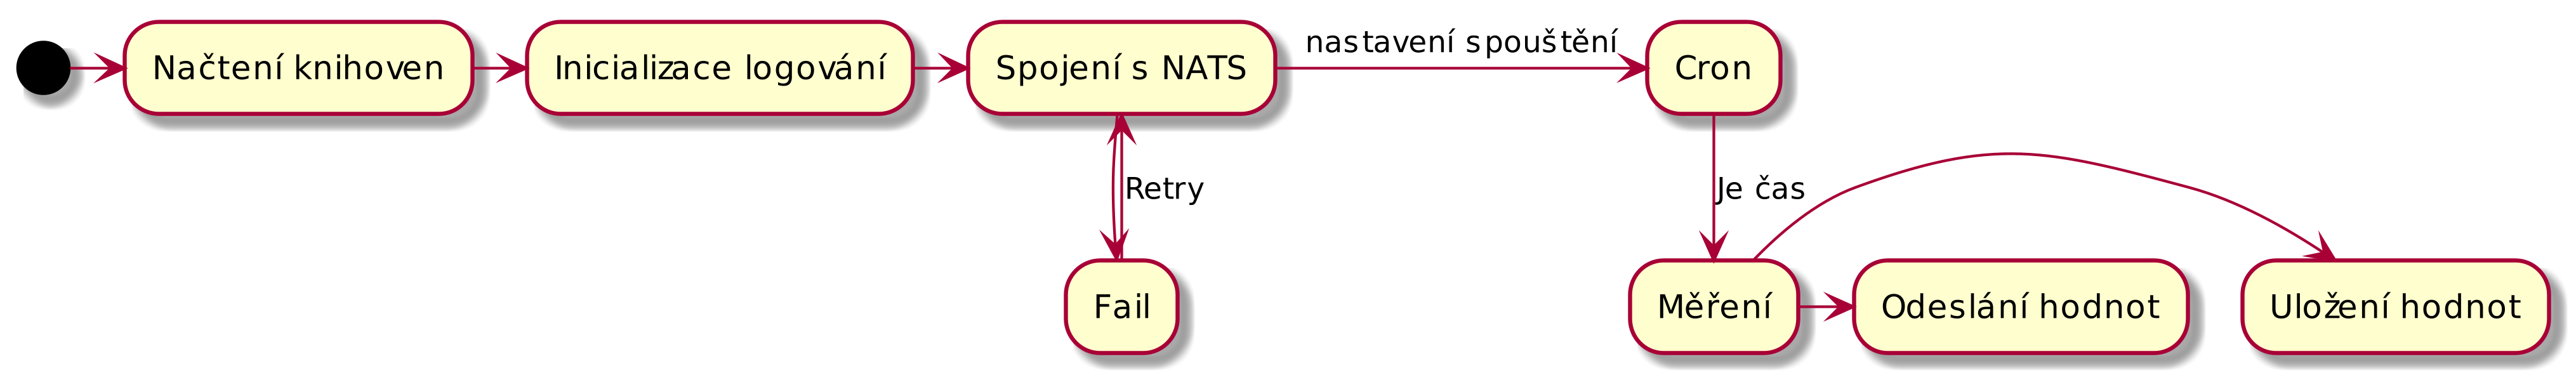
\includegraphics[width=\textwidth]{mereni.png}
    \caption{Průběh programu}
\end{figure}

Na začátku importuji šest \glslink{knihovna}{knihoven}, konkrétně používám části standardní \glslink{knihovna}{knihovny} 
pro práci s časem a operačním systémem, \glslink{knihovna}{knihovnu} pro práci s periferiemi a dále to jsou 
\glslink{knihovna}{knihovny} pro spojení s bránou, umožnění automatického spouštění programů v daný čas a logování. Ve 
funkci main, jako první nastavím \glslink{knihovna}{knihovnu} logrus, který mi zajišťuje logování, nastavuji co chci 
logovat, kam to má zapsat a jak to má zformátovat. Poté otevřu spojení s bránou, inicializuji 
\glslink{knihovna}{knihovnu} na použití periferií a nastavím cron, aby mi spustil měření každých 15 minut. Nakonec je 
takový trik, jehož jediným účelem je, aby hlavní gorutina neskončila, jedná se o čtení z kanálu do kterého, však nikdy 
nic nezapíši. A jelikož jde o blokující operaci, program nikdy neskončí.

% měření
\paragraph*{Měření}
Samotné získávání dat je velmi jednoduché. Každých 15 minut se zavolá funkce getMeasure(),která postupně projde přes 
všechny připojené senzory, zavolá funkce, které je obsluhují, v případě chyby je zkouší zavolat vícekrát a vrátí pole 
s naměřenými hodnotami. Pro měření jsem se snažil co nejvíce využít možností, které poskytuje  \gls{knihovna} 
\gls{periphio}, takže například data vracím ve formě struktury z této knihovny a používám ji pro získávání hodnot ze 
dvou senzorů, pro třetí ji nepoužívám jen z toho důvodu, že ho zatím nepodporuje. Měření z BME280 je velmi jednoduché. 
V podstatě otevřu sběrnici, přečtu data a vrátím je, vše za použití výše zmíněné knihovny. Z DS18B20 to je velmi podobné, 
jen nemohu použít \gls{periphio}, takže používám knihovnu, jež využívá modul kernelu, který zpřístupňuje tento senzor 
přes virtuální souborový systém. Senzor DHT11 je na použití asi nejsložitější. Používám sice externí knihovnu, avšak ta 
pro přístup ke GPIO využívá \gls{periphio}. Jinak je měření velmi obdobné jako u ostatních čidel, s tím rozdílem, že je 
velmi chybové, takže se musí vícekrát opakovat.

\paragraph*{DHT11}
S tímto senzorem jsem měl asi největší problémy. Nejenom že jsem musel laborovat s nastavením verze api knihovny 
periph.io, ale i samotná knihovna pro obsluhu senzoru obsahovala chyby. Takže jsem ji důkladně prozkoumal a porovnal 
s datasheetem(\url{https://www.mouser.com/datasheet/2/758/DHT11-Technical-Data-Sheet-Translated-Version-1143054.pdf}) 
k senzoru. Našel jsem dvě zásadní chyby. Jedna byla, že knihovna vyslal příliš krátký startovací pulz, takže ani čidlo 
neprobudila, to se dalo vyřešit jednoduše, prostě jsem do programu přidal pauzu. A druhá, že špatně zpracovávala data co 
z čidla četla. Před úpravou mi vracela nereálné hodnoty teploty a vlhkosti, konkrétně vracela chybu, že načtená data 
jsou mimo rozsah, protože hodnoty zpracovávala jako jedno velké šestnáctibitové číslo, ale v datasheetu jsem se dočetl 
že tyto dva bajty představují číslo v desetinné čárce, ale velmi neobvykle. První bajt je celá část a druhý desetinná 
a zároveň s tím se v datasheetu píše že rozlišovací schopnost senzoru je 1 \textdegree C a 1 \%, takže jsem druhý bajt 
zahodil a dál pracoval pouze s tím prvním. A to fungovalo na jedničku. Tuto zvláštnost s rozlišením bych asi vysvětlil 
tím, že komunikační protokol bude schodný i s dražšími senzory s lepším rozlišením a to možná souvisí i s chybami 
v knihovně, poněvadž je určena i pro ně. Takže abych jejich podporu nerozbil jsem mé úpravy podmínil použitím správného 
typu čidla. Moje upravená verze kterou používám, je k nalezení zde: \url{https://github.com/prokopparuzek/go-dht.git}.

% ukládání dat
\paragraph*{Ukládání}
Pro ukládání dat na měřící stanici jsem nevymýšlel nic složitého. Vezmu jen data z každého senzoru, přidám 
\gls{timestamp}, tím se vyhnu problémům s reprezentací času a převody časových pásem a to vše přidám za konec souboru 
konkrétního senzoru. Data ukládám ve formátu \acrshort{csv}. Jednotlivé hodnoty/sloupce nijak neoznačuji, nechávám to na 
utilitách, jejichž cílem bude data obnovit, ty jediné s nimi takto budou pracovat a to jen občas, takže to myslím 
nevadí, a navíc to zjednodušuje kód.

\paragraph*{Message broker}
Jako základní \gls{message-broker} by se dal použít server NATS. Já použiji trochu bezpečnější variantu, konkrétně 
použiji nadstavbu nazývanou NATS-streaming. Stejně jako NATS se jedná o lehkou aplikaci napsanou v go, takže zabírá 
minimum zdrojů \parencite{root.cz:NATS-streaming}. Já jsem ji vybral z důvodu jednoduchosti, dostupnosti široké škály 
klientských knihoven a též již zmiňované lehkosti. A taky proto že mám rád go.

% odesílání
\paragraph*{Odesílání}
Odesílání dat začíná vlastně už na úplném začátku, kdy se spojím se serverem a pak až do konce držím spojení otevřené. 
Samotné odeslání dat do \glslink{message-broker}{message brokera}, se vlastně moc neliší od uložení. Taky vezmu data, 
přidám \gls{timestamp} a pošlu je. Je tu však pár rozdílů. Data posílám ve formátu \gls{JSON}, který je jednoduchý 
a čitelný. Z důvodu možných latencí, nedostupnosti sítě\ldots odesílám každou zprávu v samostatné 
\glslink{gorutina}{gorutině}, abych neblokoval další měření, jelikož když se zprávu nepovede odeslat, tak ji zkouším 
poslat po minutě další zhruba dvě hodiny. No a to je vše po odeslání zprávy už nemusím nic řešit, poněvadž server si ji 
uloží a pošle dál, takže už se neztratí.

\section{Cloud}
% výběr
Na internetu se dá najít spoustu cloudových řešení, které bych mohl využít. Já jsem zvolil platformu \gls{firebase} od 
Googlu. Upřednostnil jsem ji před jinými řešeními, z nichž některá byla přímo vytvořená pro sběr a zobrazení dat 
z chytrých senzorů. Důvodů bylo několik. Řešení vytvořená \uv{na míru} měla zásadní problém v tom, že většinou v tarifu 
zdarma měla nějaké významné omezení, například omezení ukládaných dat pouze na poslední tři měsíce a platit se mi 
nechtělo(\url{https://io.adafruit.com/}). Z ostatních jsem vybral právě \gls{firebase}, poněvadž měl rozumně nastavené 
limity zdarma, nádhernou dokumentaci a zároveň za ním stojí velká firma, takže se nemusím bát, že za rok 
skončí(\url{https://firebase.google.com/pricing}).

\subsection{Firebase}
% založení
\gls{firebase} je služba Googlu, takže jediné co je potřeba pro založení je Google účet, díky tarifu zdarma ani nechce 
žádnou platební kartu. Založení projektu se pokusím osvětlit několika obrázky. Počáteční adresa je 
\url{https://console.firebase.google.com/u/0/}

% krok 1
\begin{figure}[H]
    \centering
    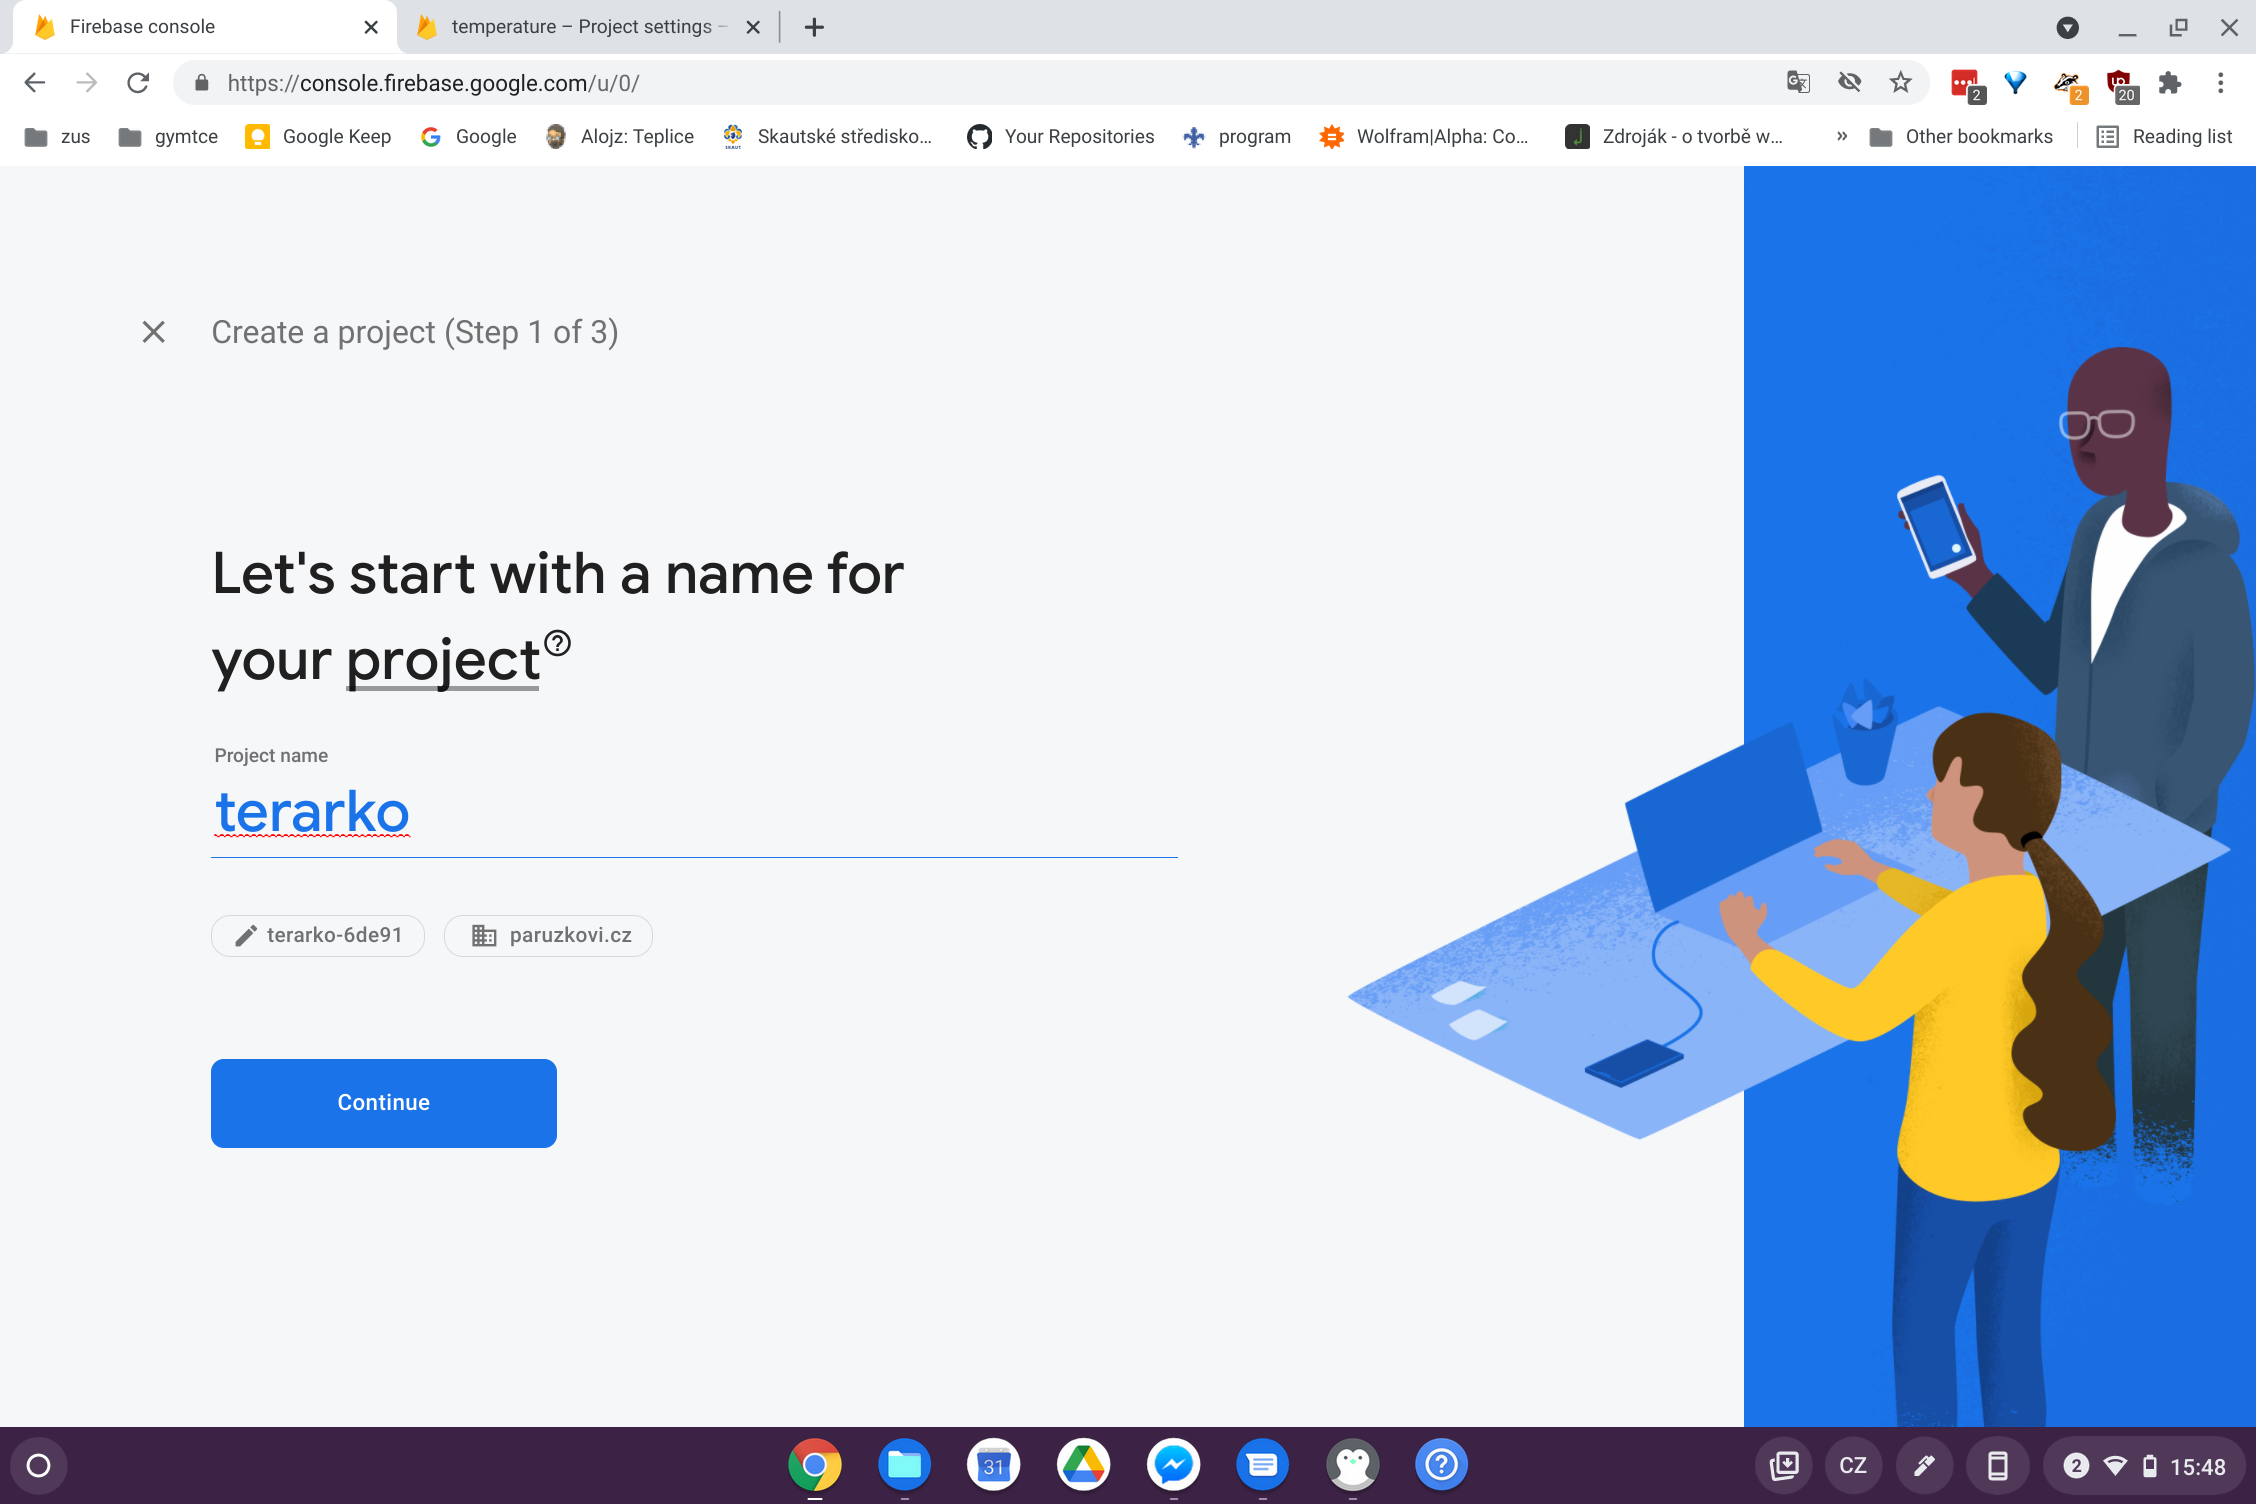
\includegraphics[width=0.8\textwidth]{firebase-1.png}
    \caption{Firebase, krok 1}
\end{figure}
V kroku 1 vybírám projektu jméno.
%krok 2
\begin{figure}[H]
    \centering
    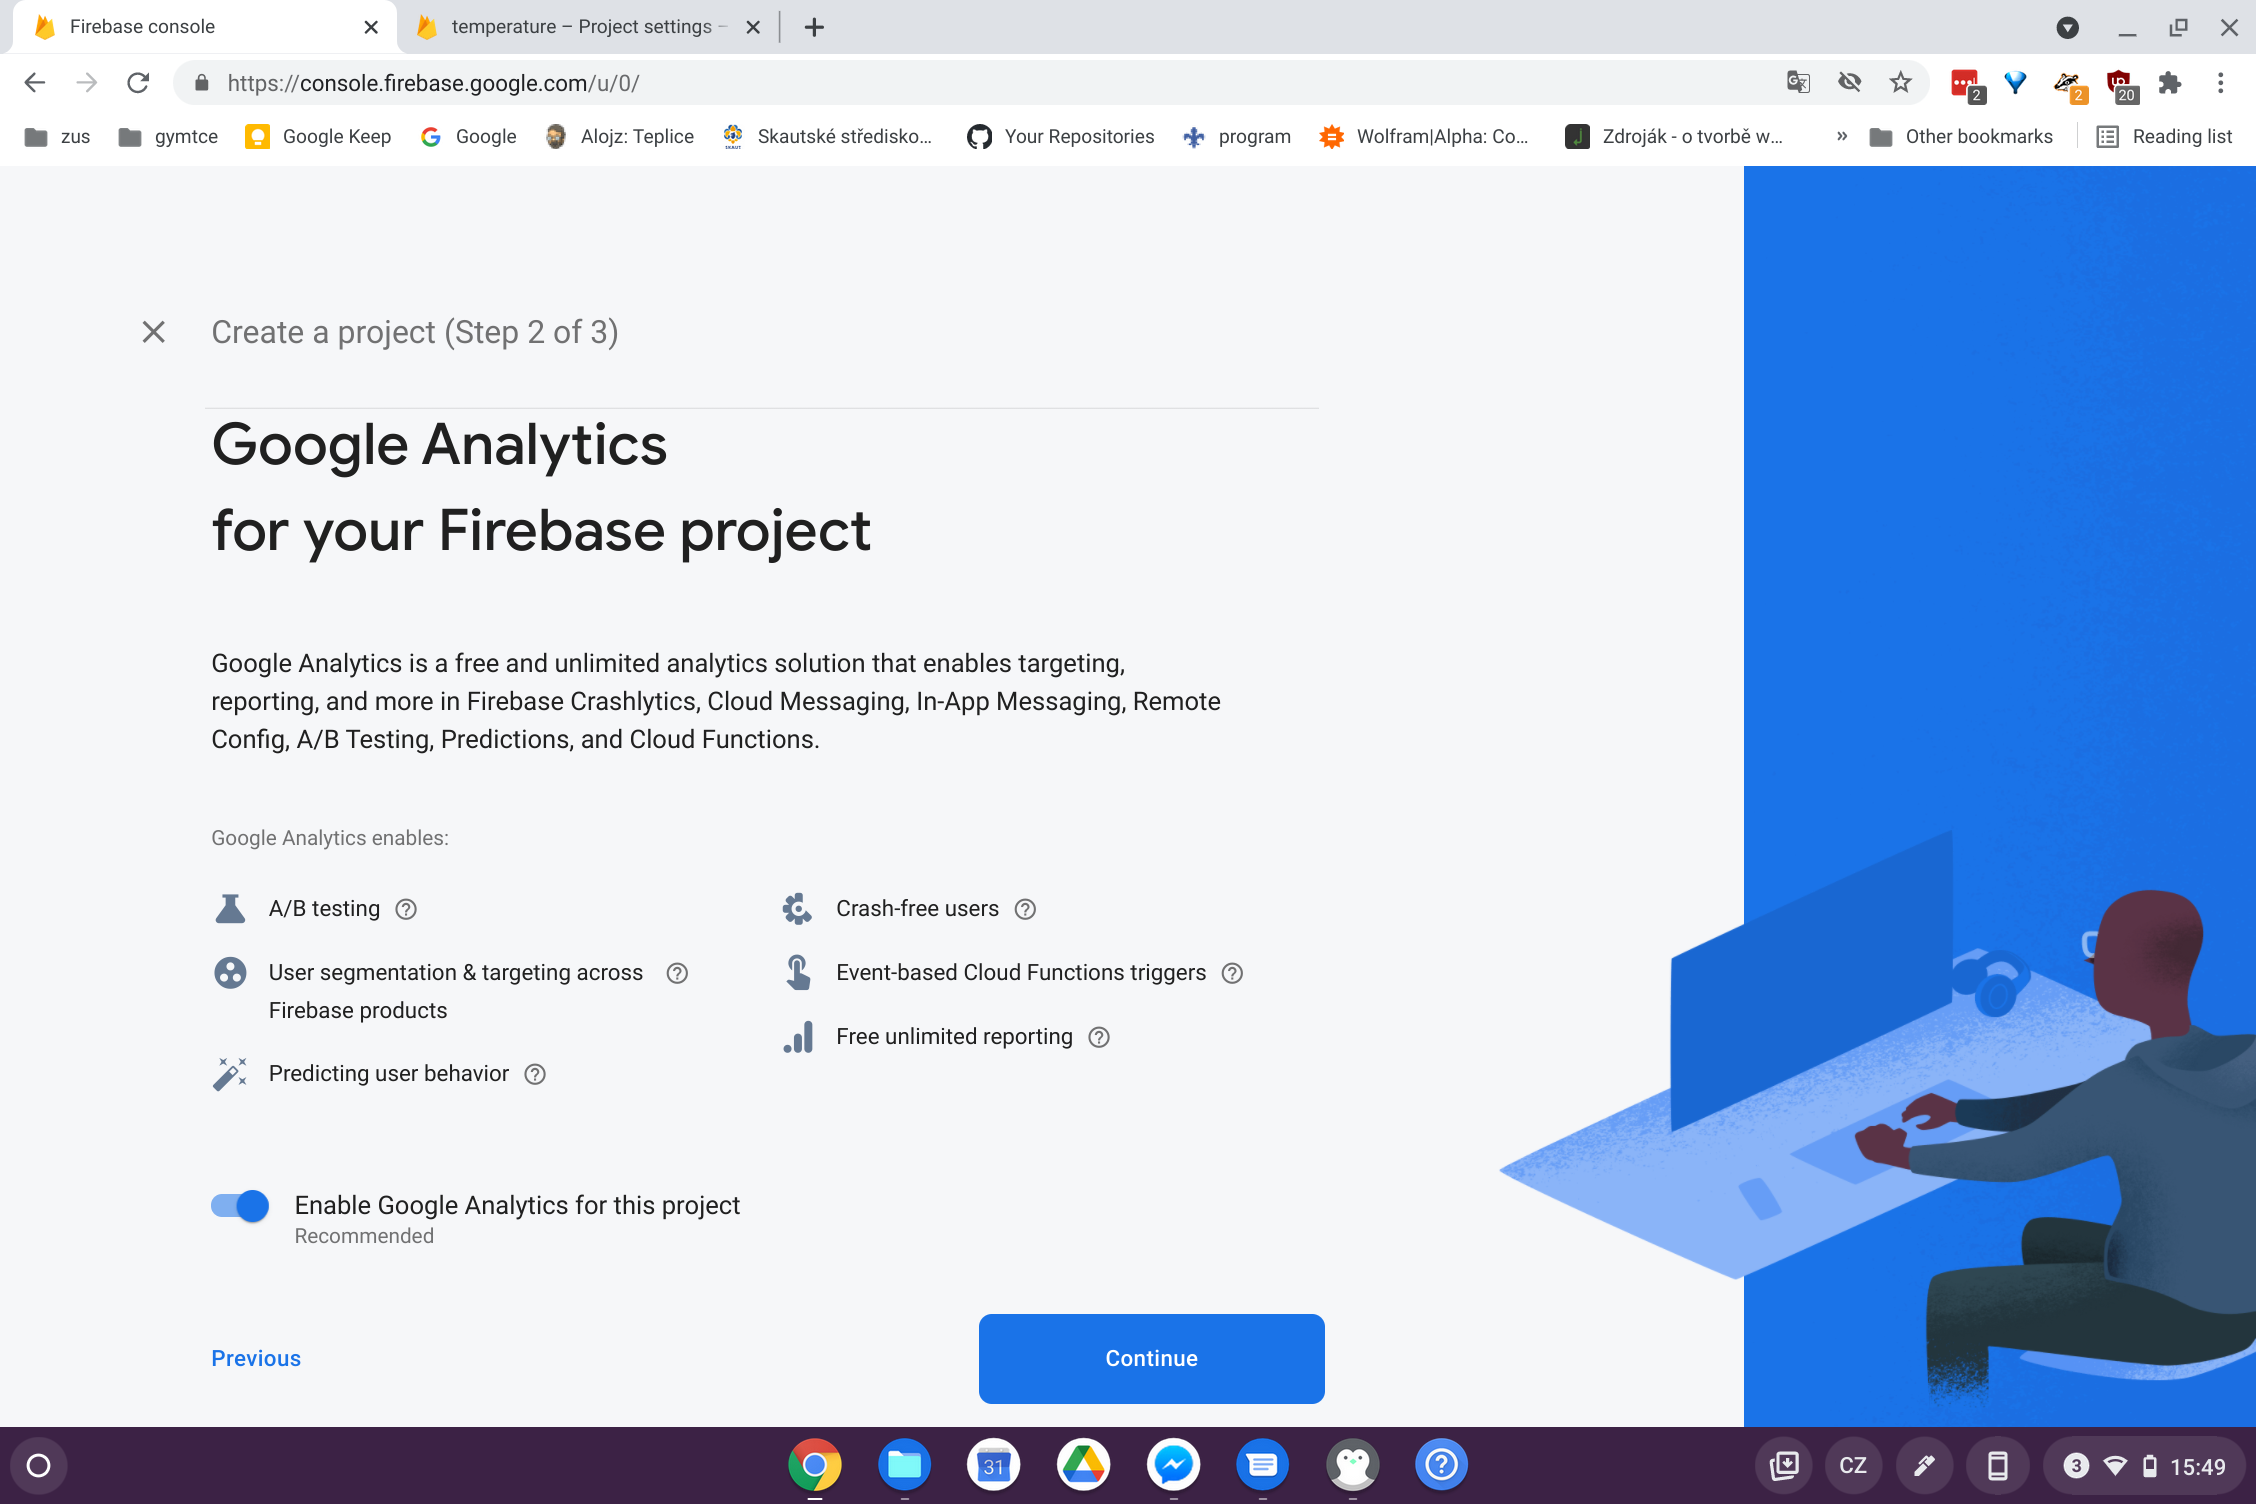
\includegraphics[width=0.8\textwidth]{firebase-2.png}
    \caption{Firebase, krok 2}
\end{figure}
V kroku 2 můžu pro projekt povolit Google Analytics.
% krok 3
\begin{figure}[H]
    \centering
    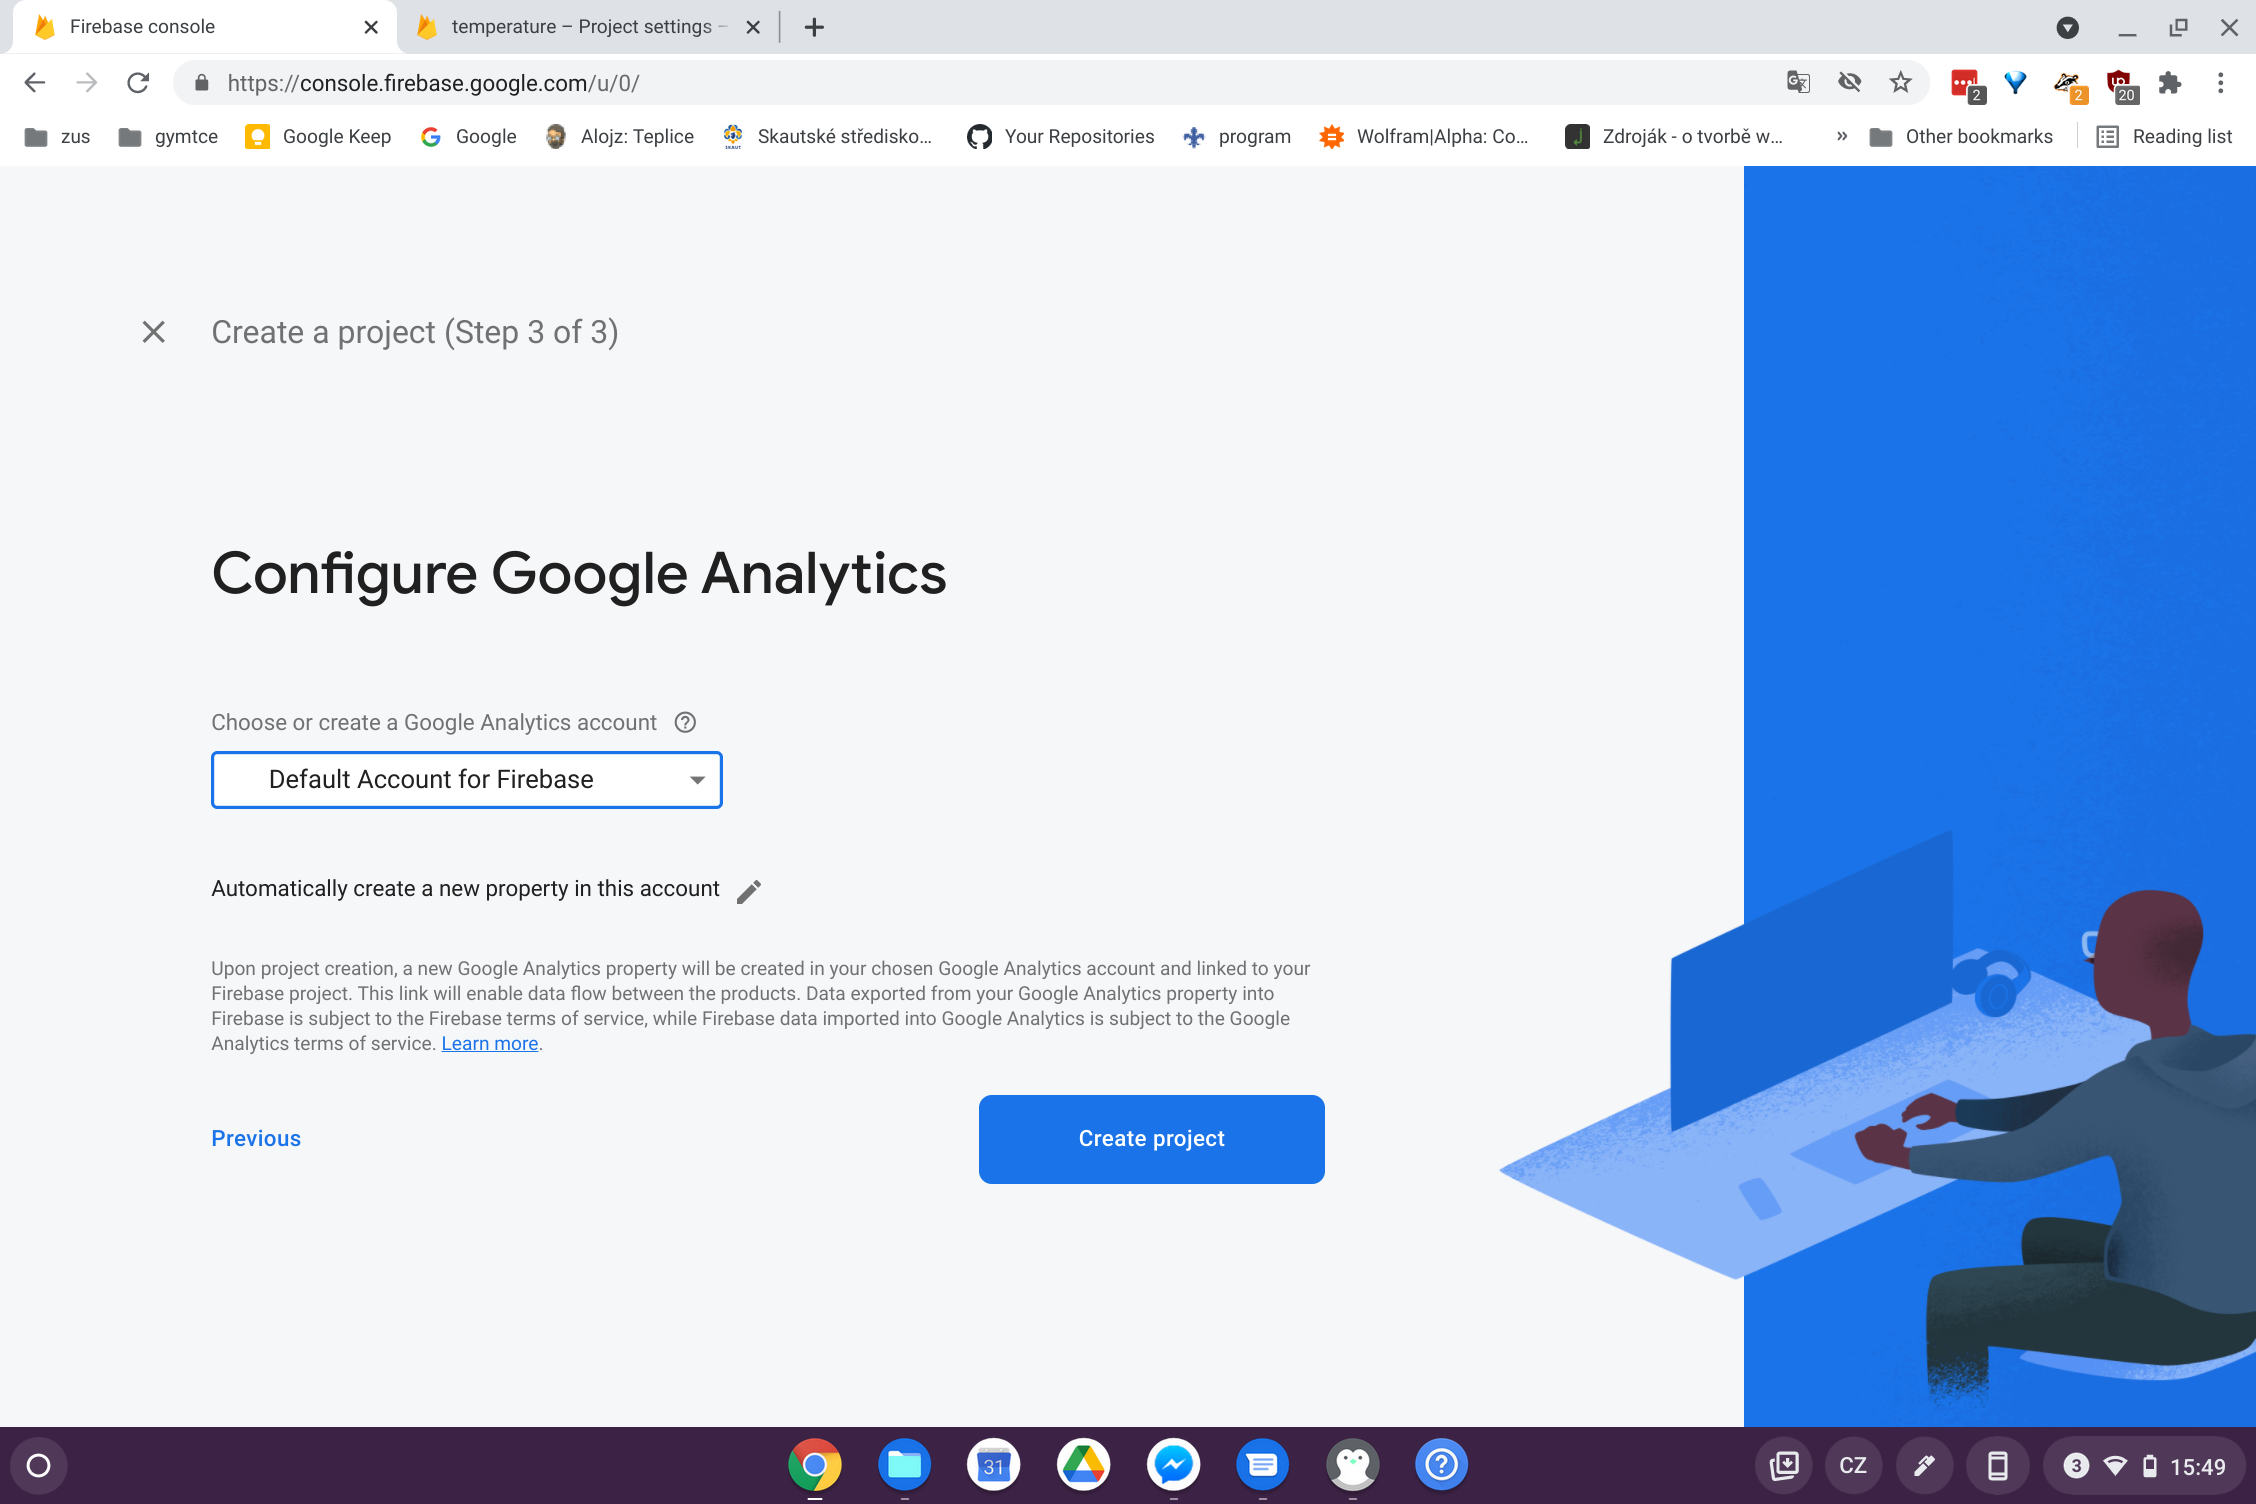
\includegraphics[width=0.8\textwidth]{firebase-3.png}
    \caption{Firebase, krok 3}
\end{figure}
V kroku 3 přiřazuji účet Google Analytics.% hotovo
\begin{figure}[H]
    \centering
    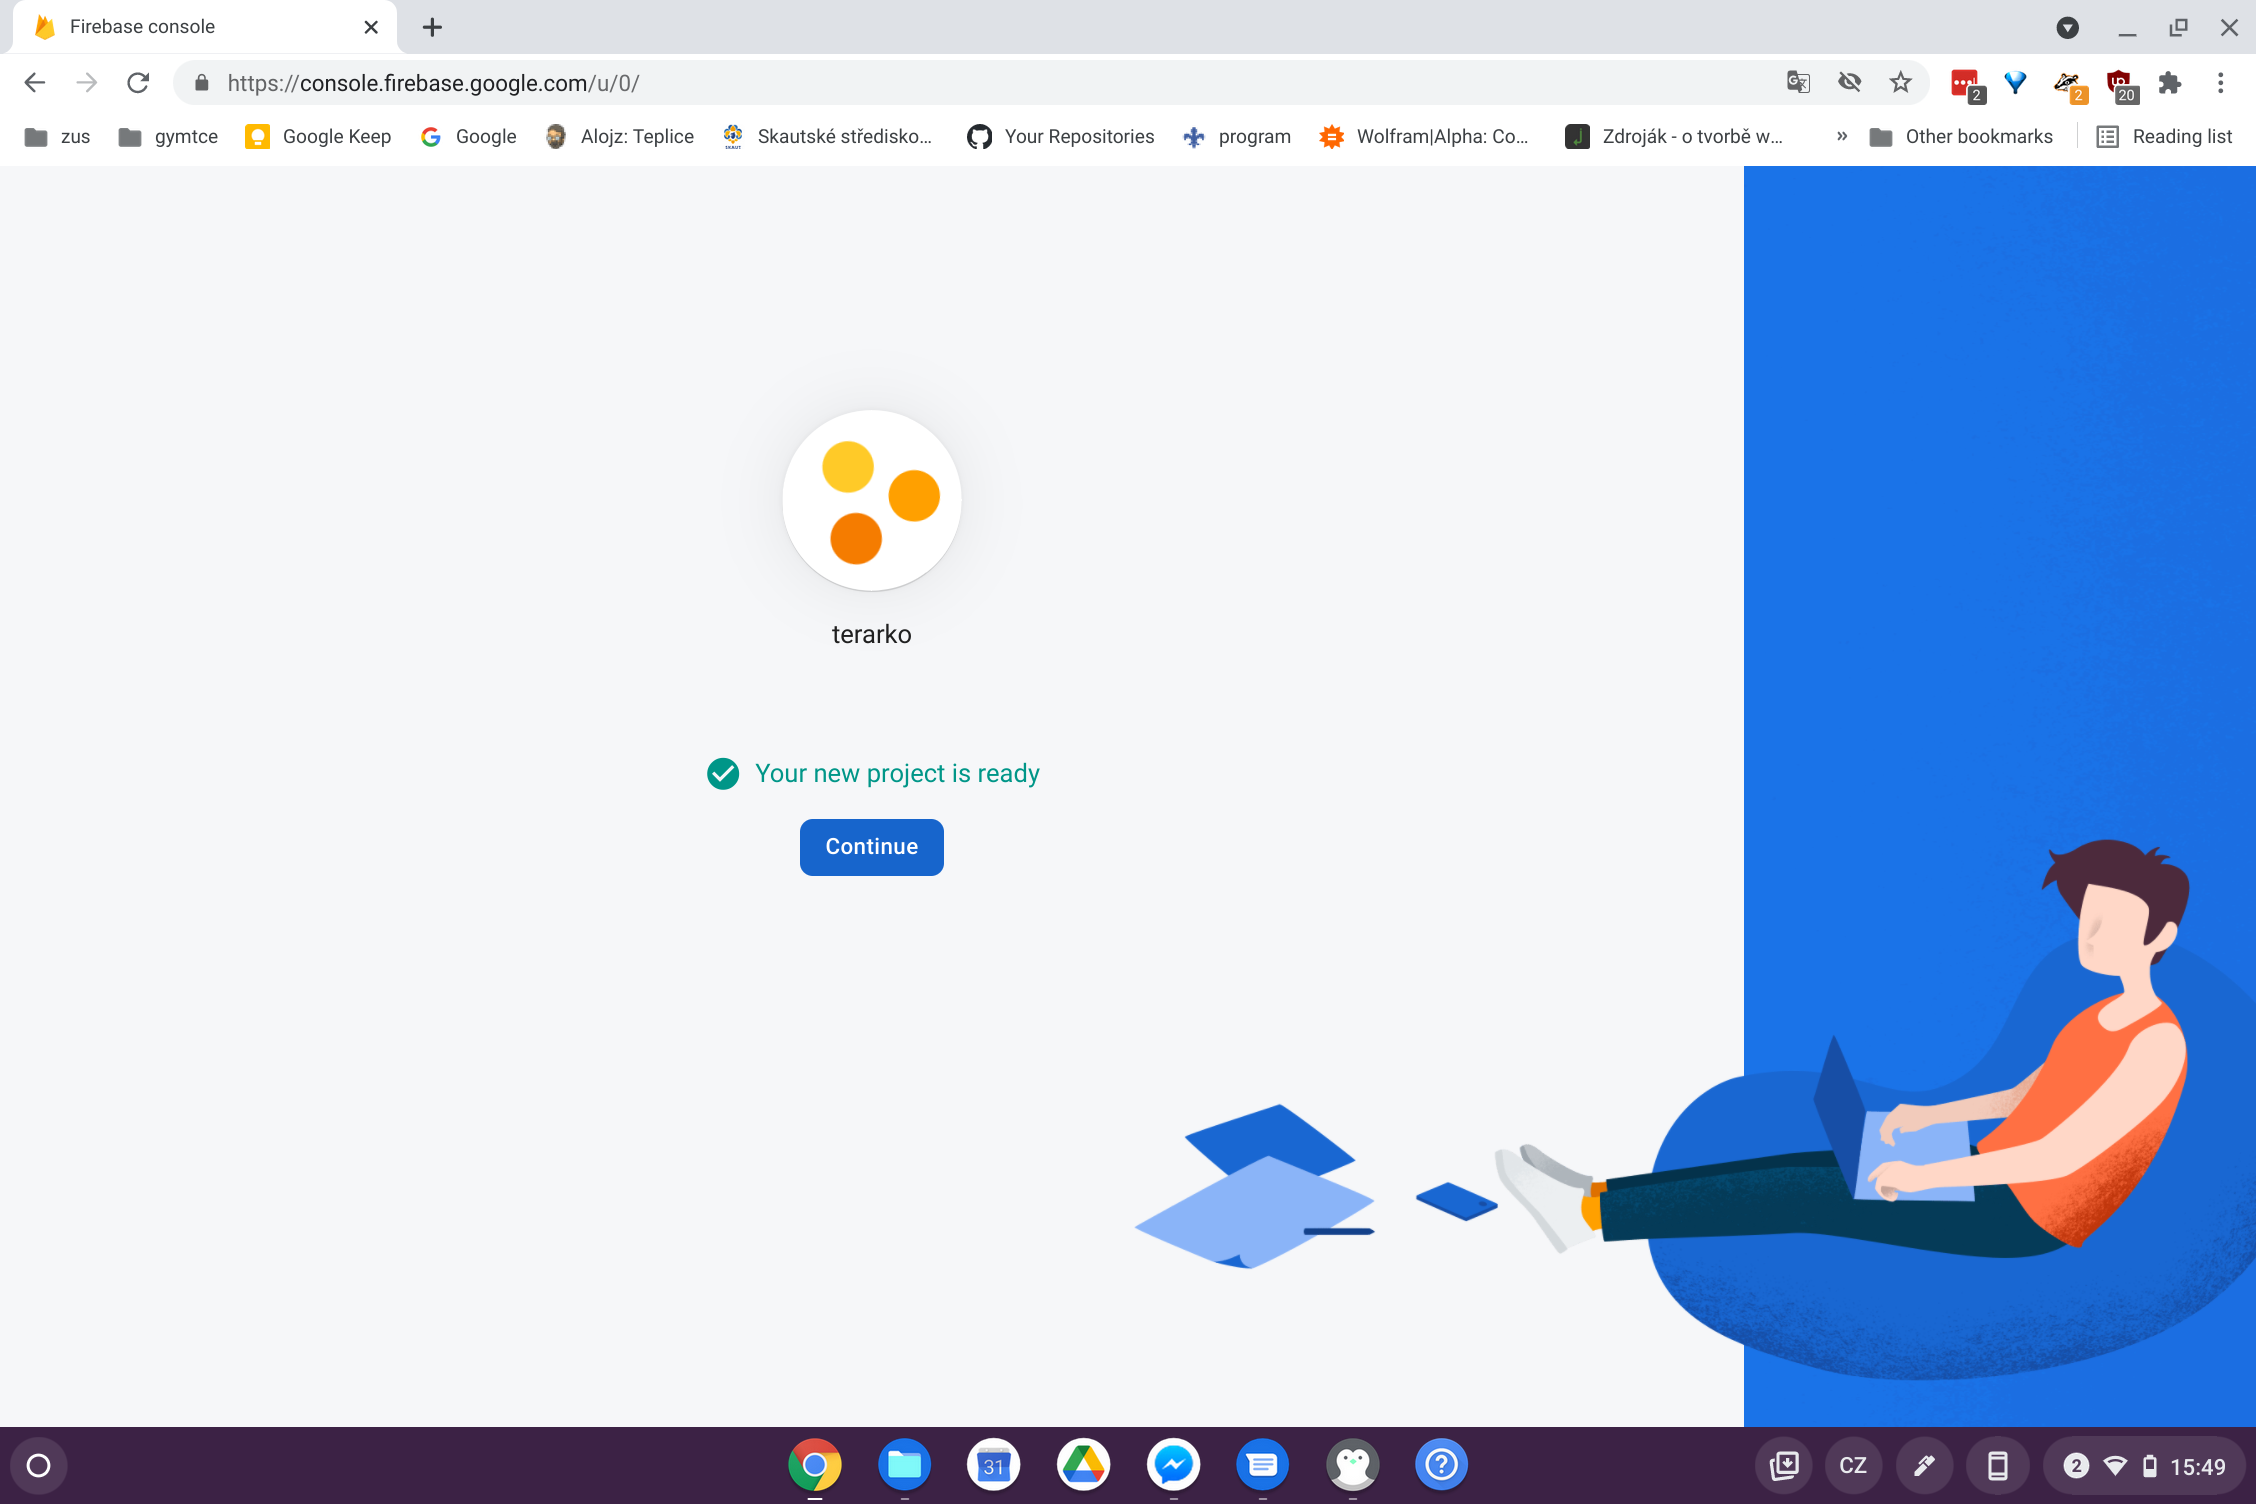
\includegraphics[width=0.8\textwidth]{firebase-fin.png}
    \caption{Firebase, hotovo}
\end{figure}
Vše jsem ponechal na výchozích hodnotách, teoreticky bych vzhledem k účelu mohl vypnout Google Analytics.
% dashboard
\begin{figure}[H]
    \centering
    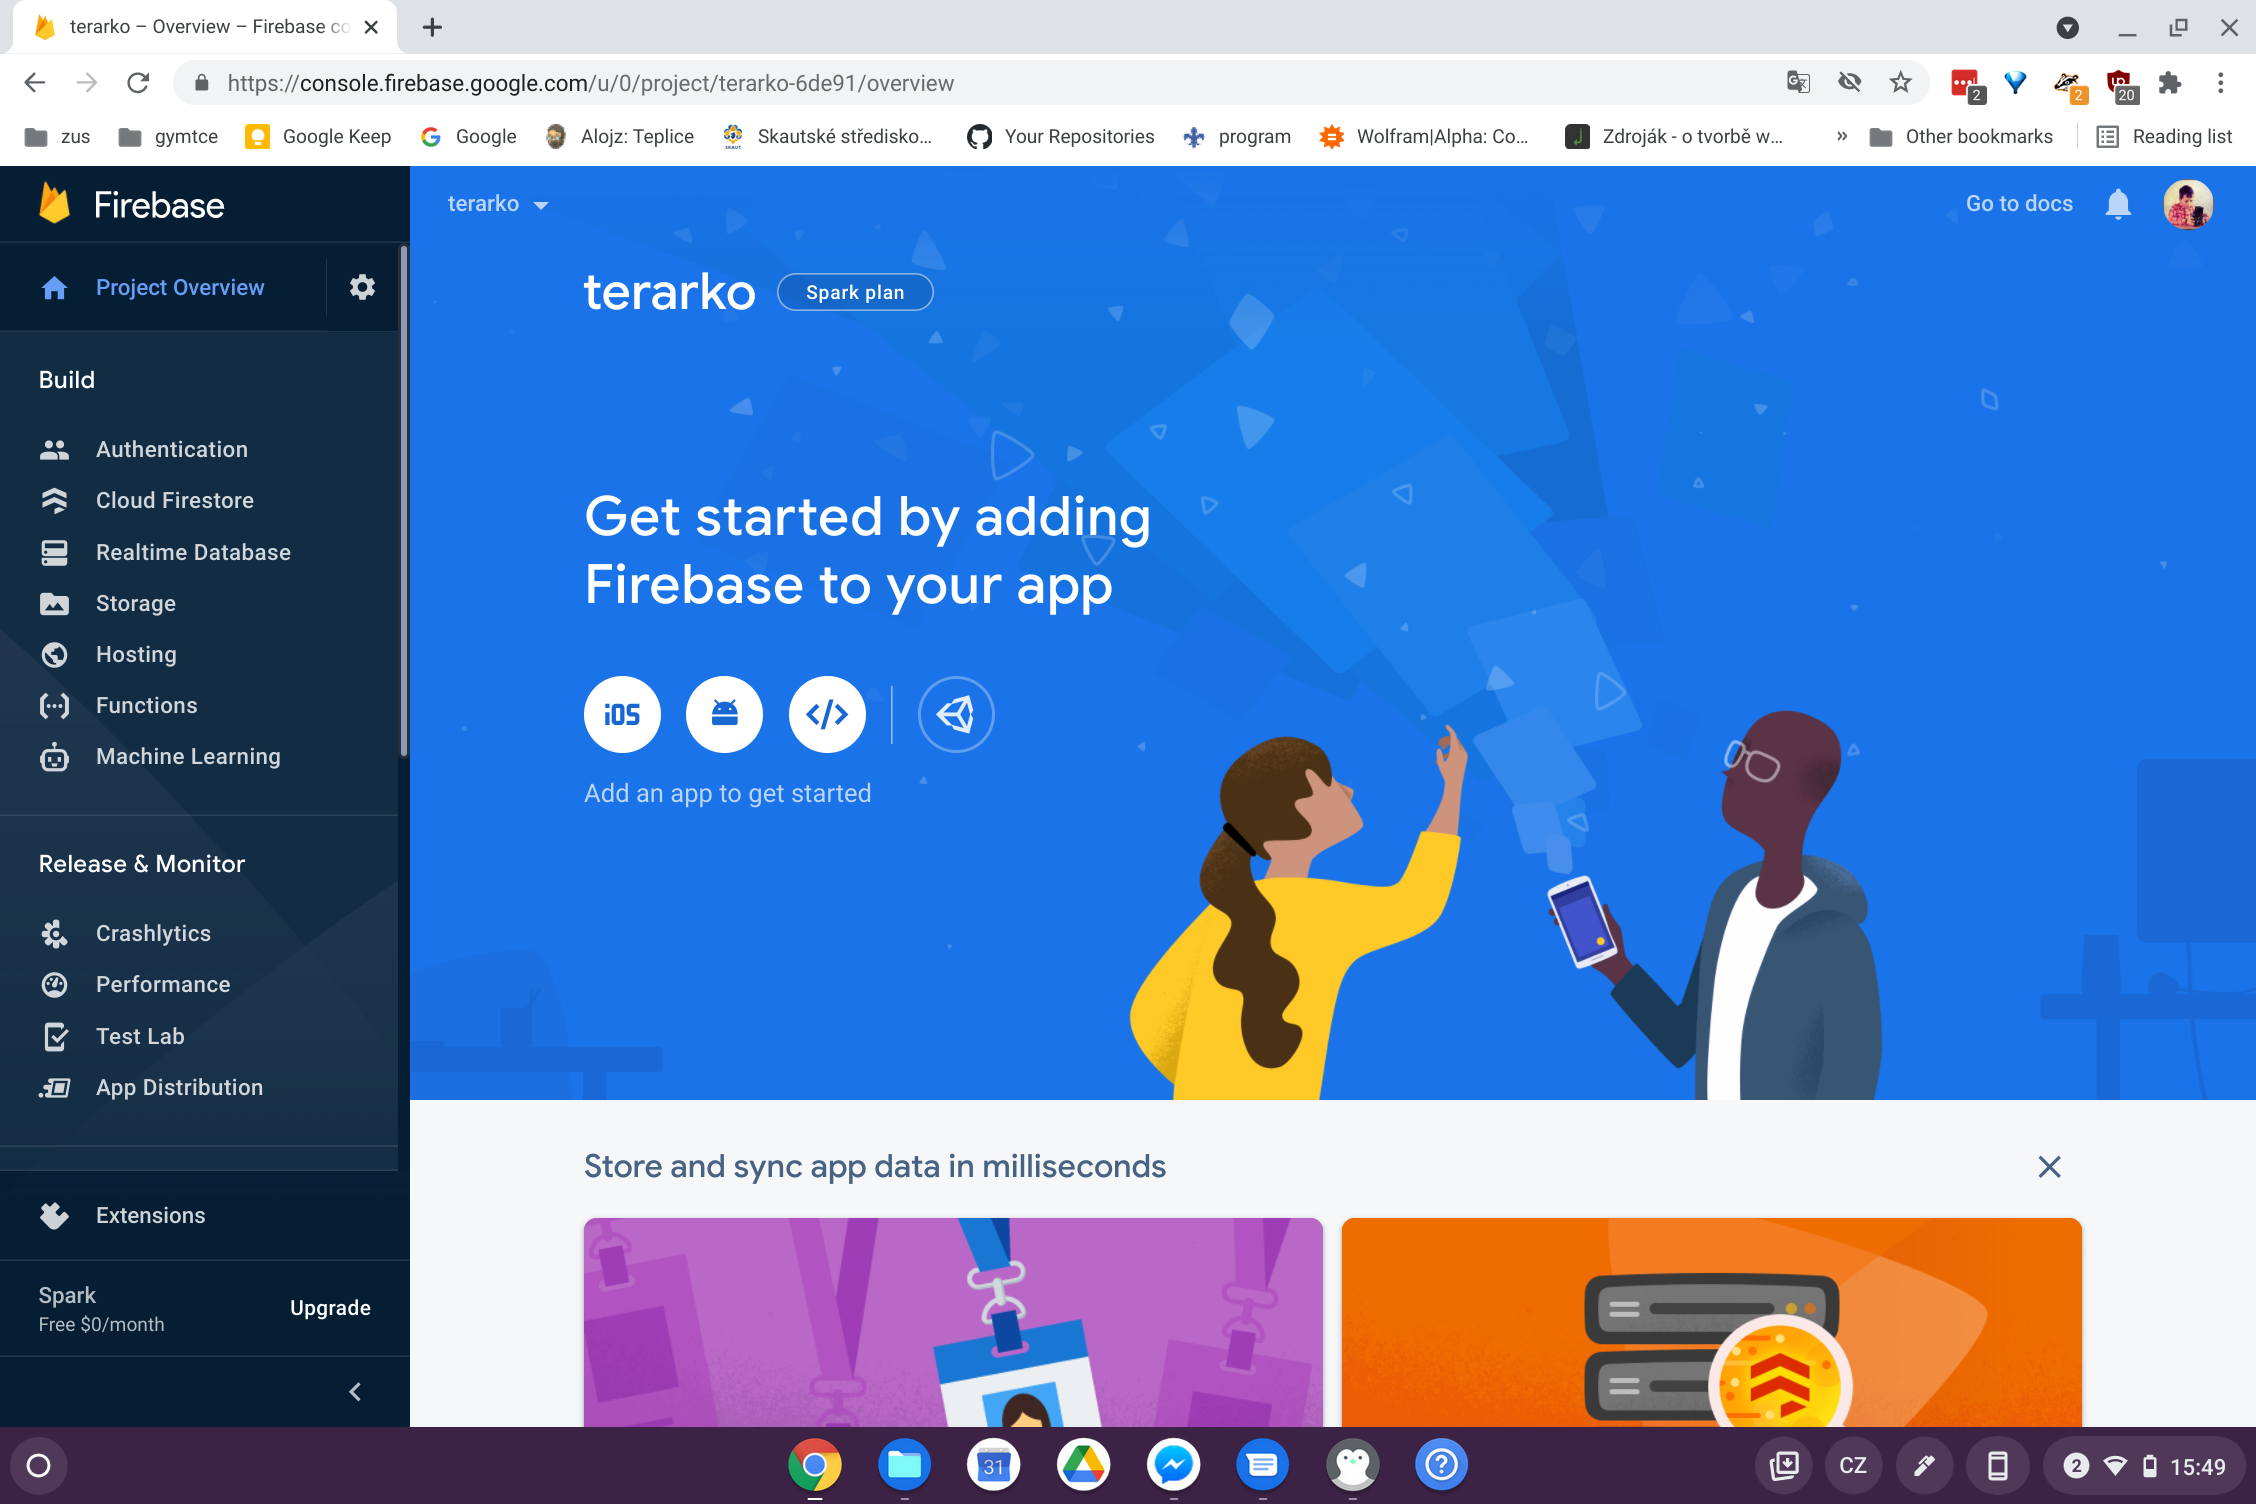
\includegraphics[width=0.8\textwidth]{firebase-dashboard.png}
    \caption{Firebase}
\end{figure}
Takto vypadá úvodní stránka \gls{firebase} po založení. Teď můžu přidat aplikace, které budu používat.

\subsection{Firestore}
Jako první přidám firestore, což je rychlá \gls{nosql} databáze, kterou budu používat pro ukládání naměřených hodnot. 
Opět se pokusím vysvětlit několika obrázky.

% krok 1
\begin{figure}[H]
    \centering
    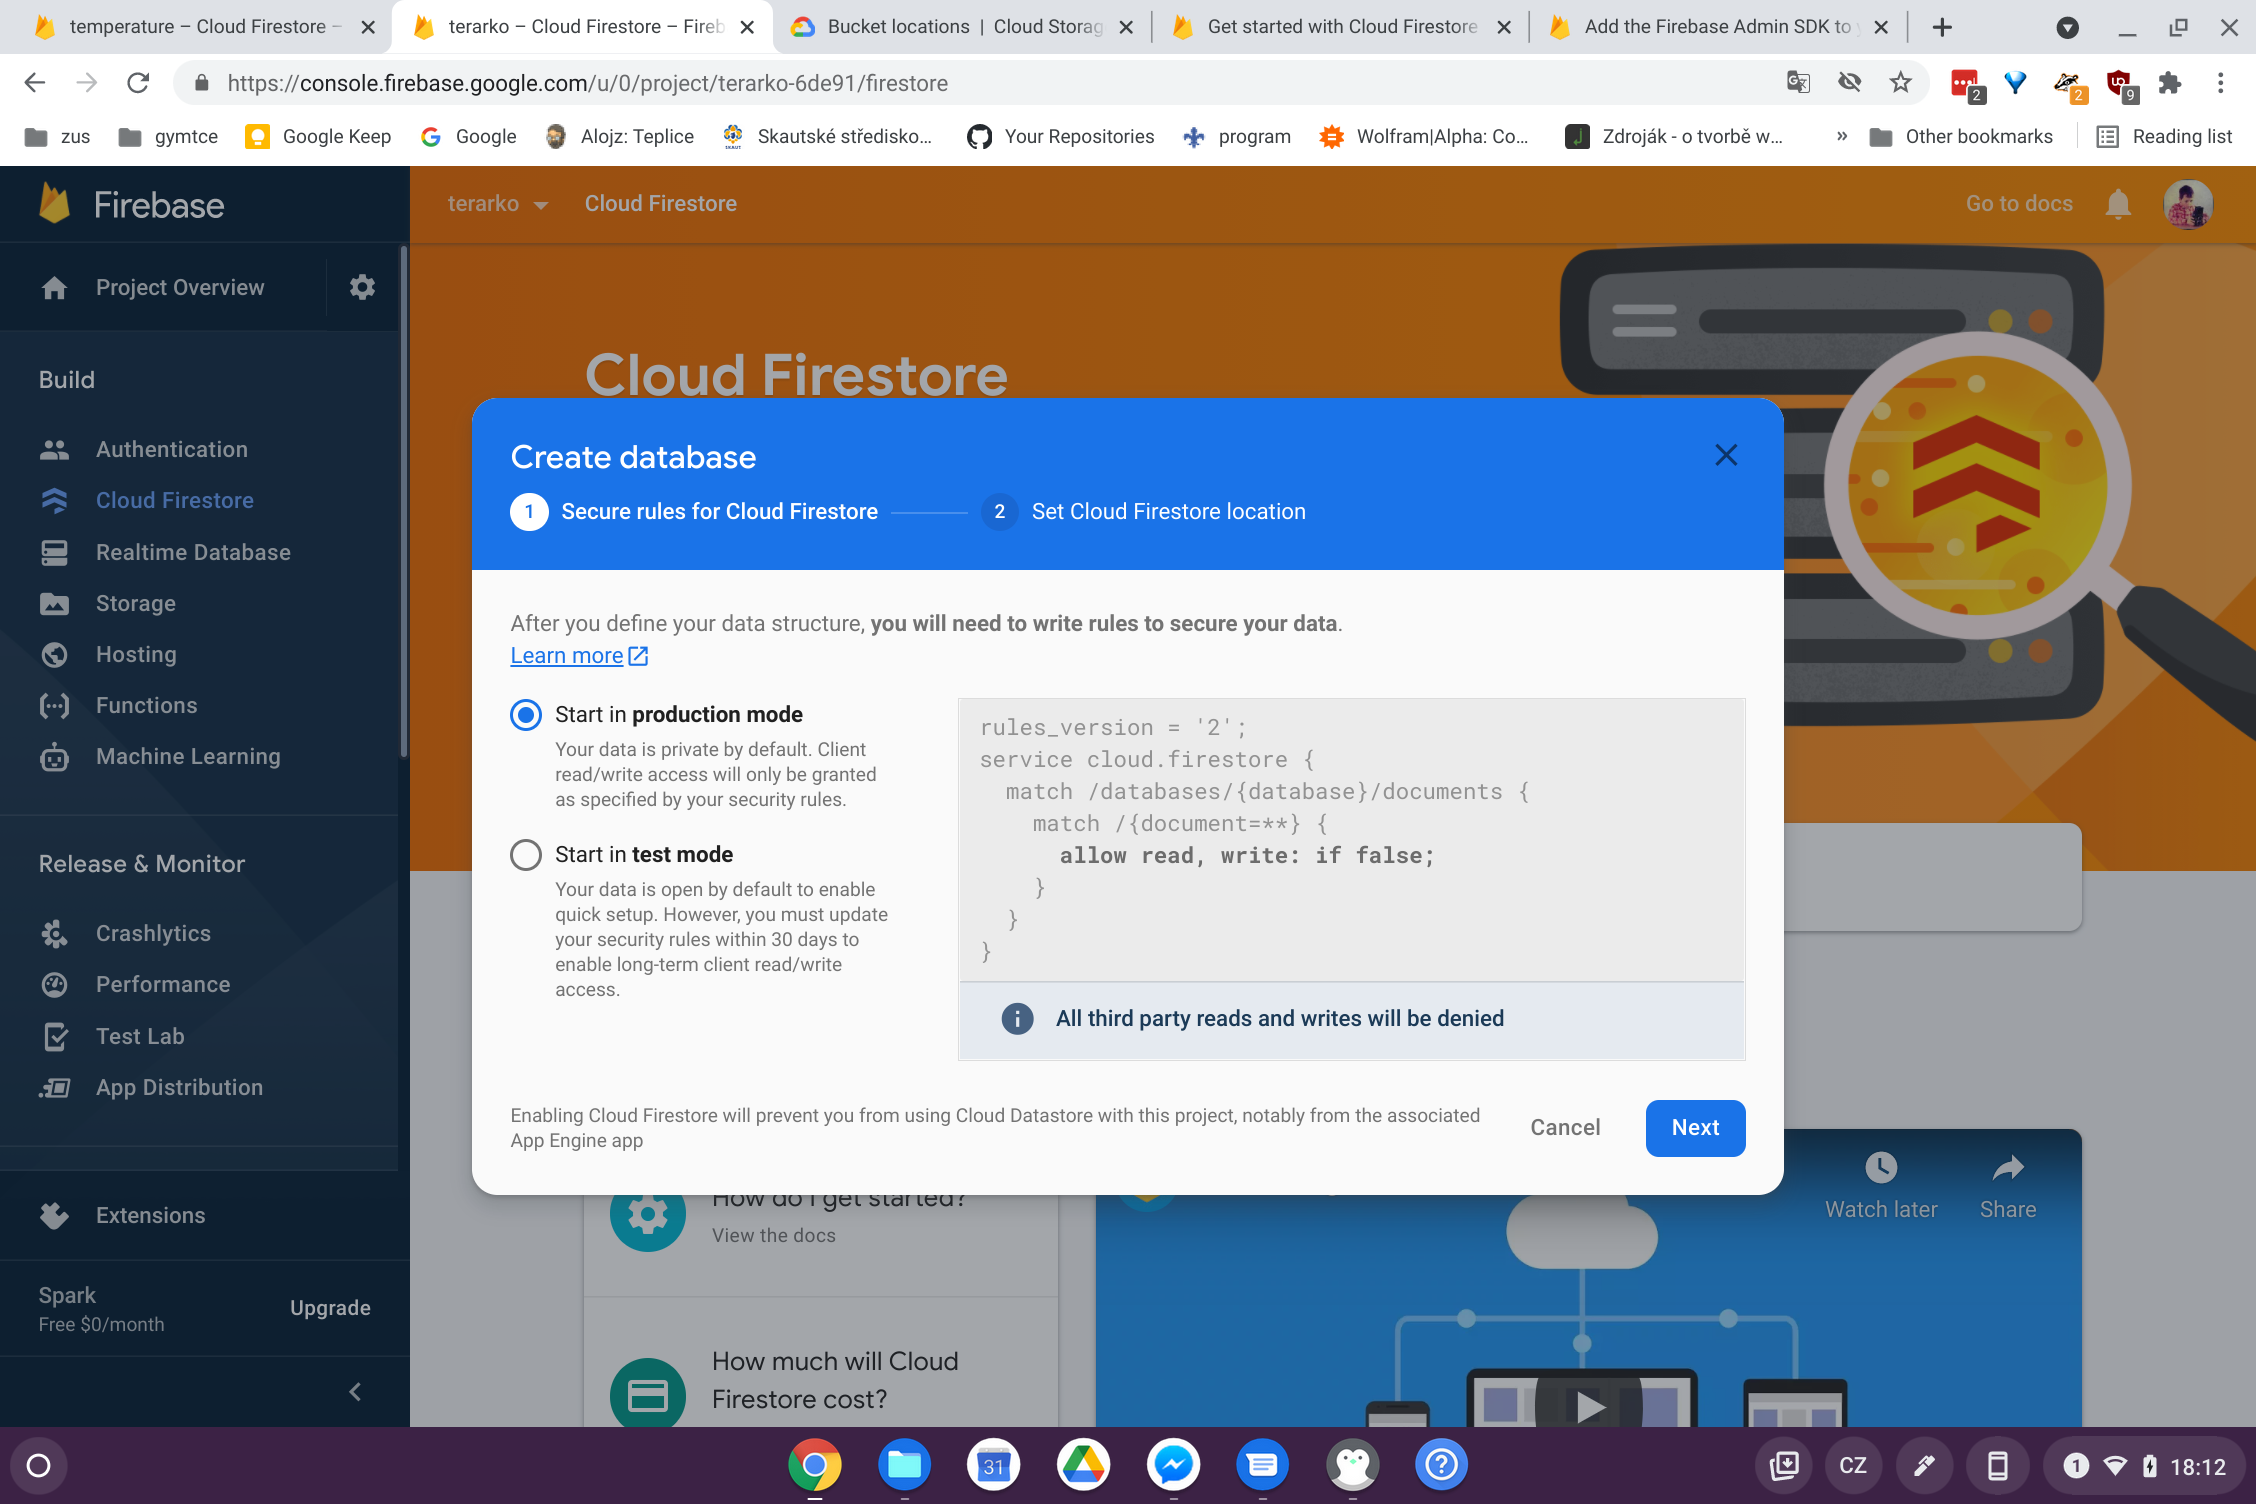
\includegraphics[width=0.8\textwidth]{firestore-1.png}
    \caption{Firestore, krok 1}
\end{figure}
Nastavení bezpečnosti použiji v produkčním módu, nechci aby se mi tam někdo připojoval bez přihlášení.
% krok 2
\begin{figure}[H]
    \centering
    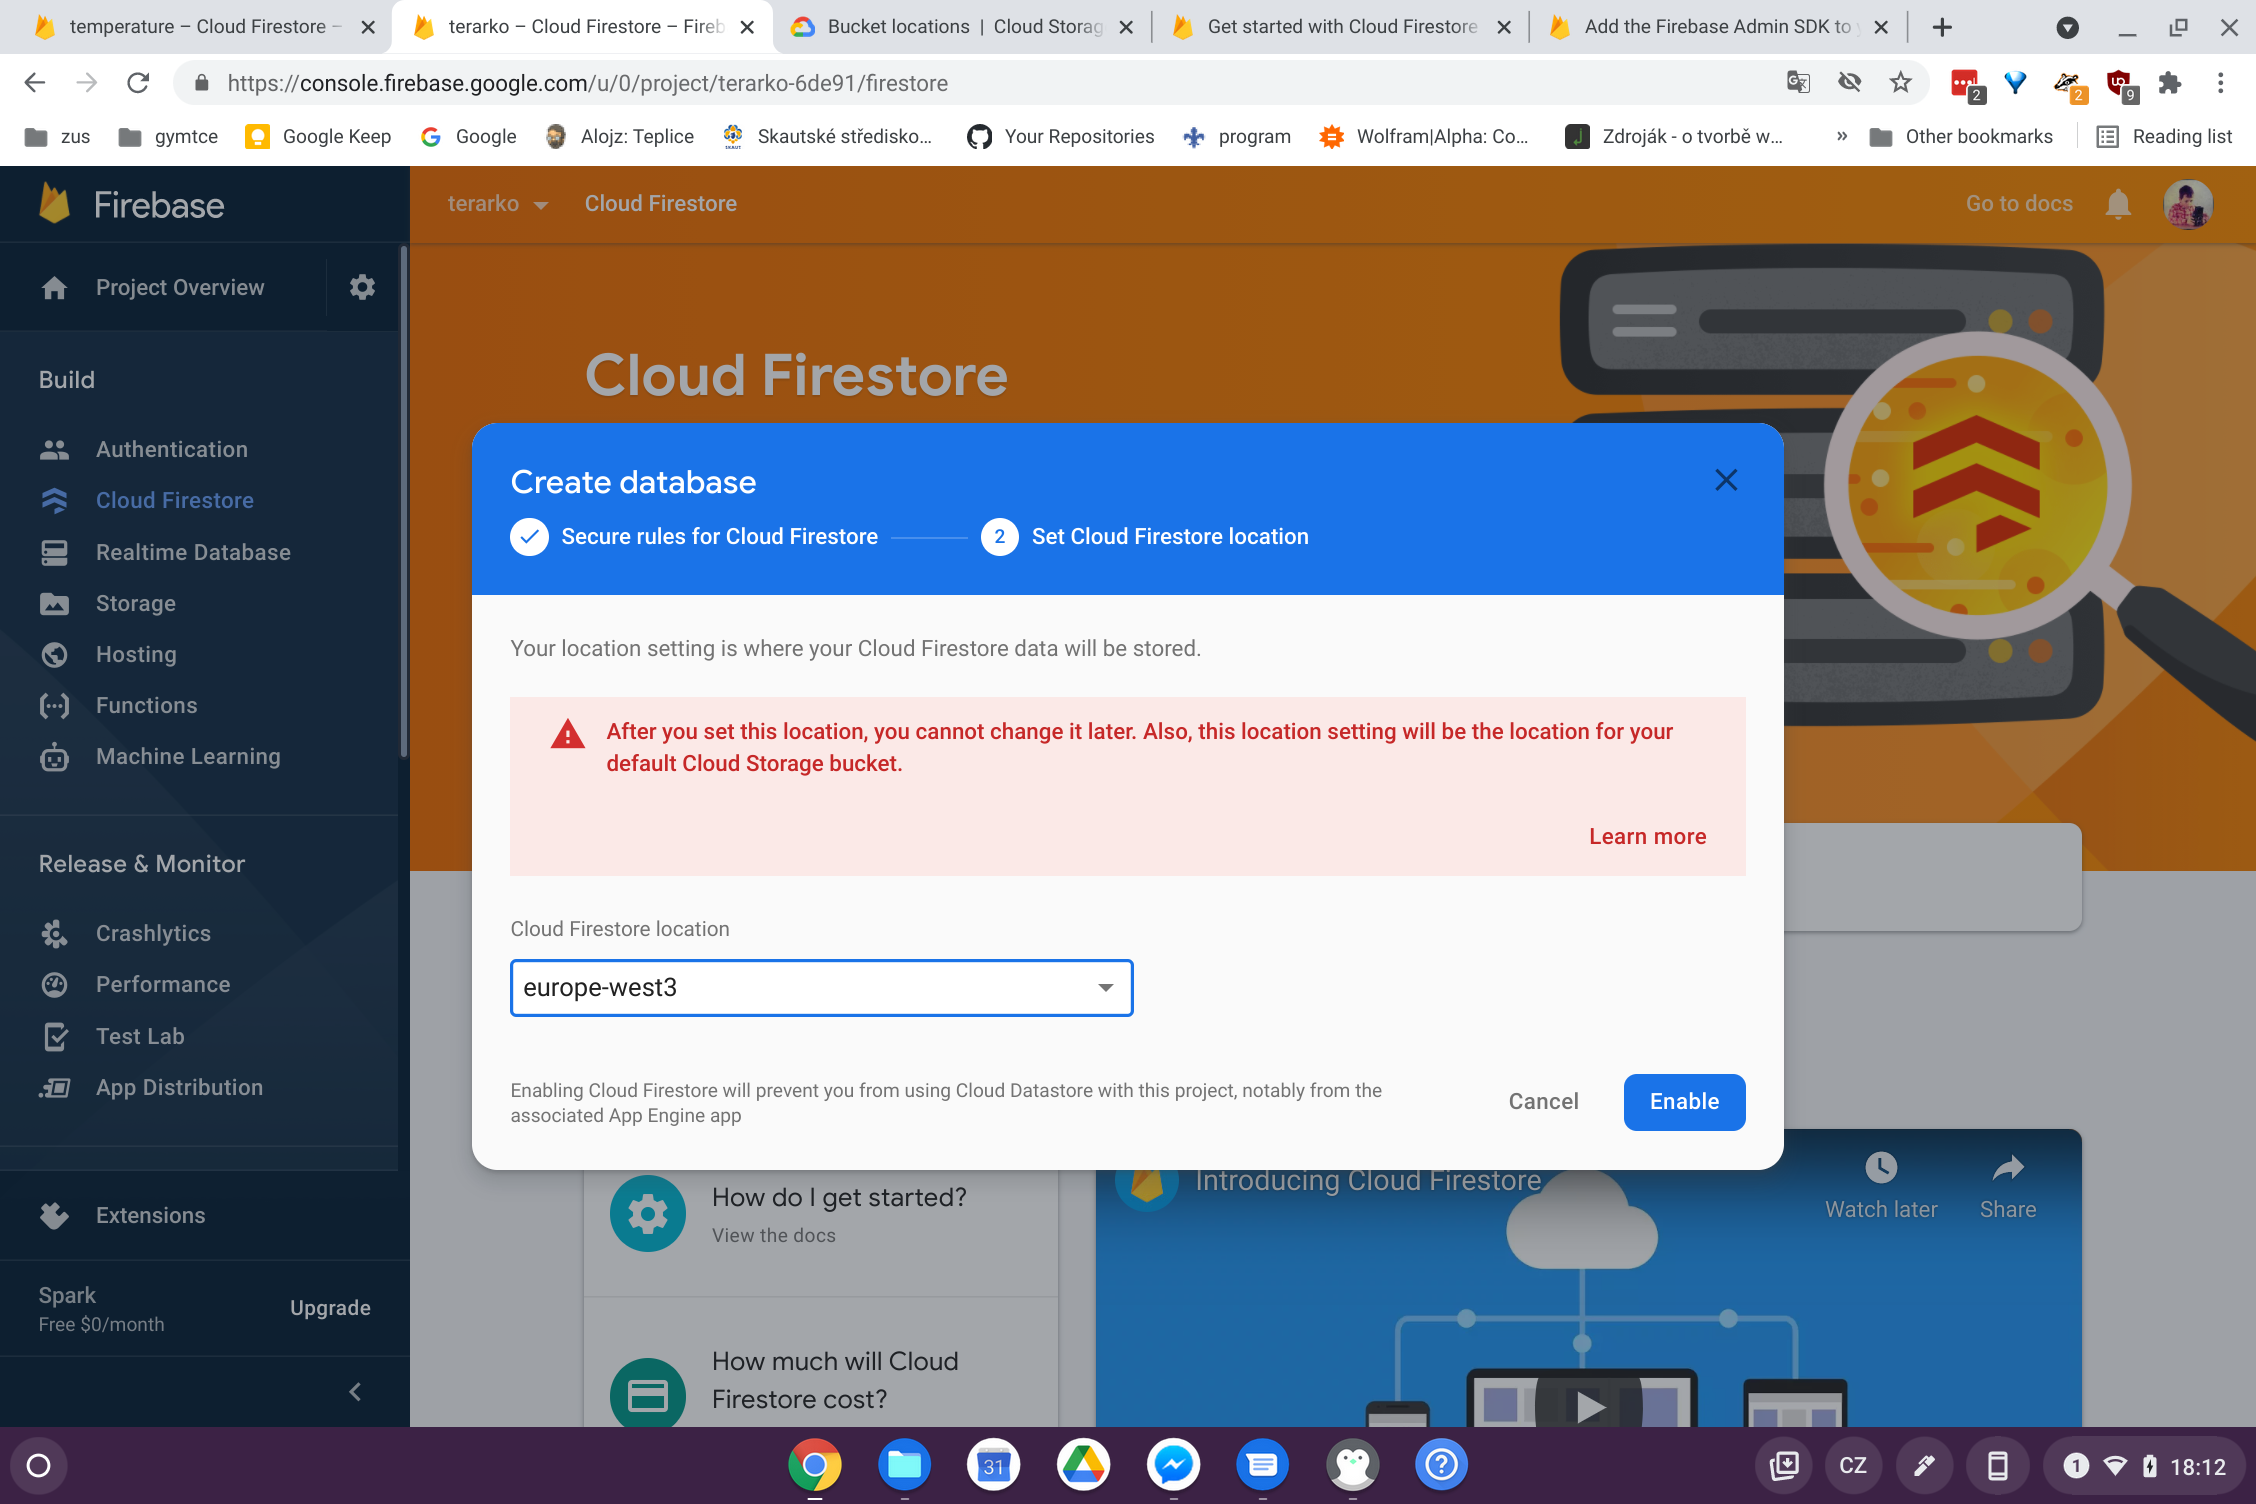
\includegraphics[width=0.8\textwidth]{firestore-2.png}
    \caption{Firestore, krok 2}
\end{figure}
Jako lokaci databáze volím Evropu konkrétně Frankfurt.
% dashboard
\begin{figure}[H]
    \centering
    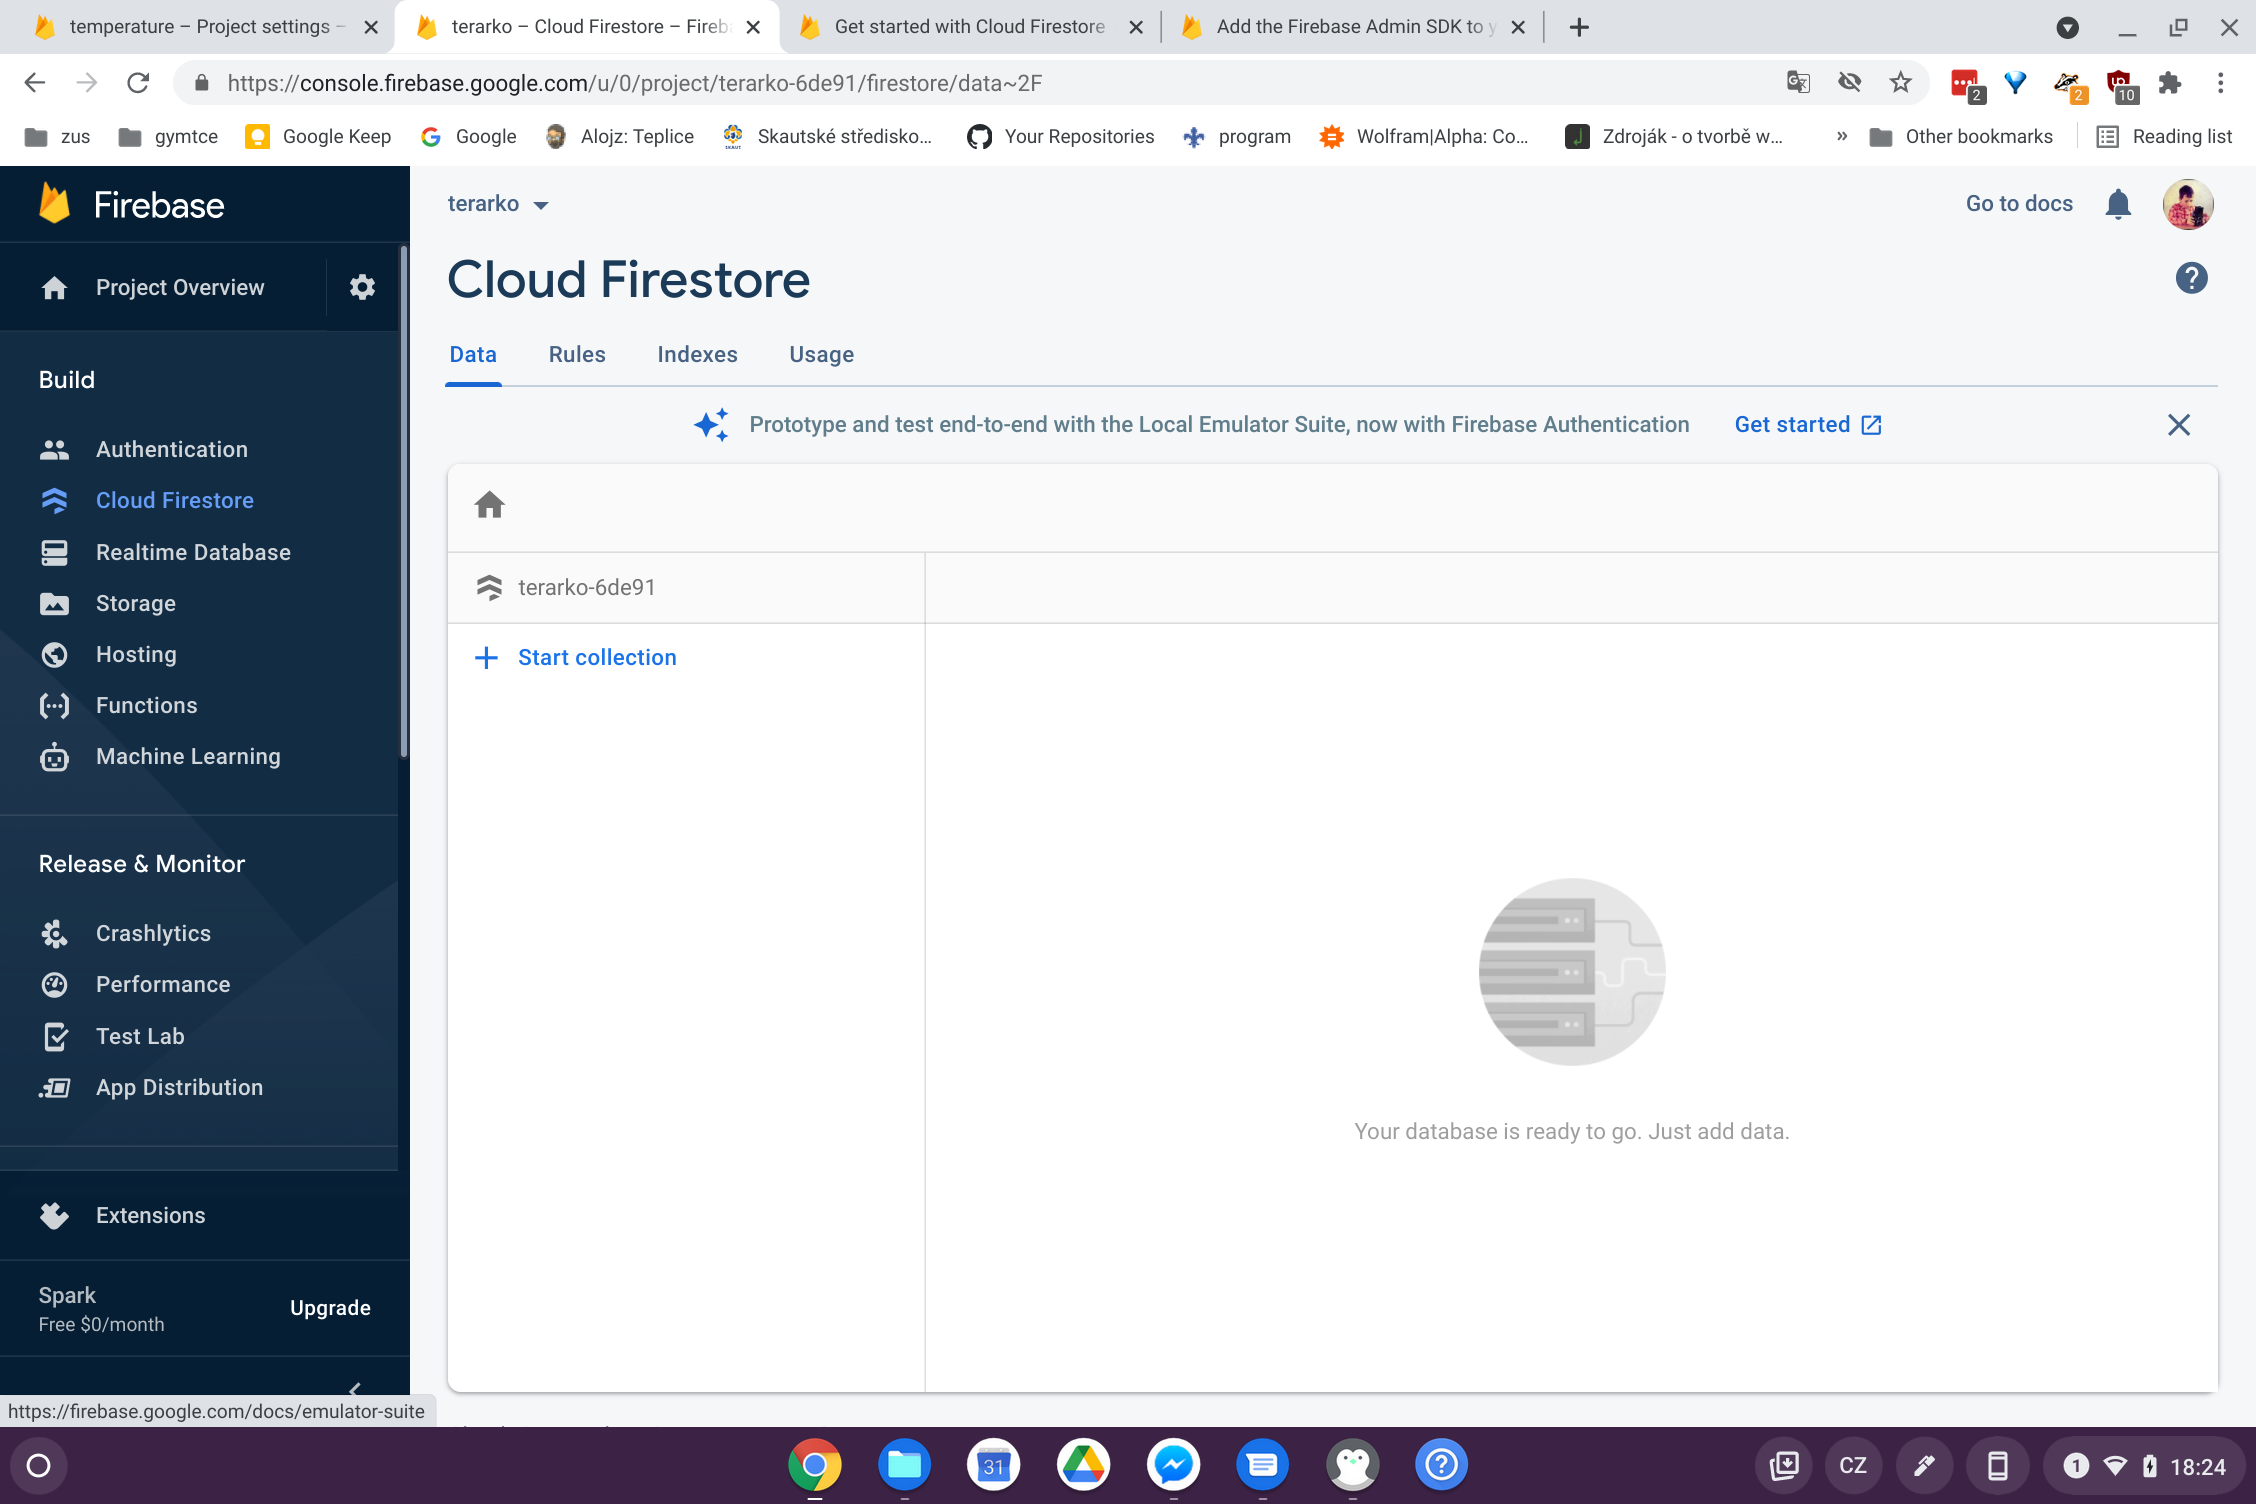
\includegraphics[width=0.8\textwidth]{firestore-dashboard.png}
    \caption{Firestore}
\end{figure}
A mám nastaveno. Teď můžu začít přidávat data.

\subsection{Hosting}
Pro \gls{hosting} jsem použil též platformu \gls{firebase}. Při založení jsem postupoval podle návodu 
(\url{https://firebase.google.com/docs/hosting}). Během inicializace jsem zvolil, že chci pouze \gls{hosting}, pro 
projekt terárko a povolil jsem \gls{github} Actions. Takže po každém commitu, který pošlu na \gls{github} se mi 
automaticky nasadí nejnovější verze stránky. Kvůli tomu jsem zdrojové kódy umístil do samostatného repozitáře.

\subsection{Webová aplikace}
Poslední co je třeba nastavit je samotná webová aplikace a její propojení s \glslink{hosting}{hostingem}. Opět znázorním 
několika obrázky.

% přidání aplikace
\begin{figure}[H]
    \centering
    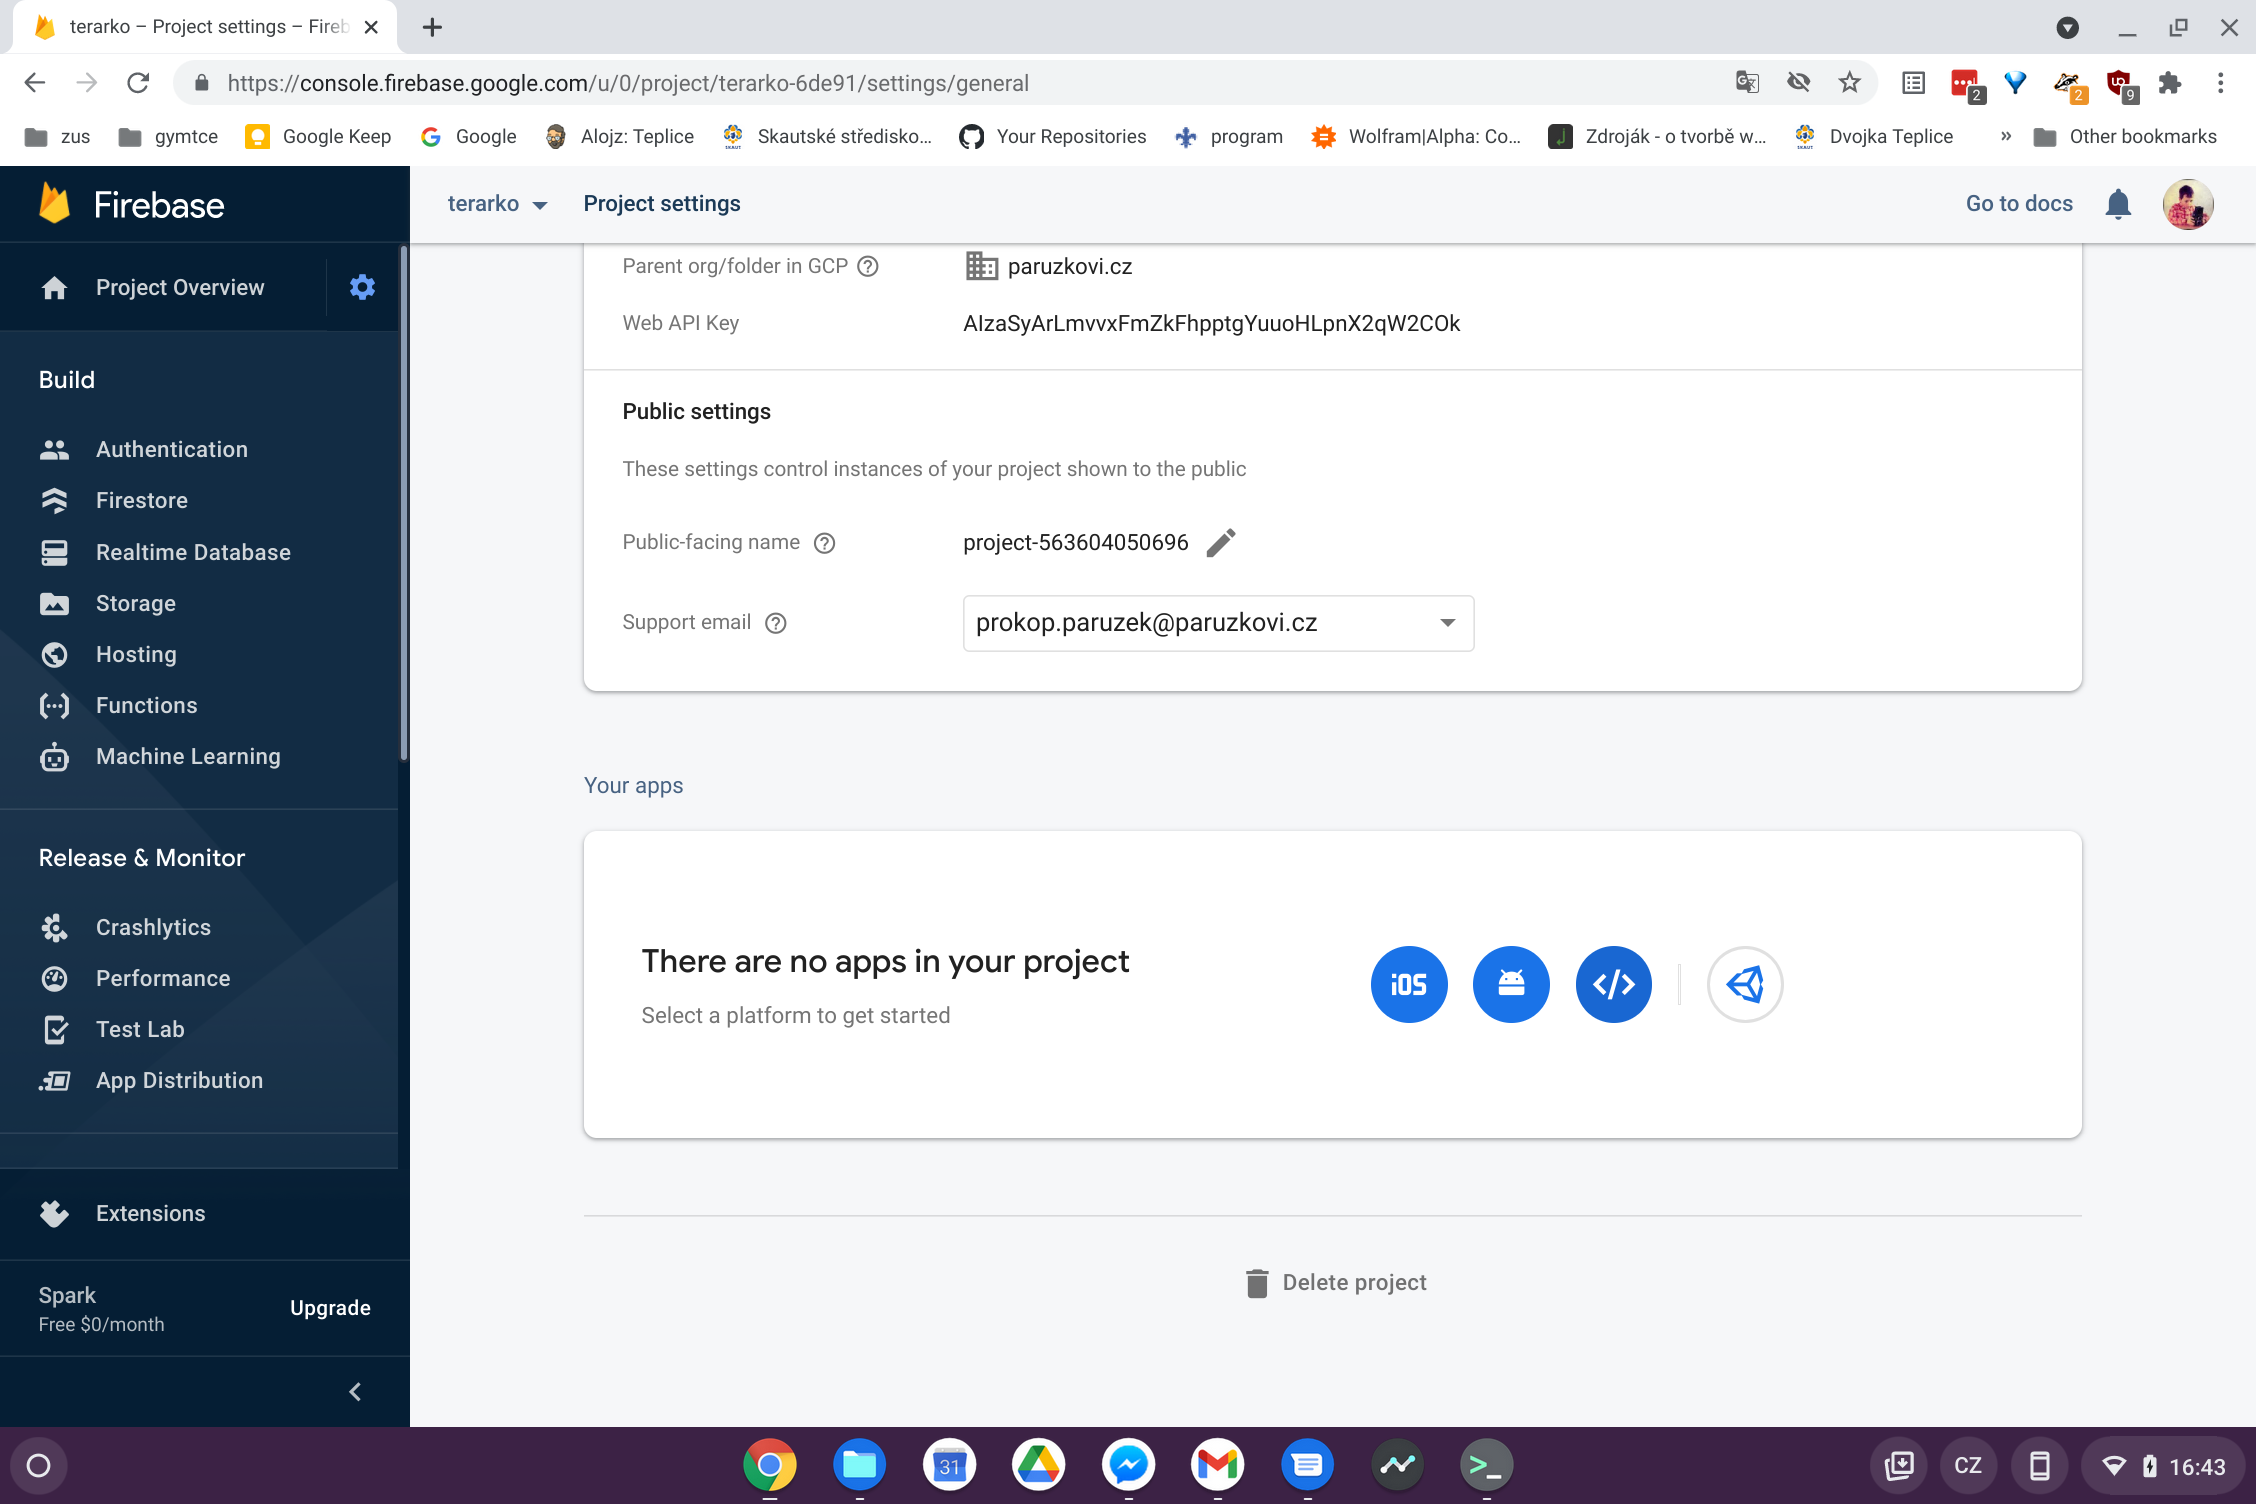
\includegraphics[width=0.8\textwidth]{firebase-addApp.png}
    \caption{Přidání aplikace}
\end{figure}
Přidávám webovou aplikaci, tj. špičaté závorky s lomítkem.
% jméno
\begin{figure}[H]
    \centering
    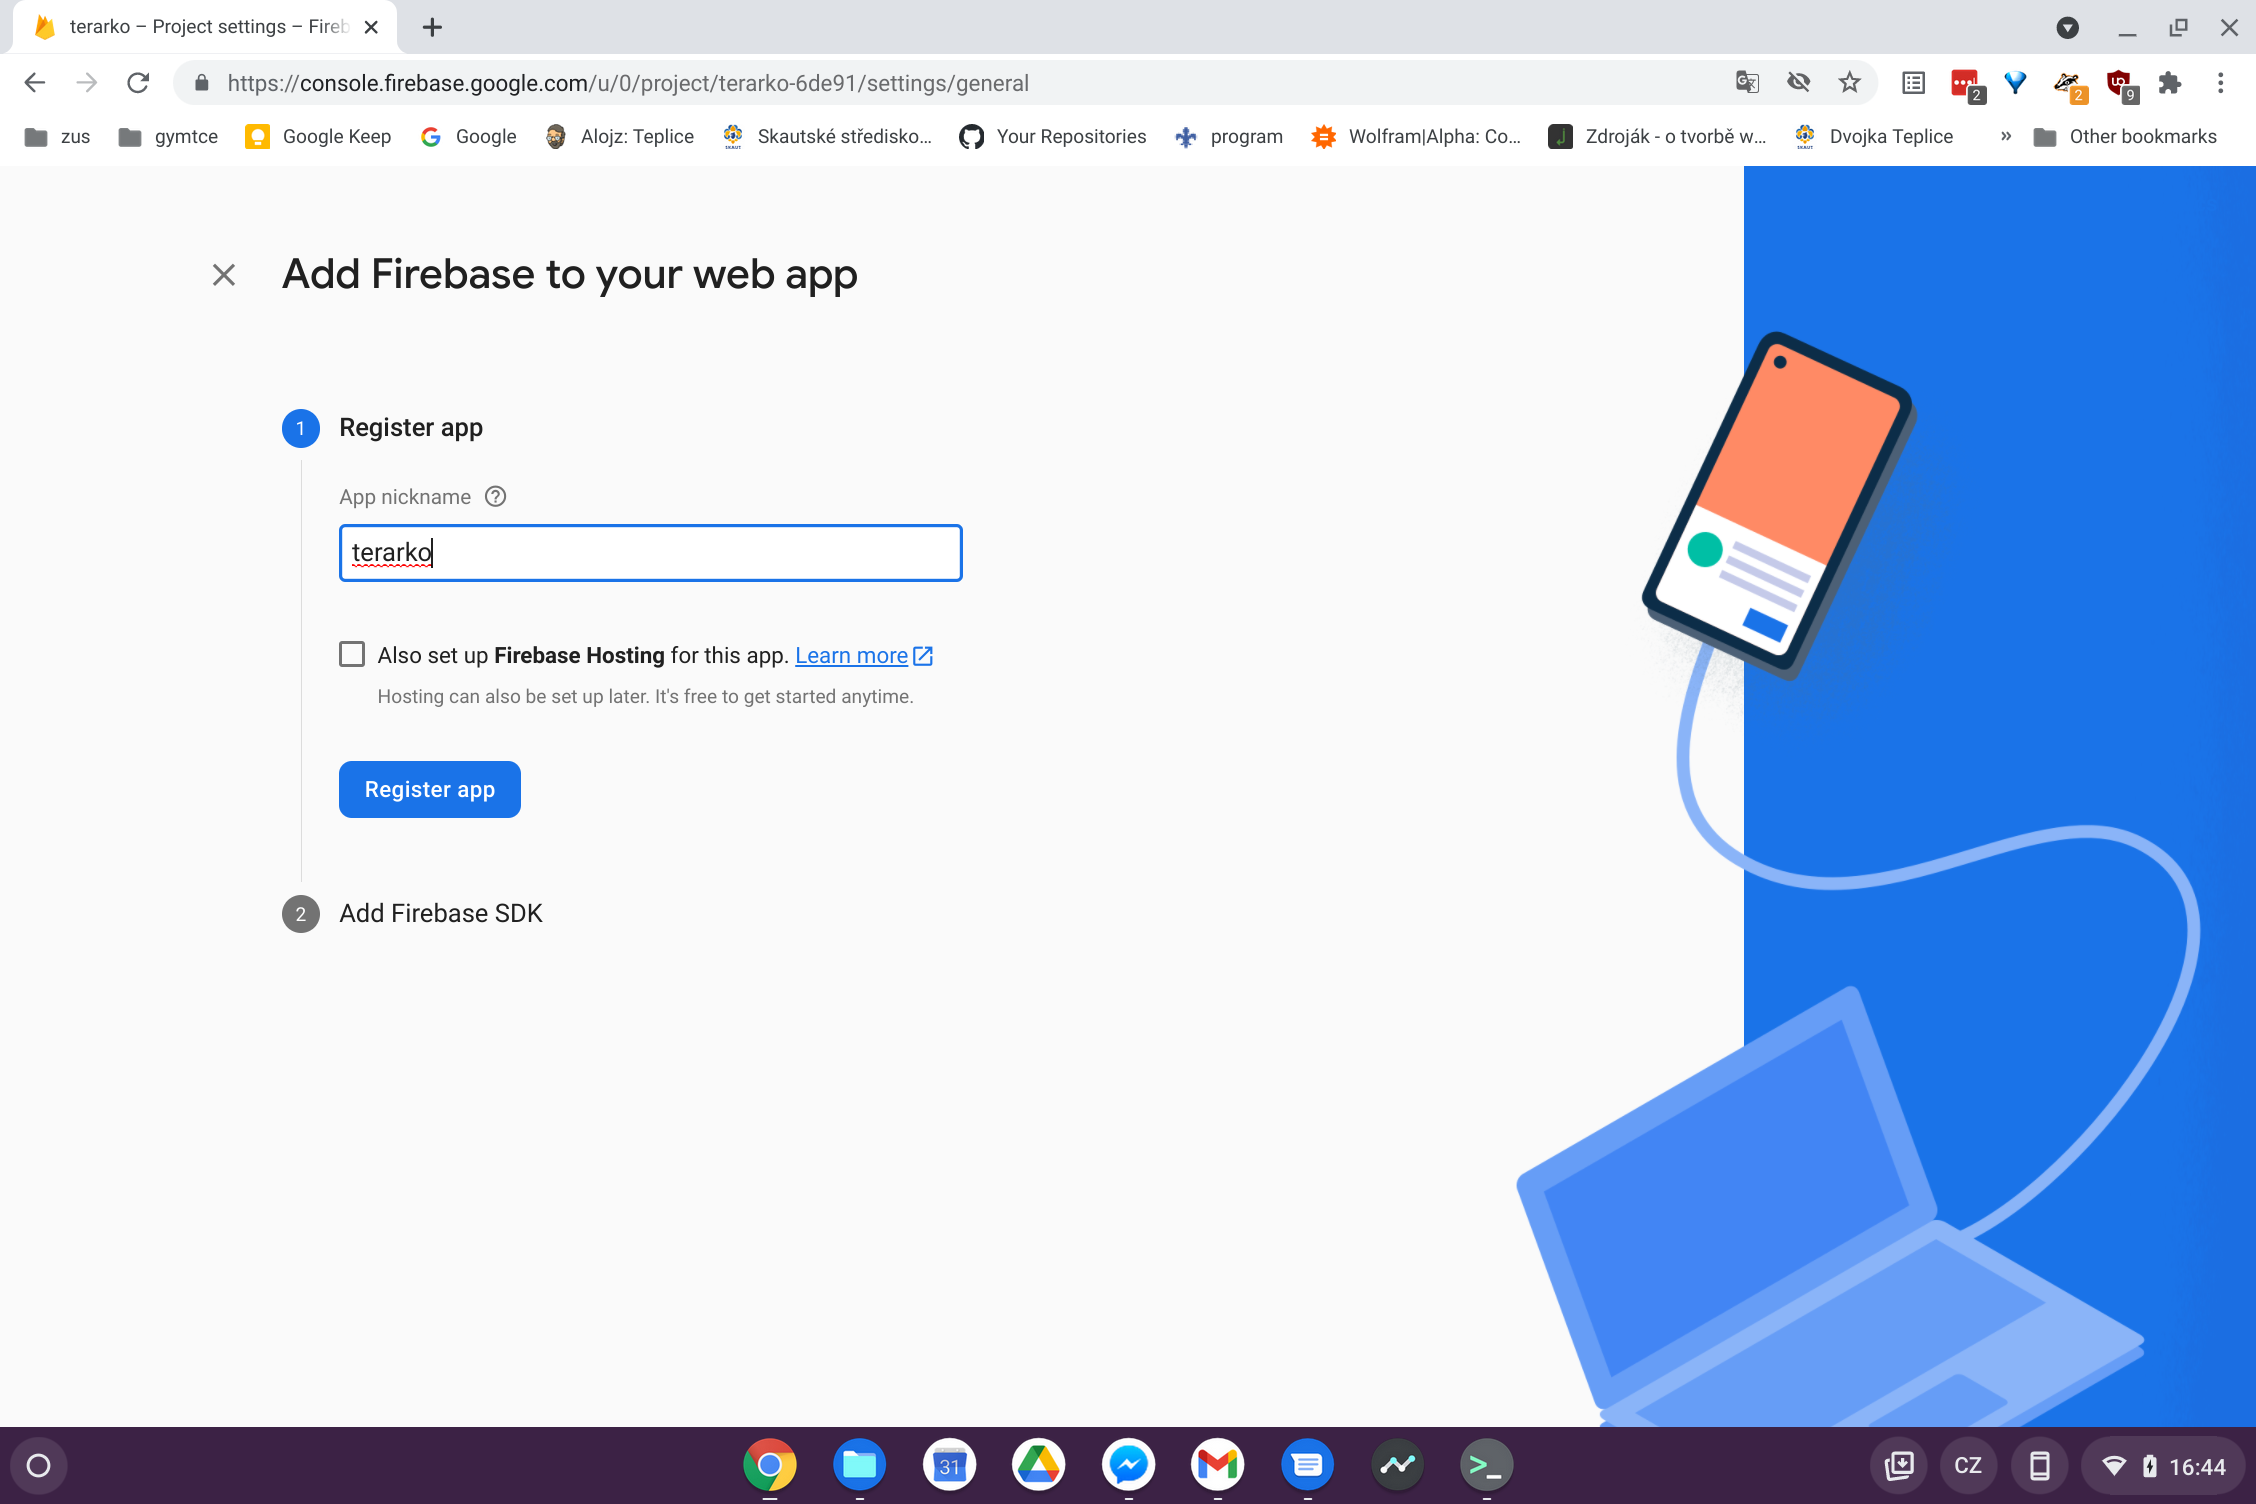
\includegraphics[width=0.8\textwidth]{firebase-app-1.png}
    \caption{Jméno aplikace}
\end{figure}
% SDK
\begin{figure}[H]
    \centering
    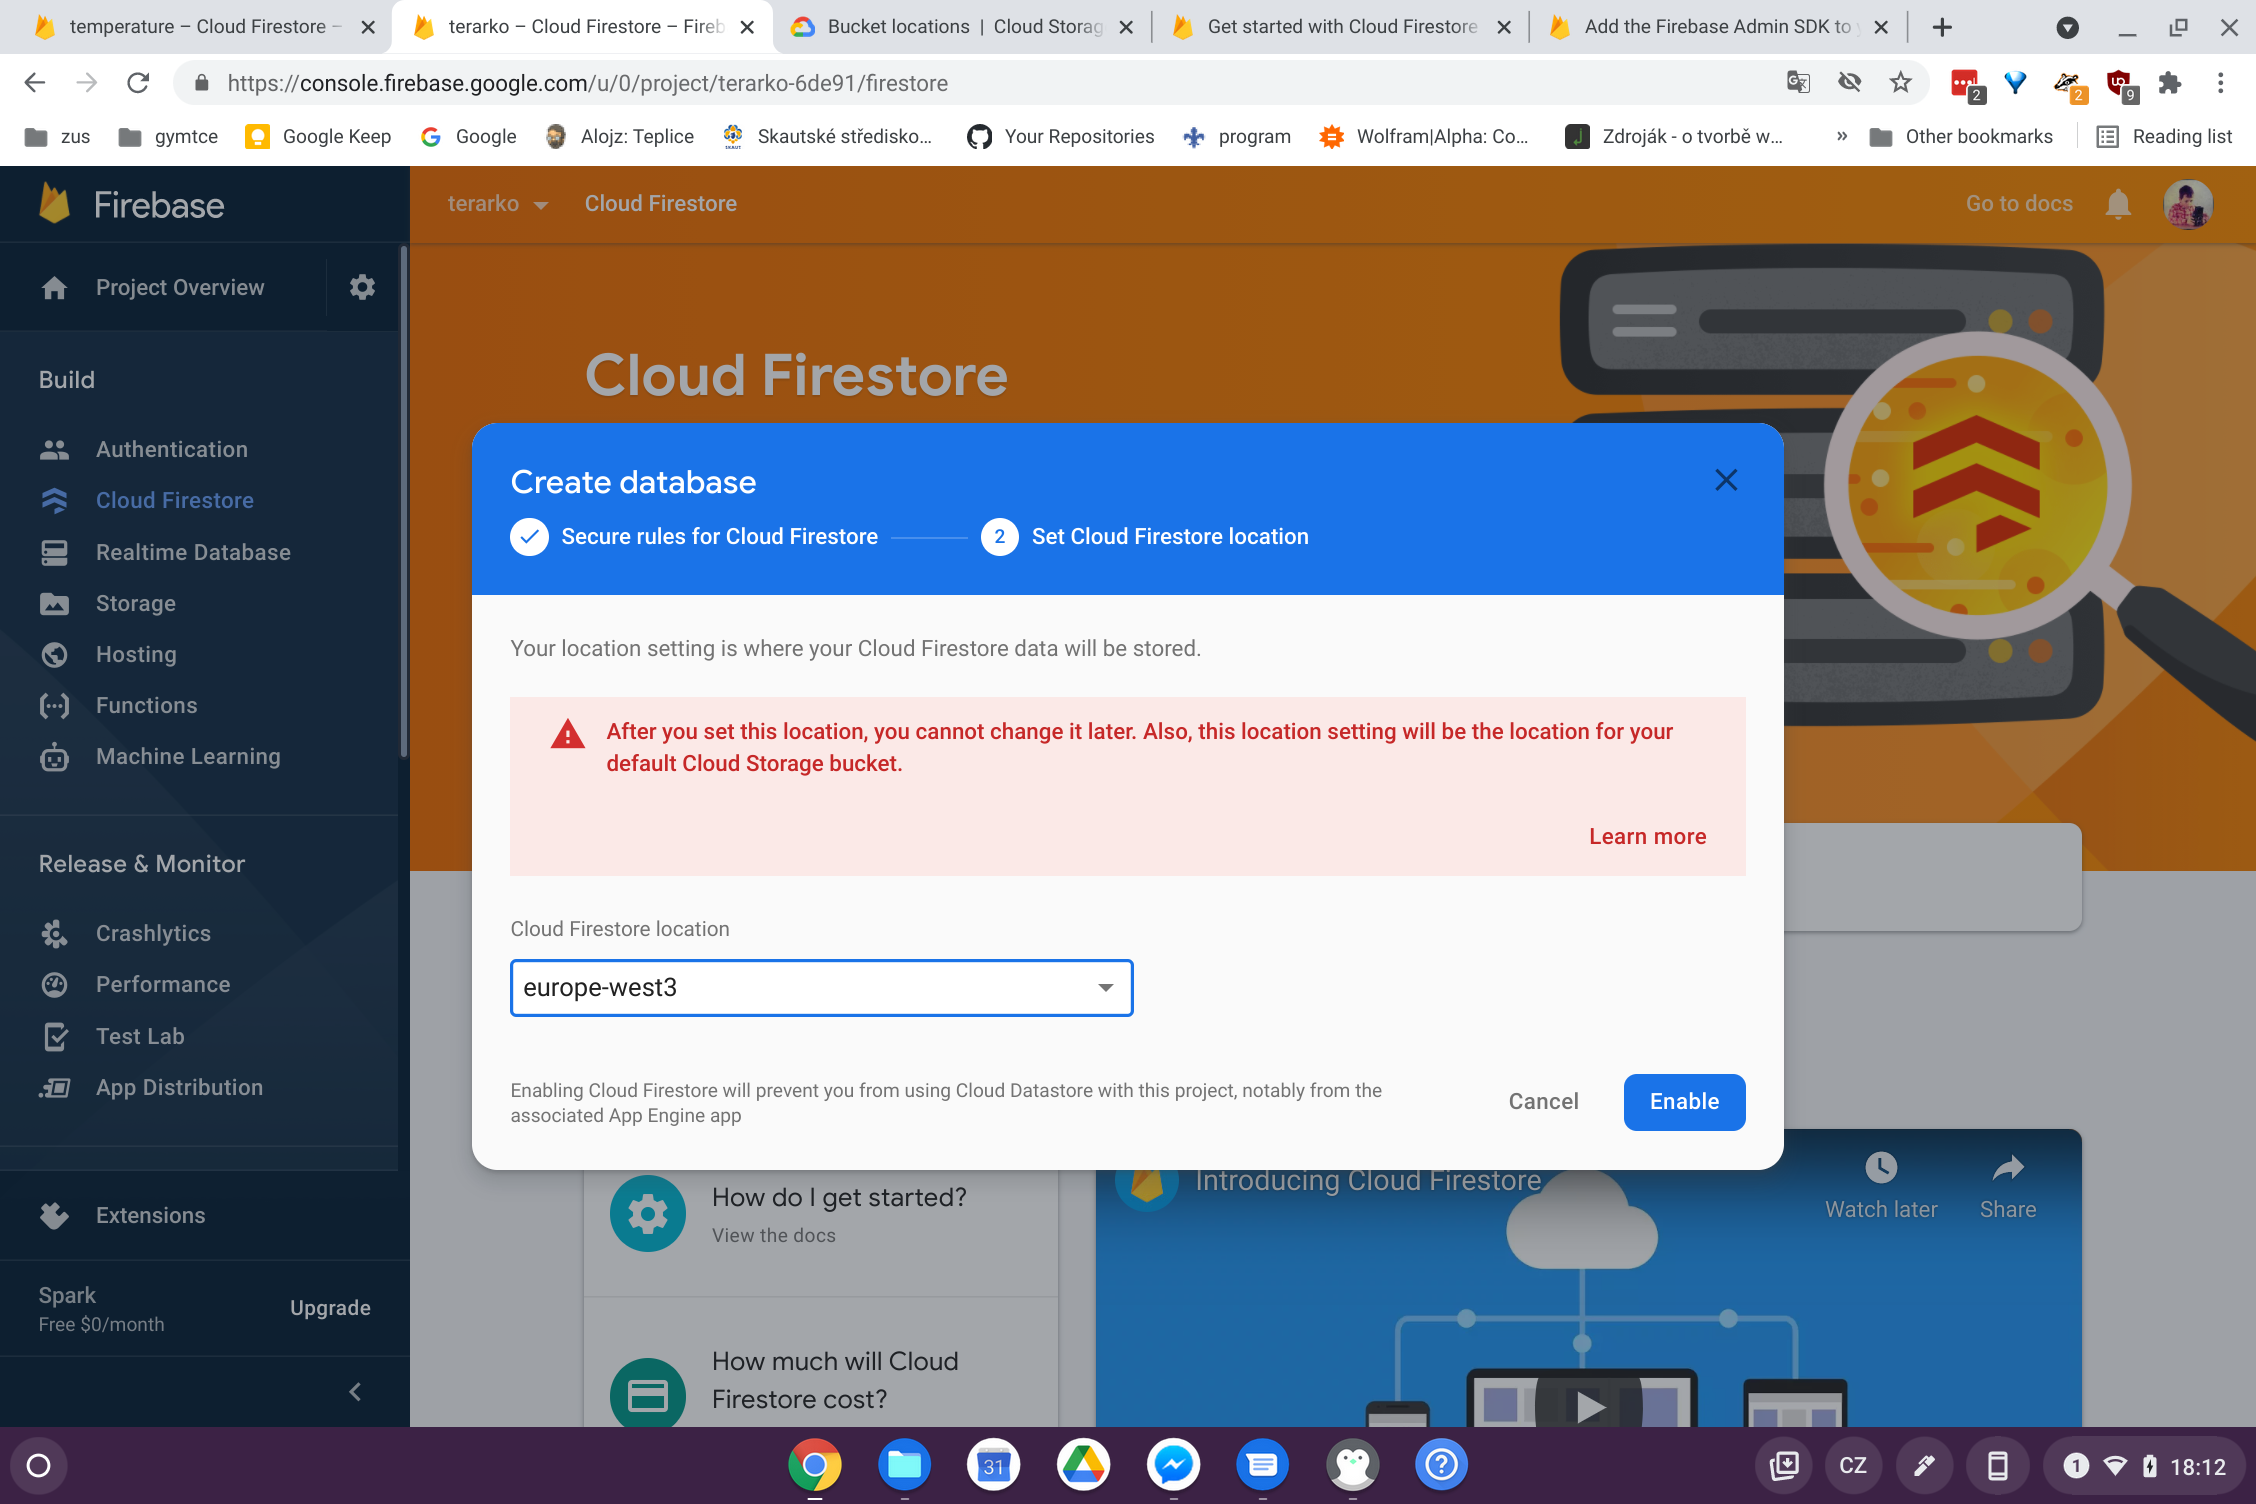
\includegraphics[width=0.8\textwidth]{firestore-2.png}
    \caption{Firestore SDK}
\end{figure}
Toto je důležité pokud si aplikaci hostujete někde u sebe. Já použiji \gls{firebase} \gls{hosting} a tudíž mi to stačí 
odkliknout.
% propojení hostingu
\begin{figure}[H]
    \centering
    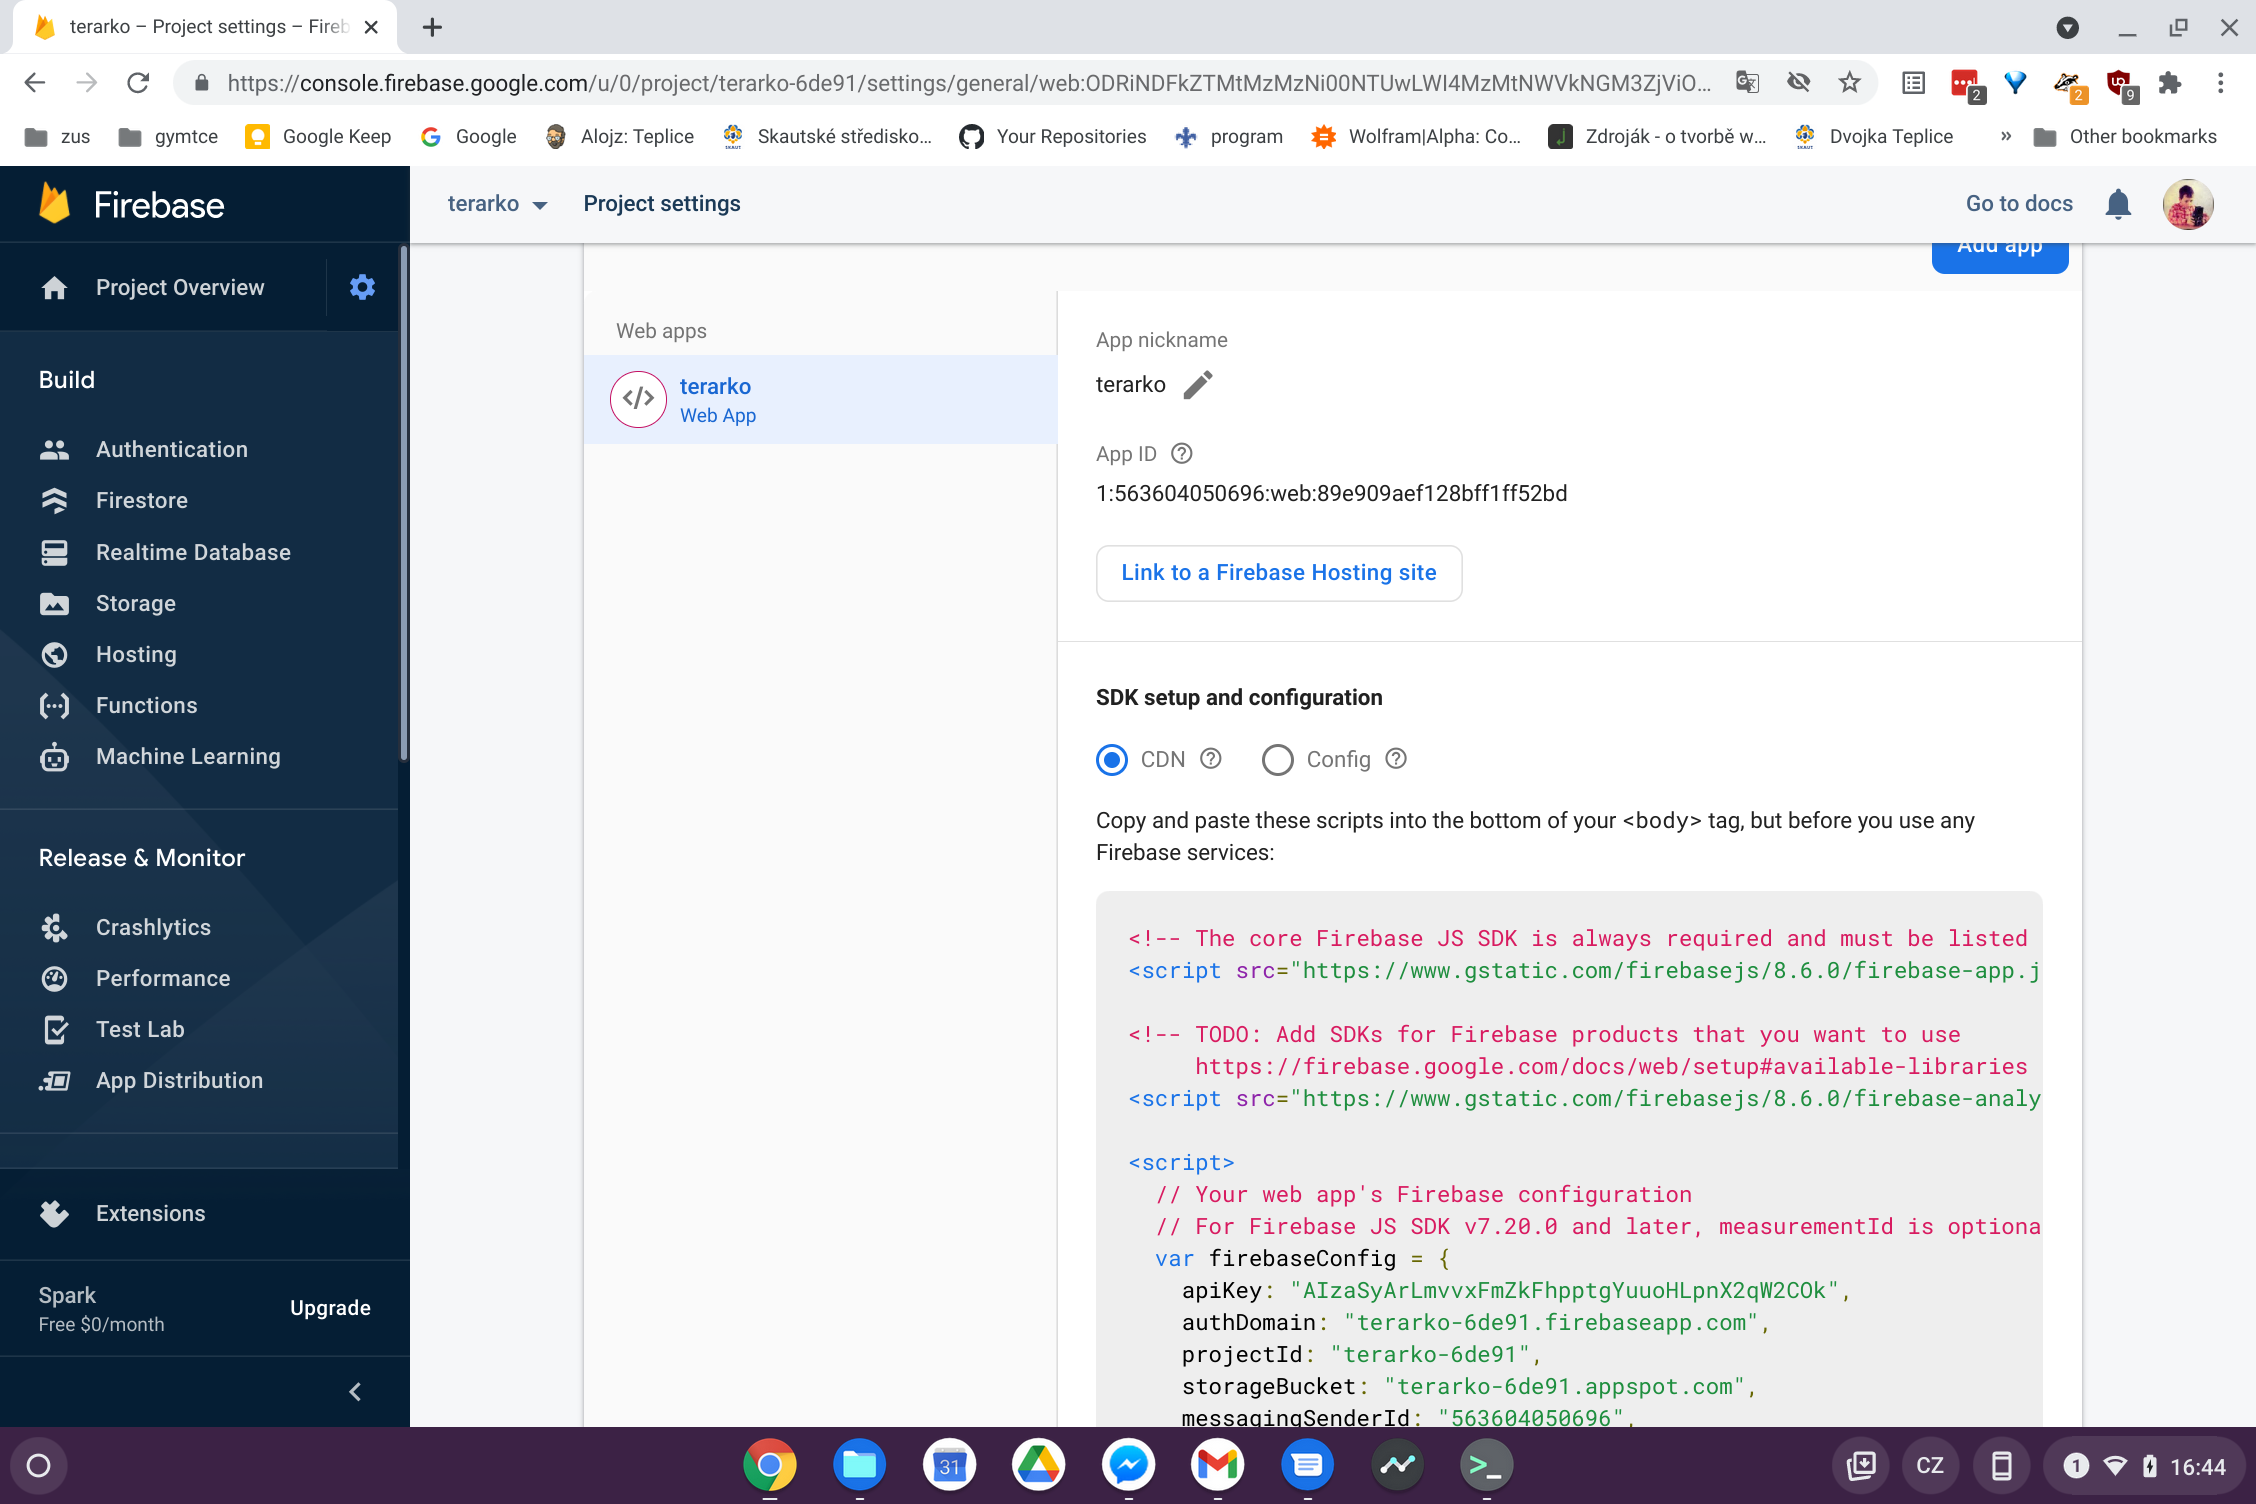
\includegraphics[width=0.8\textwidth]{firebase-app-hosting-1.png}
    \caption{Propojení s hostingem}
\end{figure}
Nyní chci propojit aplikaci s firebase \glslink{hosting}{hostingu}.
% vybrání hostingu
\begin{figure}[H]
    \centering
    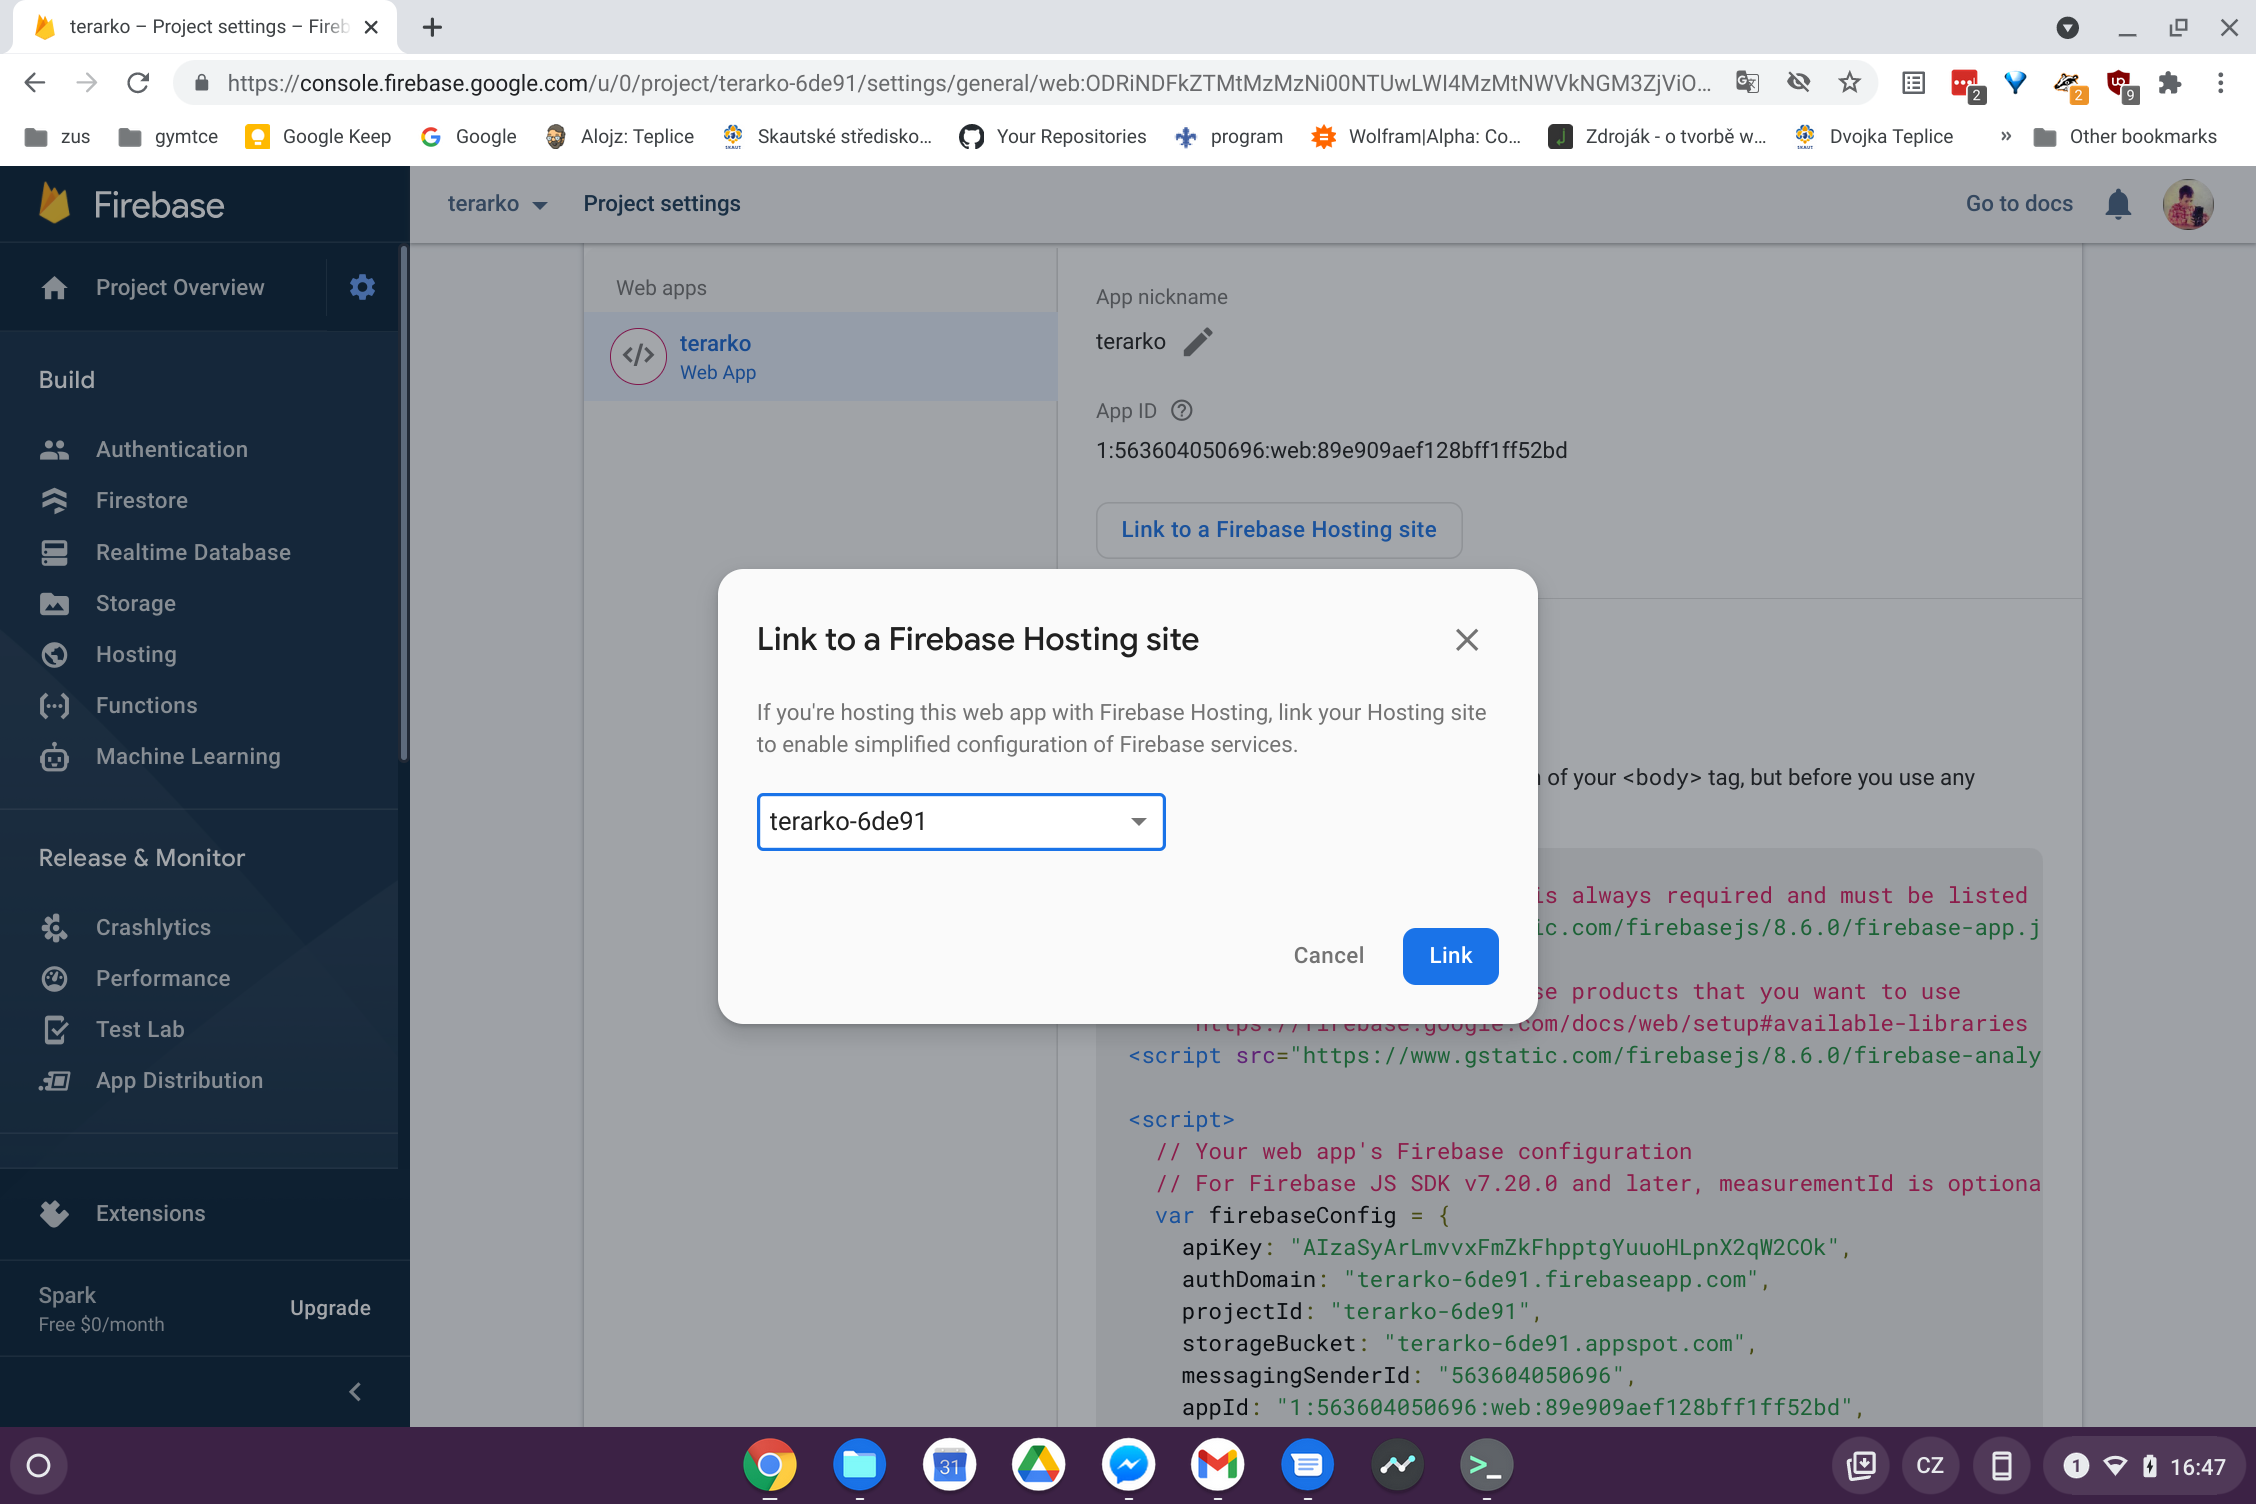
\includegraphics[width=0.8\textwidth]{firebase-app-hosting-2.png}
    \caption{Vybrání hostingu}
\end{figure}
Zde vyberu jaký \gls{hosting} chci použít a to mi umožní zjednodušit kód stránek, protože si všechny ty konfigurační 
údaje načte přímo z \glslink{hosting}{hostingu} spolu s \gls{firebase} \glslink{knihovna}{knihovnami}.
\begin{figure}[H]
    \centering
    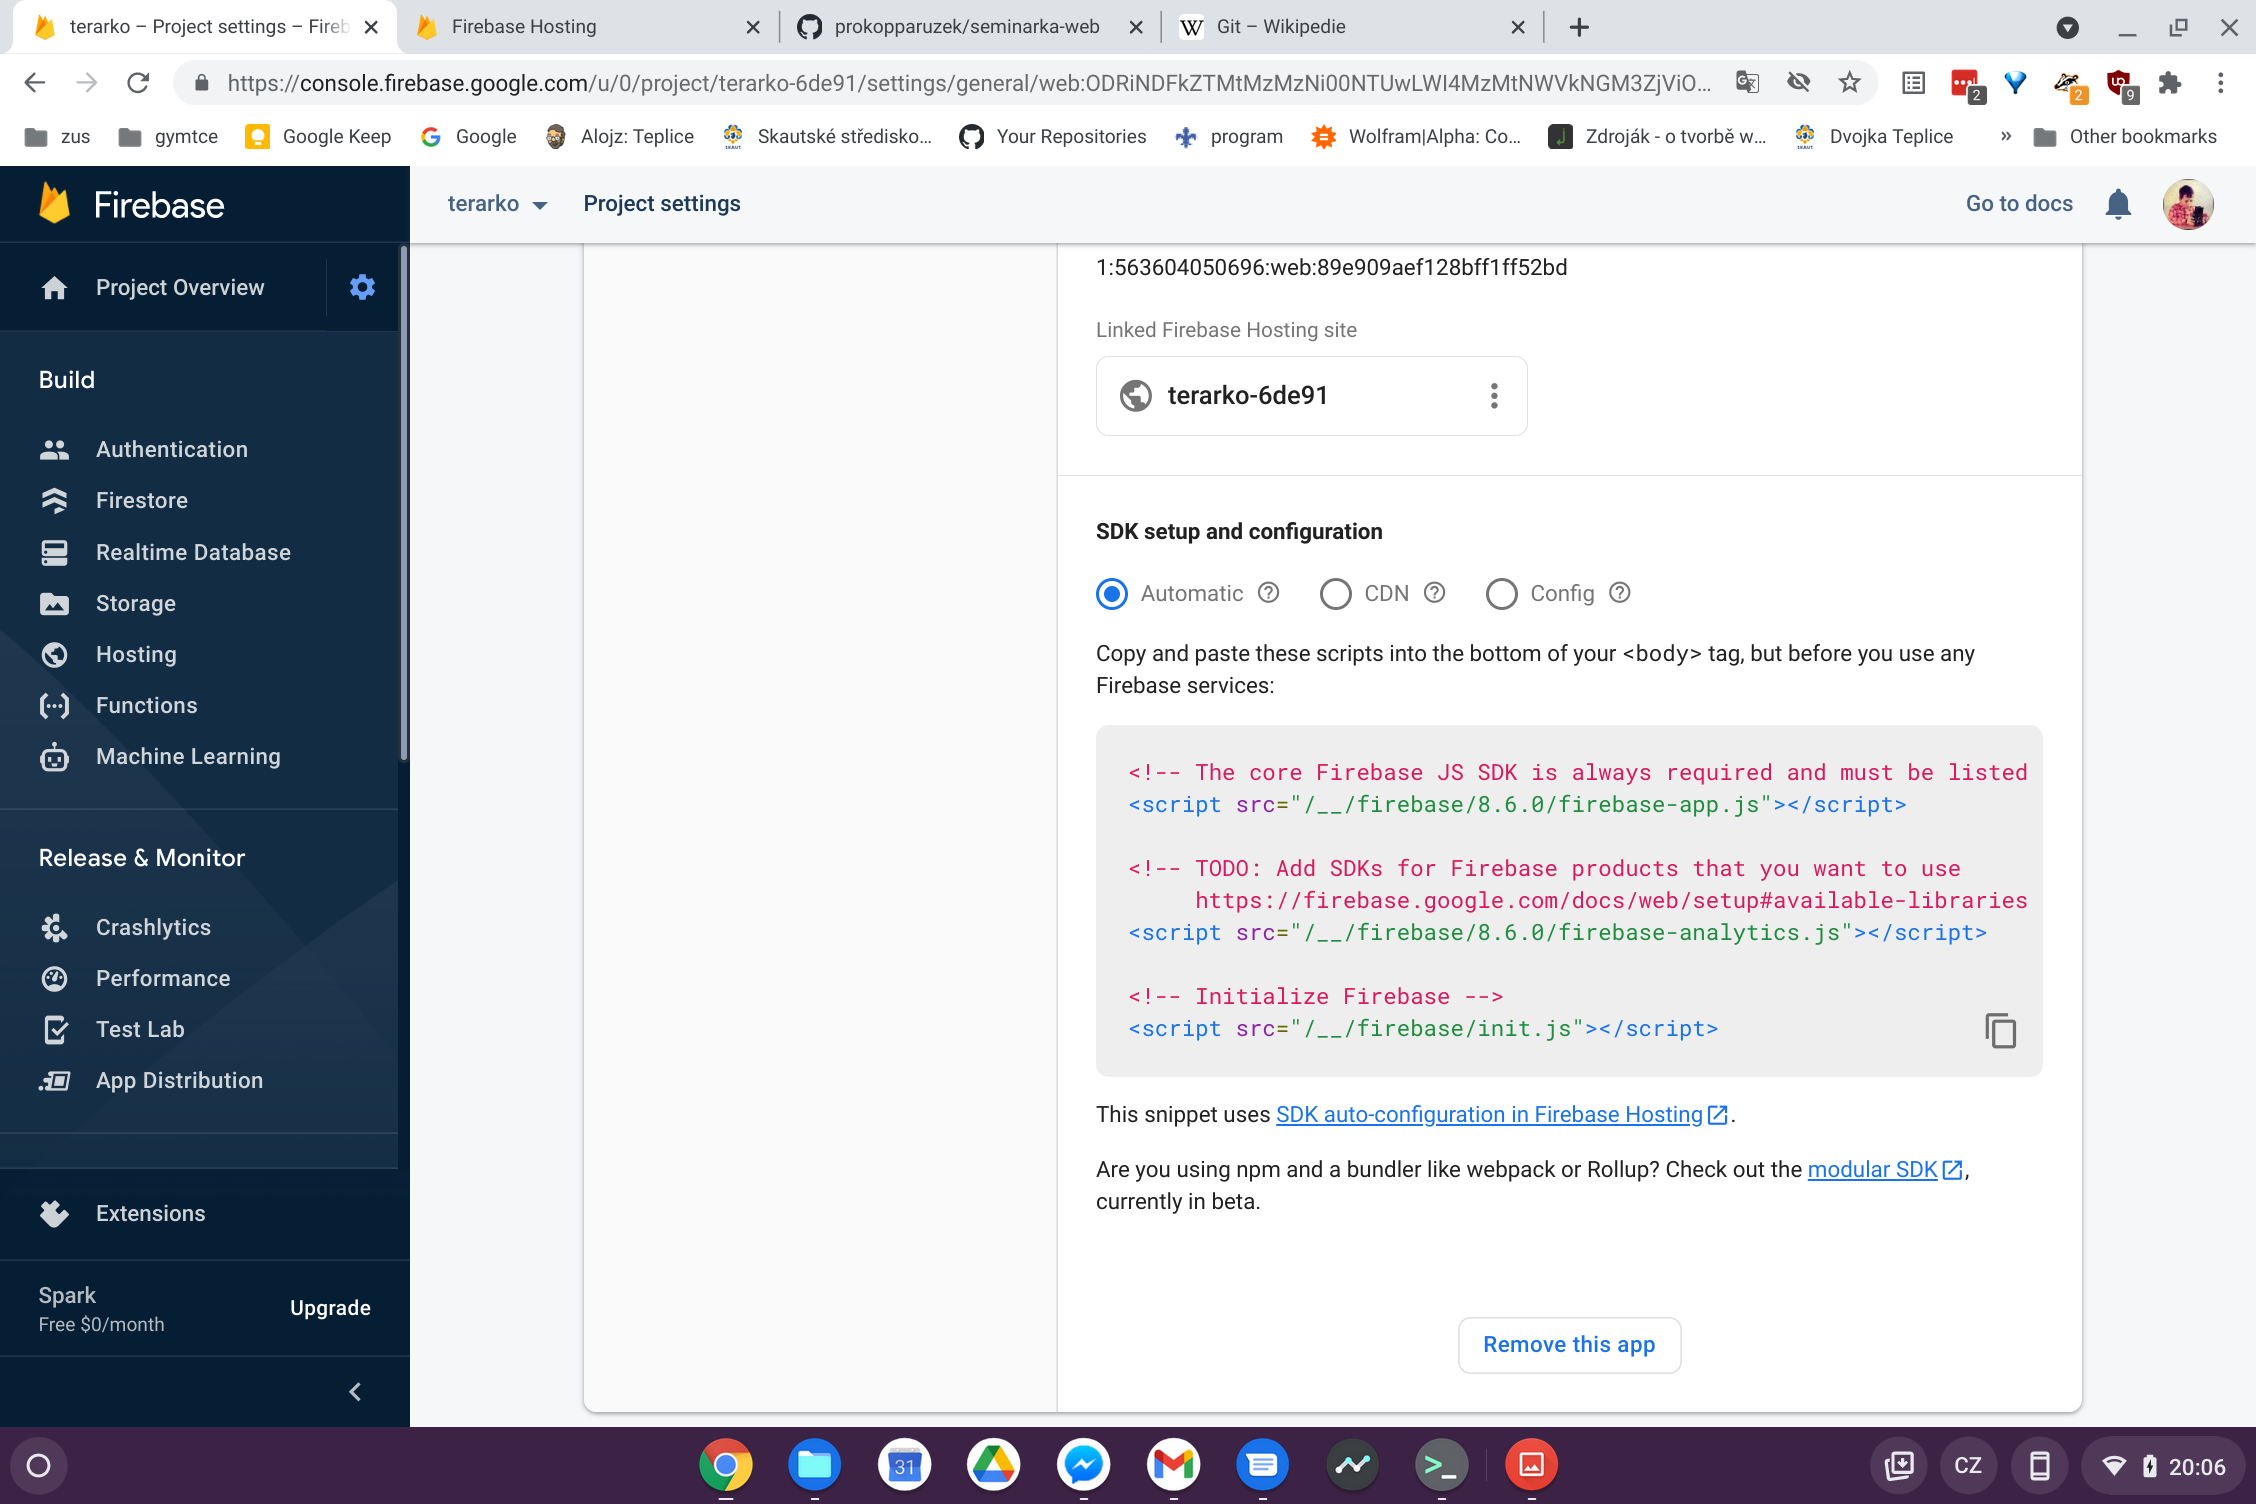
\includegraphics[width=0.8\textwidth]{firebase-app-hosting-3.png}
    \caption{Zjednodušený kód}
\end{figure}
Zde je vidět jak z mnoha řádků kódu zbyly pouze tři při využití \gls{firebase} \glslink{hosting}{hostingu}.

\section{Domácí gateway}
% úvod
Domácí brána je v podstatě velmi jednoduchý program, který pouze přeposílá data, jež obdrží od NATS serveru, do 
\gls{firebase} Firestoru. Z důvodů popsaných výše jsem jako jazyk opět zvolil \gls{go}.

% graf
\begin{figure}[H]
    \centering
    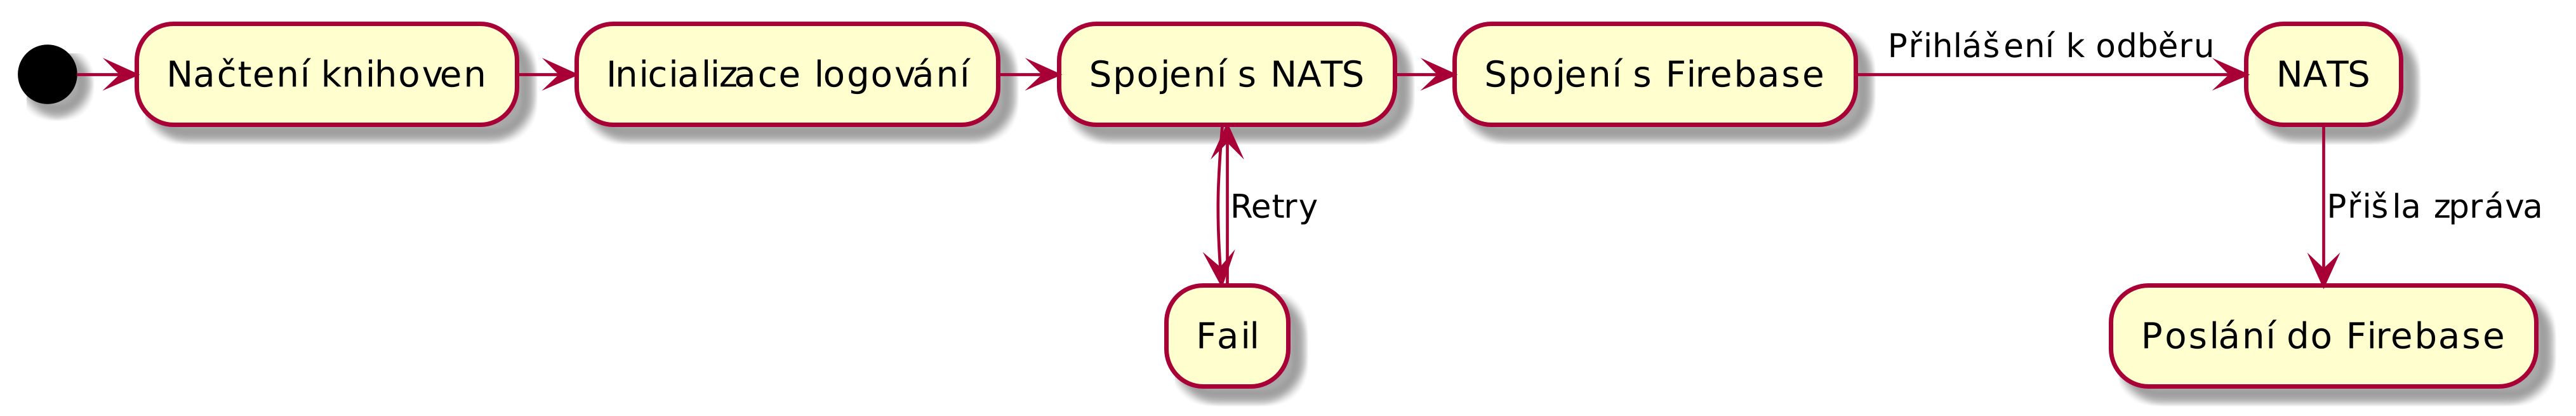
\includegraphics[width=\textwidth]{gateway.png}
    \caption{Průběh programu}
\end{figure}

% sběr informací
Spojení s NATSem je stejné jako u odesílání dat. Jediný rozdíl je v aplikační části, kdy data neodesílám, ale přijímám. 
Příjem probíhá tak, že se přihlásím k odběru kanálu, do kterého měřící stanice odesílá data a pro každou zprávu, která 
přijde spustím funkci, která ji pošle dál. Trochu nestandardní je přihlášení k odběru. Používám takzvanou \uv{durable 
subscription}. Jedná se o funkci NATS streaming serveru, která mi umožňuje přihlásit se pod určitým jménem a server si 
pak pamatuje, jakou poslední zprávu mi posílal. Takže když dojde k výpadku, po opětovném připojení mi pošle všechny 
zprávy, které jsem dosud nedostal \parencite{root.cz:NATS-streaming}.

% odesílání do cloudu
Jediné co funkce zpracovávající naměřená data dělá, je přeposílání do cloudu. Celou komunikaci s cloudem jsem v podstatě 
opsal z dokumentace firestoru (\url{https://firebase.google.com/docs/firestore}). Začíná to inicializací spojení. 
Přihlašování probíhá přes vygenerovaný soubor s privátním klíčem. Soubor jsem pouze stáhnul, uložil někam, kde k němu má 
aplikace přístup, a řekl jsem jí, kde ho má hledat. O zbytek se postará Googlem poskytovaná \gls{knihovna}. To proběhne 
po startu programu, a pak se vytvořené spojení používá až do konce. Poté už se jen přeposílají data.

% krok 1
\begin{figure}[H]
    \centering
    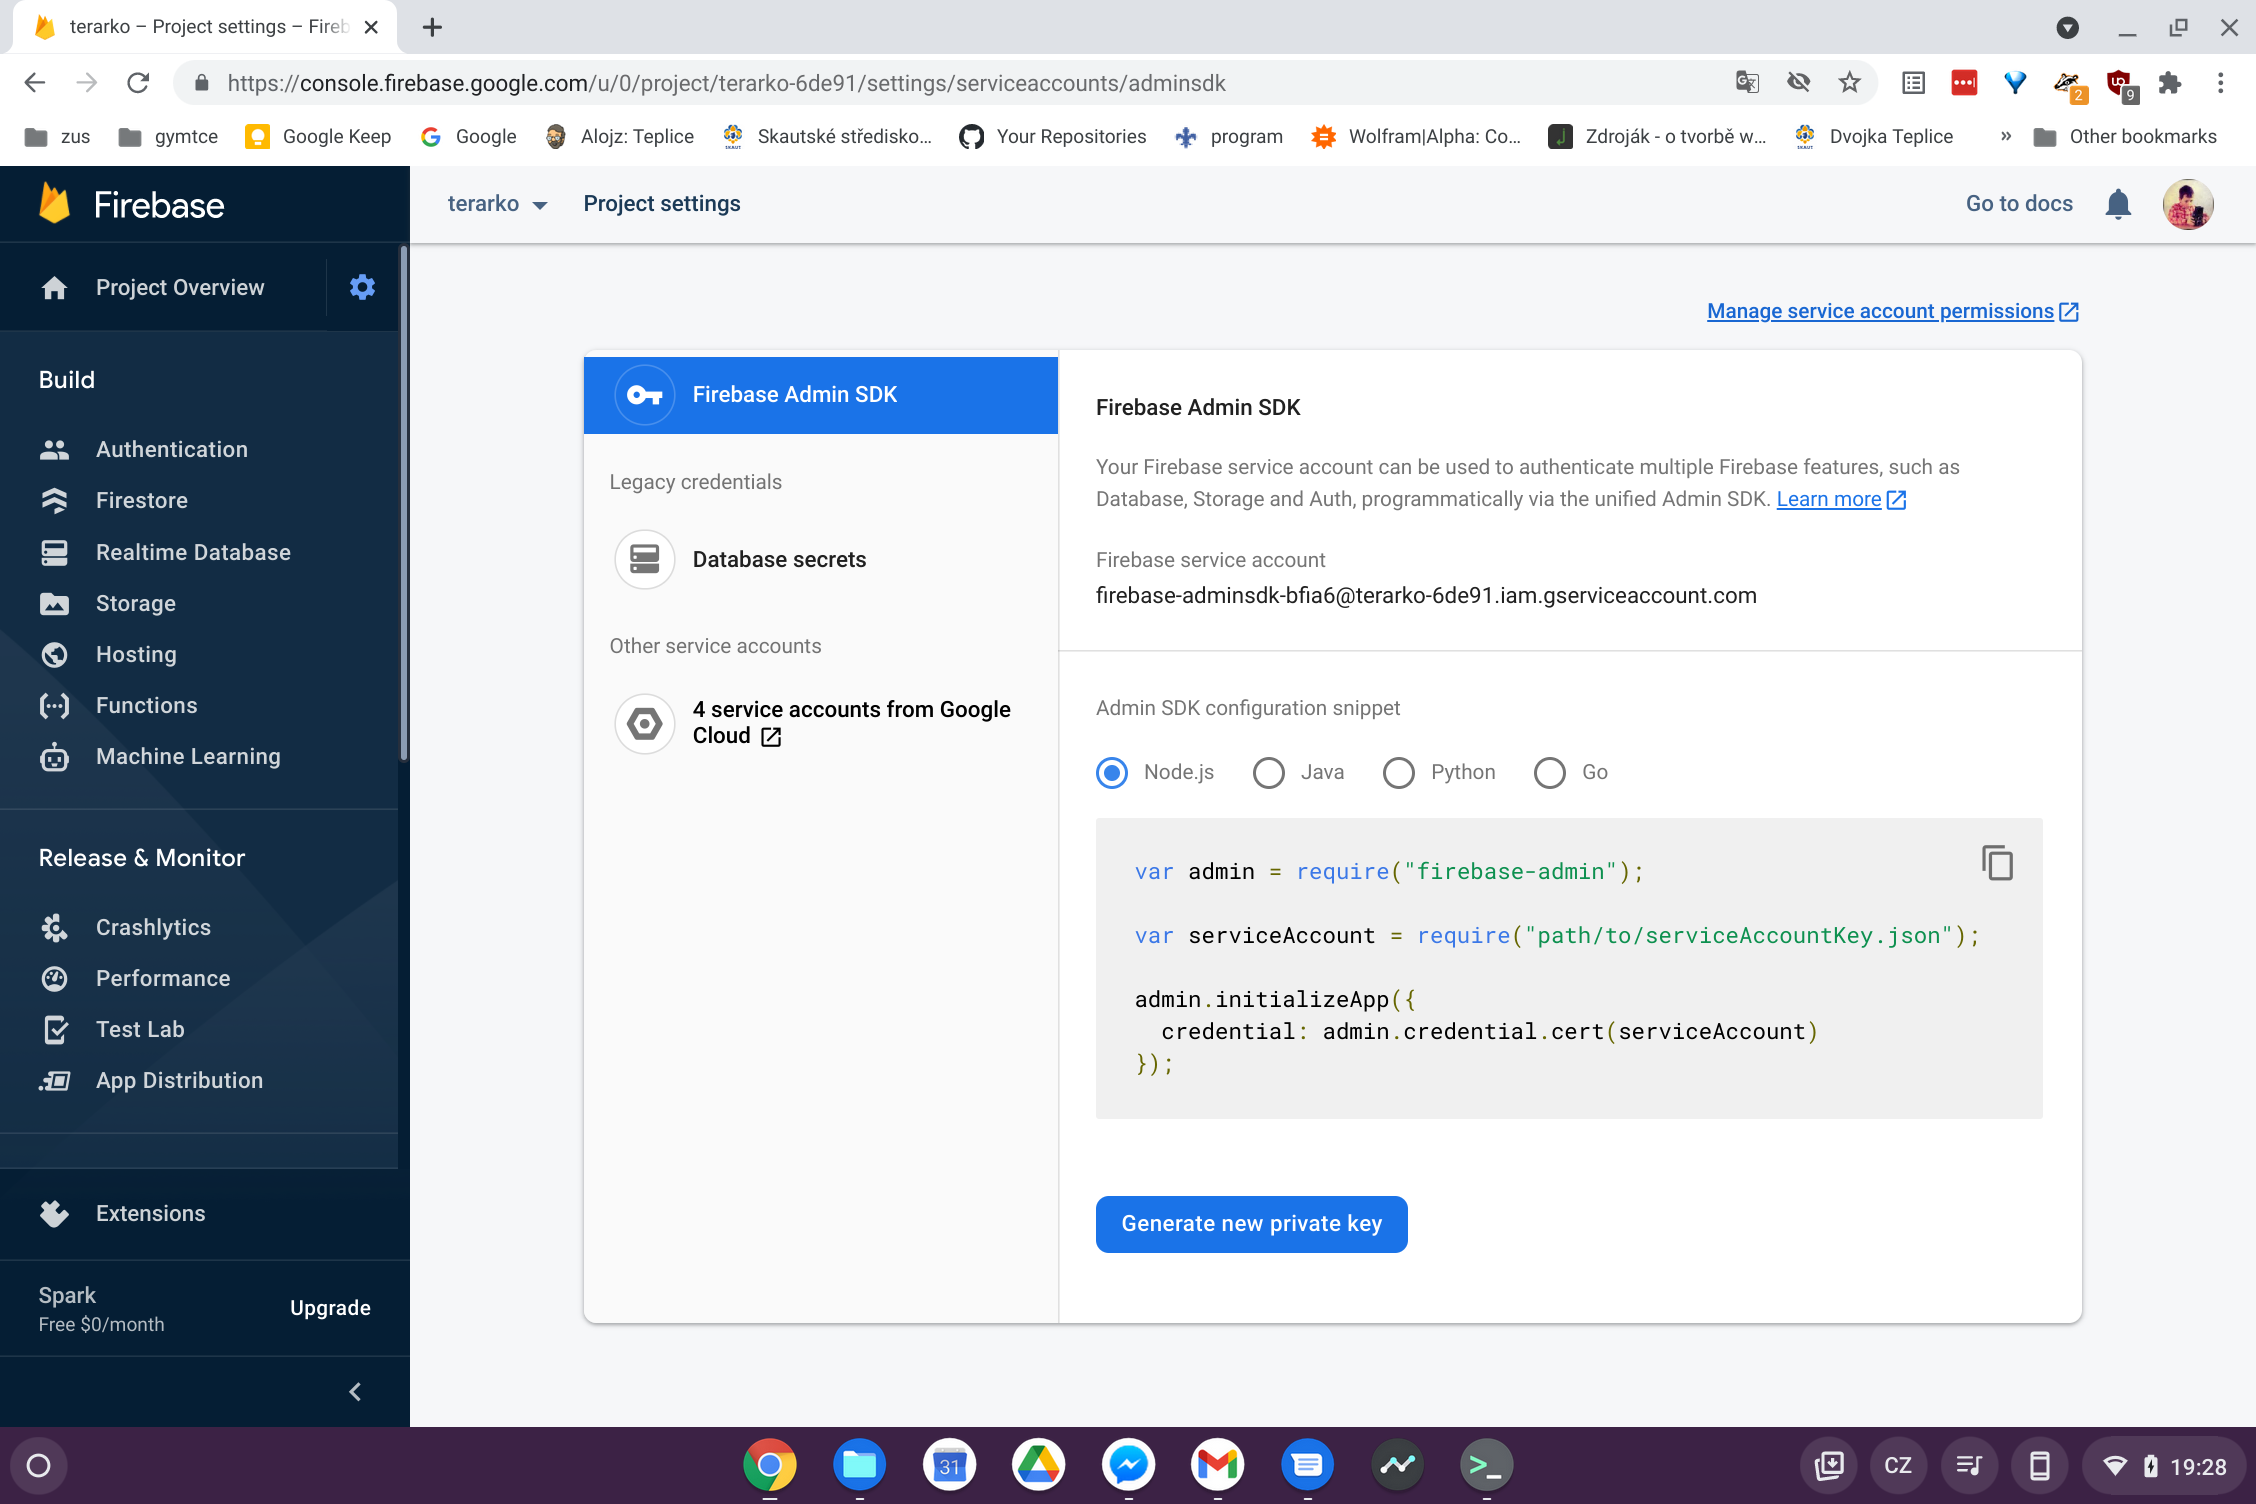
\includegraphics[width=0.8\textwidth]{key1.png}
    \caption{Vygenerování klíče, krok 1}
\end{figure}
% krok 2
\begin{figure}[H]
    \centering
    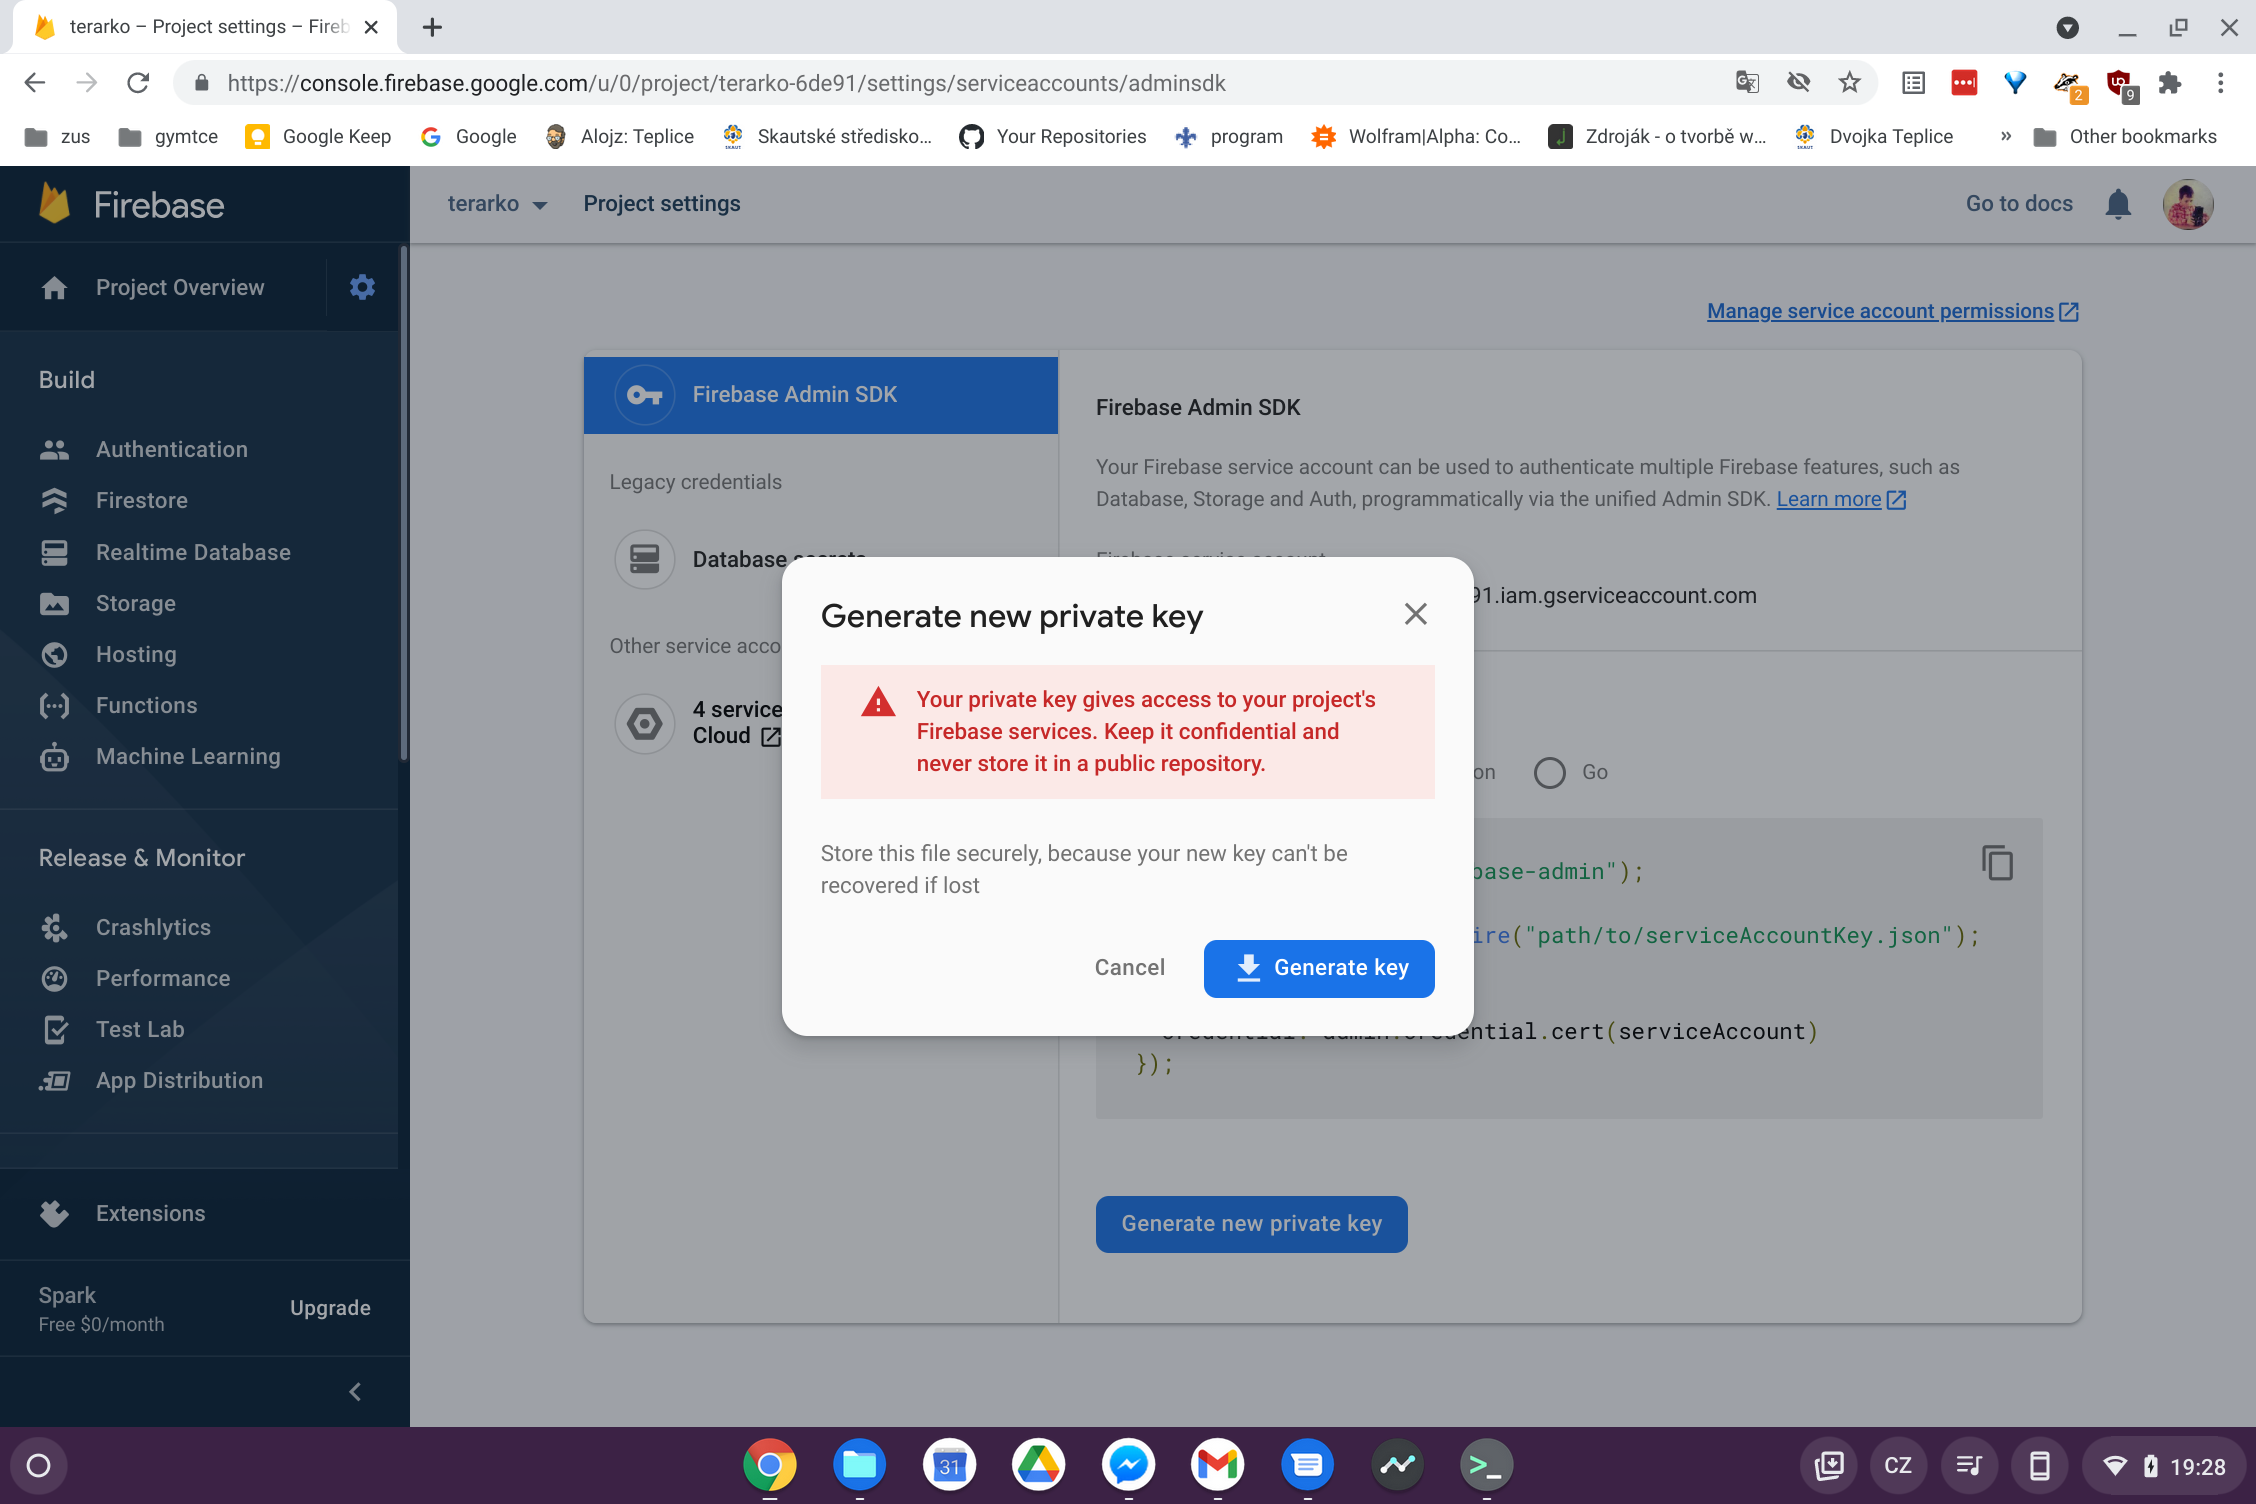
\includegraphics[width=0.8\textwidth]{key2.png}
    \caption{Vygenerování klíče, krok 2}
\end{figure}

\paragraph*{Organizace dat}
Pro každý senzor mám v databázi samostatnou kolekci, ve které je jedno měření představováno souborem, jenž obsahuje 
naměřená data a \gls{timestamp}. Název souboru nechávám generovat firestore, pro mě je nepodstatný.

\section{Zobrazení grafů}
% jak to bude vypadat
Pro potřeby zobrazení jsem se rozhodl vytvořit velmi jednoduchou \gls{spa}. Jediné co se na ní bude nacházet budou tři 
tlačítka pro přepínání mezi jednotlivými senzory a místo pro graf hodnot. Celá aplikace bude napsaná v javascriptu. 
Nejsem v něm úplně zběhlý, takže je možné, že některé konstrukce budou neoptimální, nebo přinejmenším podivné, avšak 
nemělo by to mít vliv na funkčnost. Koncept celé aplikace vypadá takto.

\begin{figure}[H]
  \centering
  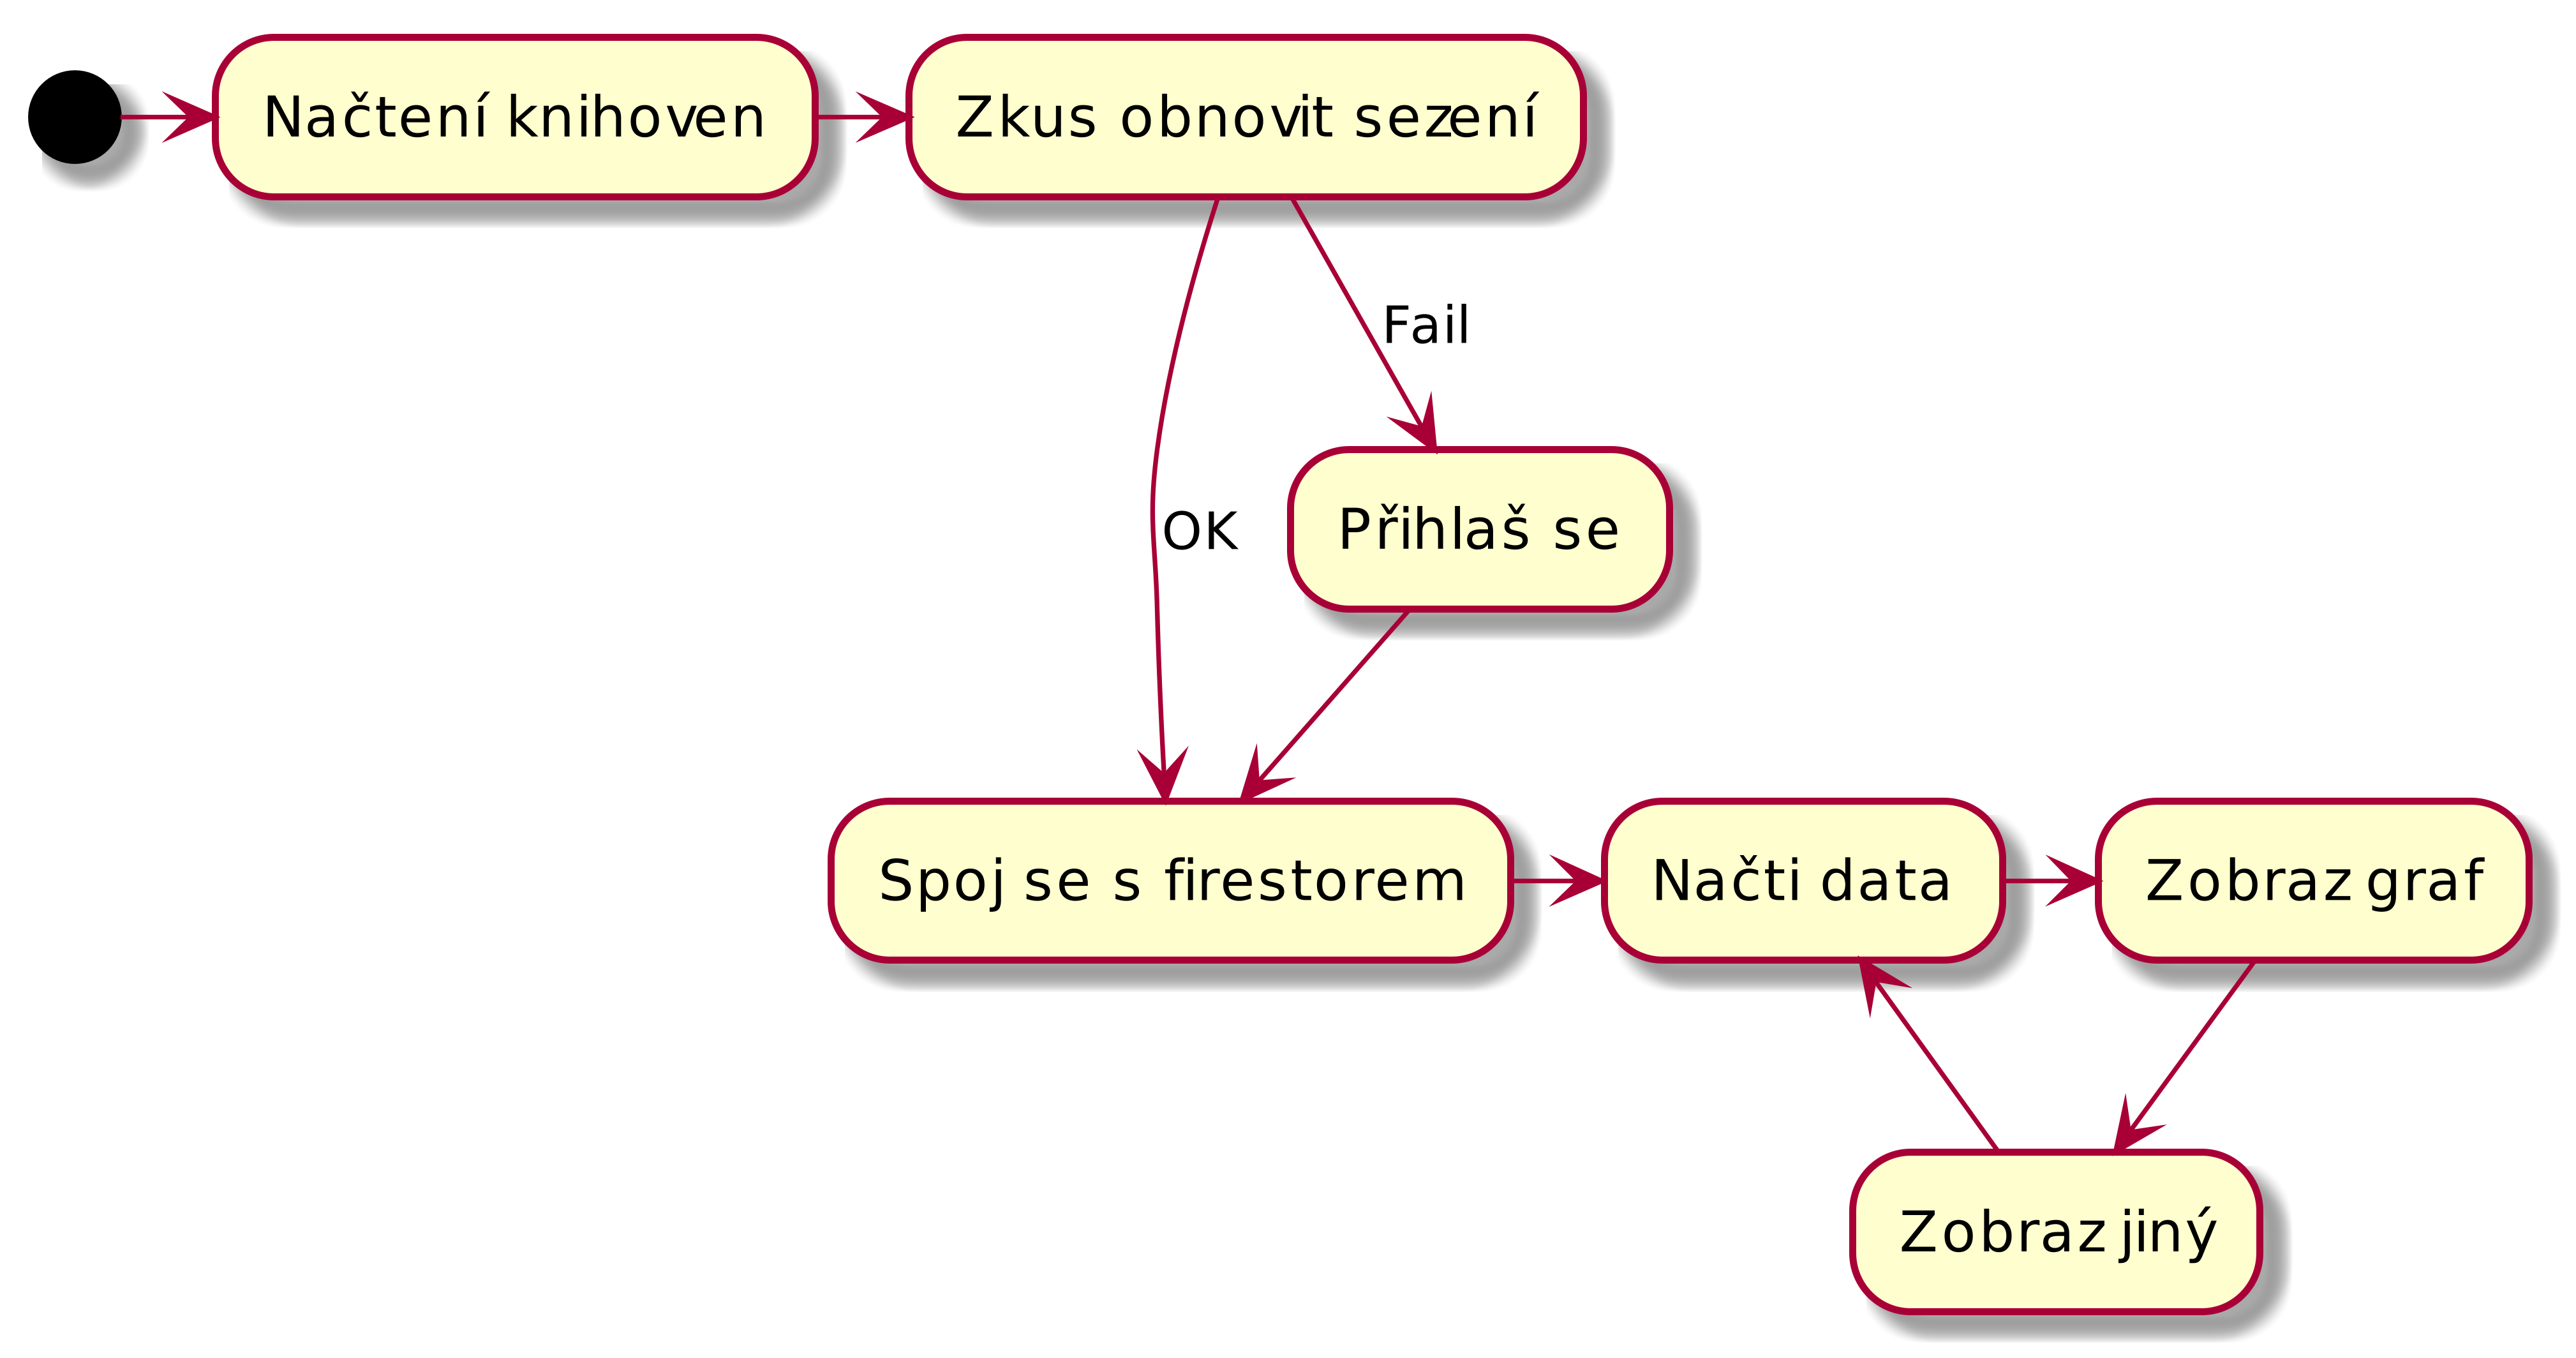
\includegraphics[width=\textwidth]{grafy.png}
  \caption{Průběh programu}
\end{figure}

Na začátku webové stránky, která tvoří kostru celého programu, načtu \gls{firebase} \glslink{knihovna}{knihovny}, 
vzhledem k tomu, že používám \gls{firebase} hosting, je tato část velmi jednoduchá, neb nemusím řešit autorizace\ldots 
Poté načtu \glslink{knihovna}{knihovnu} \gls{plotly}, kterou používám pro vykreslování grafů. Následně vytvořím 
přepínací tlačítka a plochu pro graf. Nakonec zavolám funkci co mi vykreslí graf hodnot v teráriu.

Do \gls{firebase} se přihlásím za použití \gls{oauth} u Googlu a to z jediného důvodu. Při nastavování Firestoru jsem 
nastavil pravidla tak, že bez přihlášení nikoho k datům nepustí. Takže jsem potřeboval nějak ověřit uživatele. Druhý 
problém byl, jak přesvědčit databázi, aby mi umožnila přístup k datům. Tady jsem použil místo řešení problémů 
s účty\ldots takový špinavý trik. Po přihlášení mi Google přidělil identifikátor, kterým se prokazuji vůči aplikaci, 
když jsem do pravidel přidal podmínku, že tento identifikátor může číst data, vše fungovalo. Není to řešení pro více 
uživatelů, ale dostačuje.

Následné vykreslení grafů už je v podstatě jen otázka, jak převést data z \gls{firebase} do pole. Začnu tím, že vyberu 
správnou kolekci, dle použitého senzoru, tu si seřadím podle \glslink{timestamp}{timestampu} a z ní vezmu posledních 192 
hodnot, což odpovídá cca posledním 48 hodinám. Následně pouze proiteruji přes všechna data a přidám je do pole hodnot, 
jediná výjimka je u času, který před tím převedu na čitelný tvar a do aktuálního časového pásma. Pak už data pouze 
vykreslím. Když mám v jednom grafu více datových polí, vykresluji je nad sebe se stejnou časovou osou, abych mohl 
porovnávat odpovídající hodnoty. Výsledek pak vypadá nějak takto.

% obrázky grafů
% BME280
\begin{figure}[H]
    \centering
    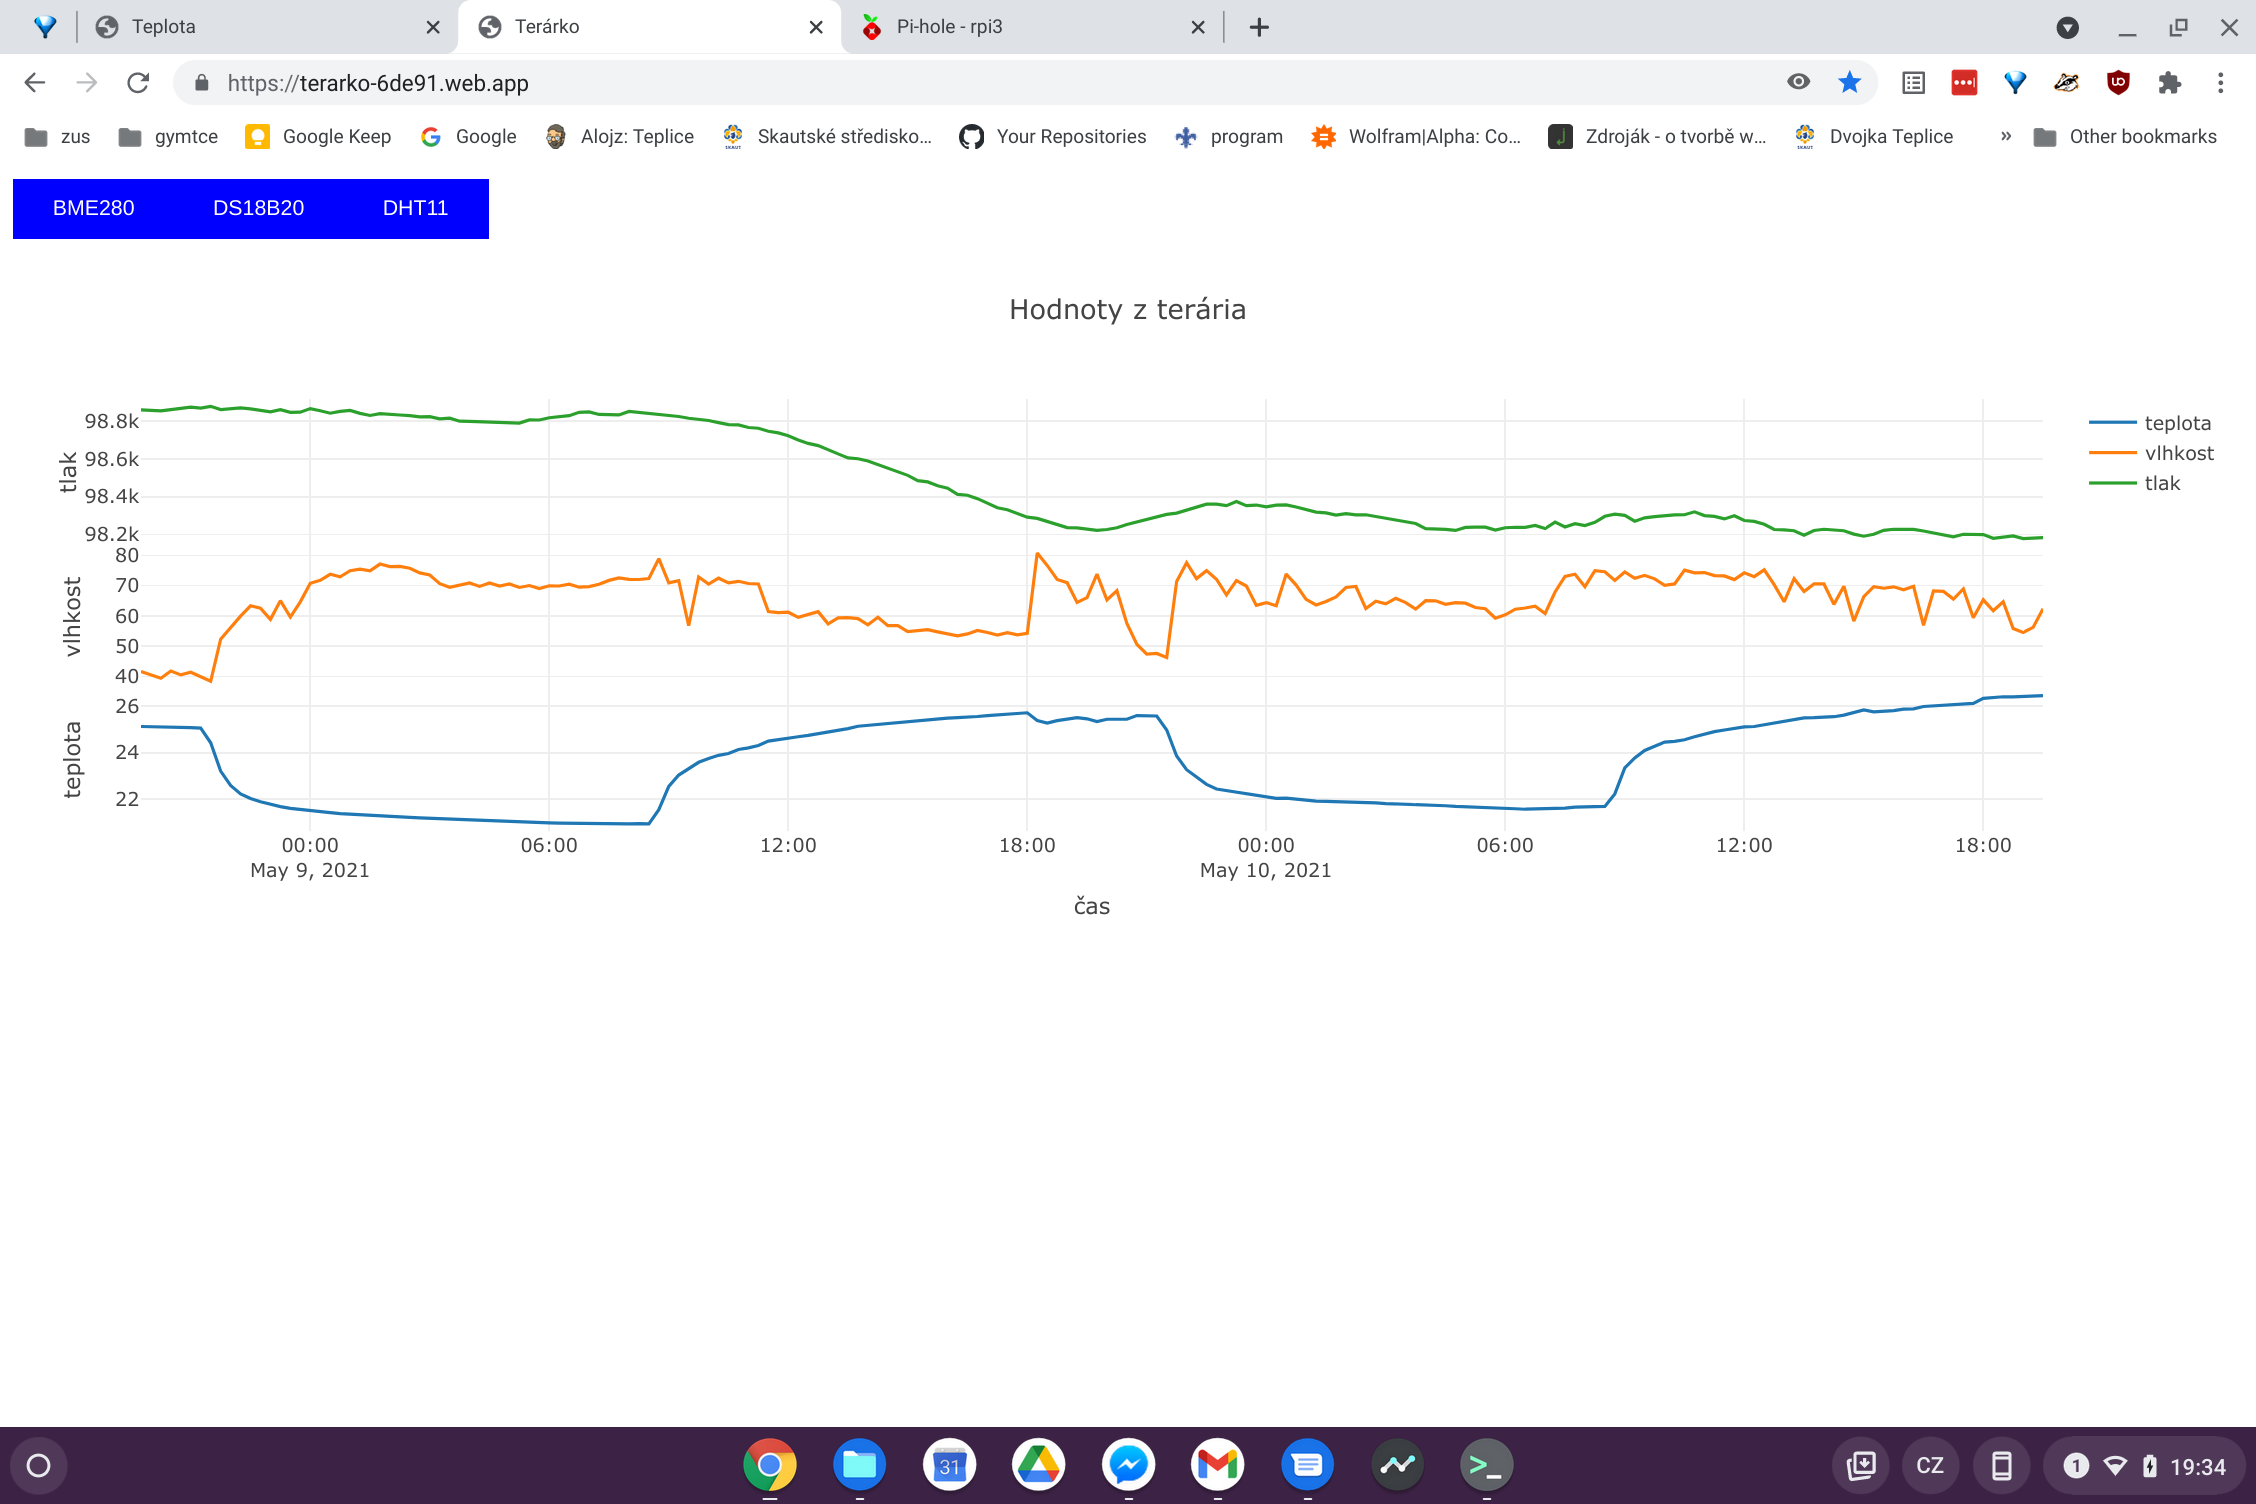
\includegraphics[width=0.8\textwidth]{BME280-graf.png}
    \caption{Data z terária}
\end{figure}
% DS18B20
\begin{figure}[H]
    \centering
    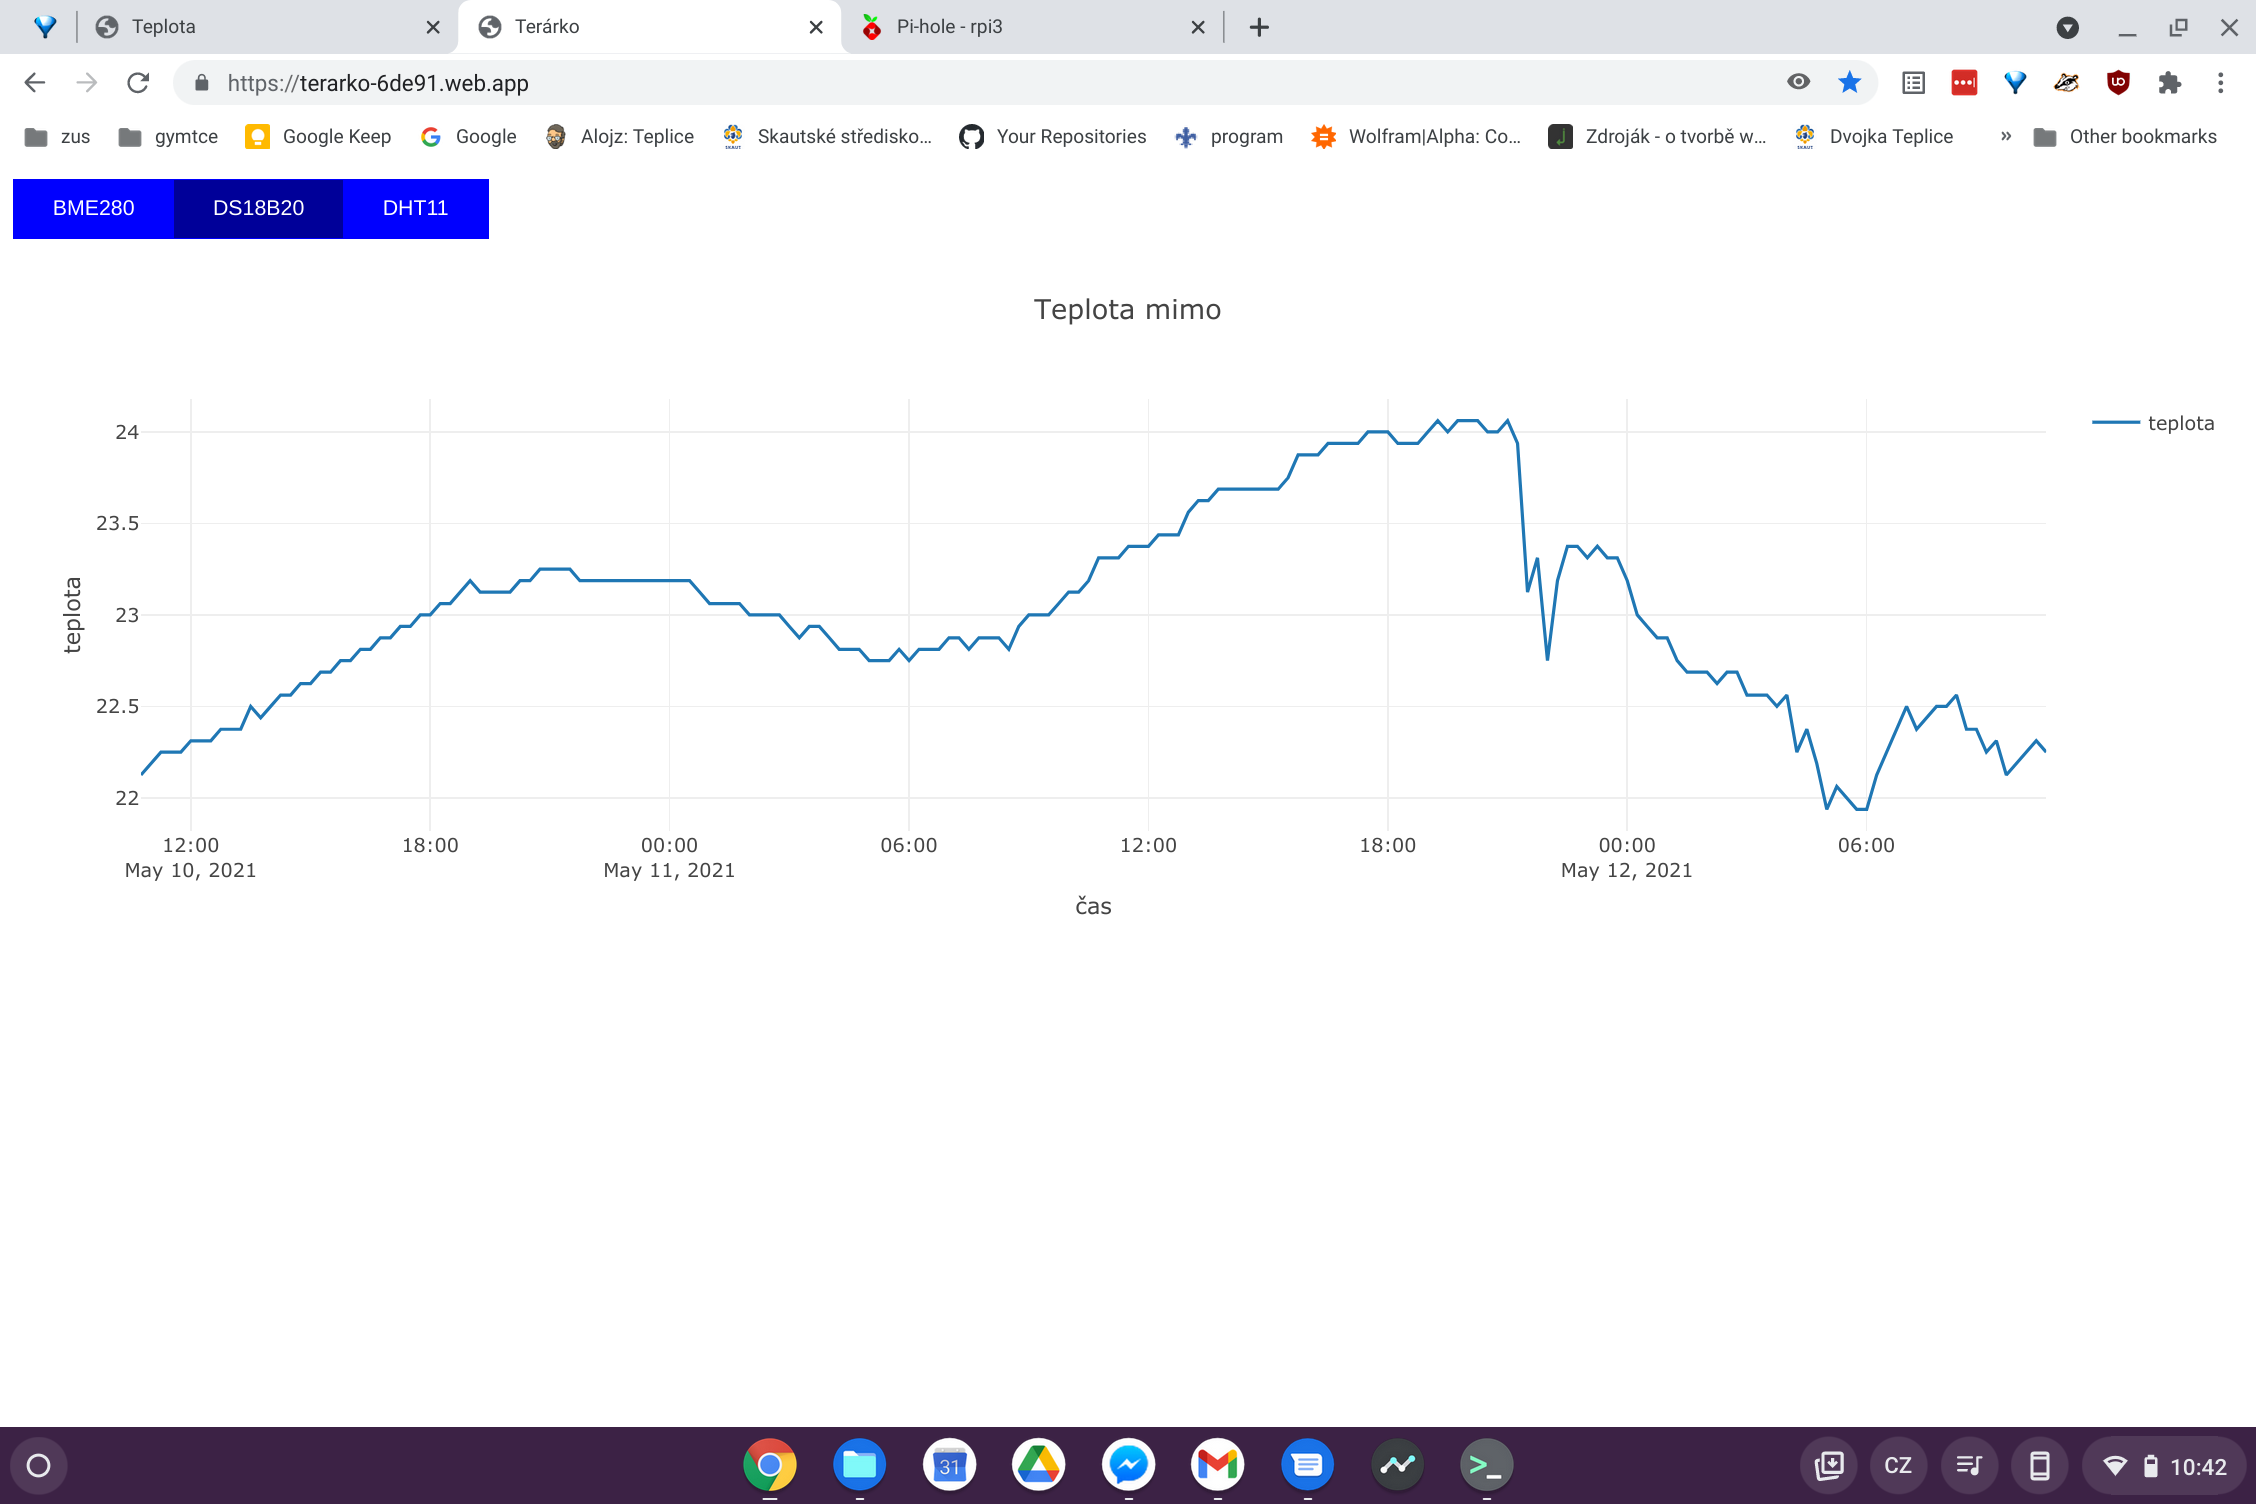
\includegraphics[width=0.8\textwidth]{DS18B20-graf.png}
    \caption{Teplota mimo terárium}
\end{figure}
% DHT11
\begin{figure}[H]
    \centering
    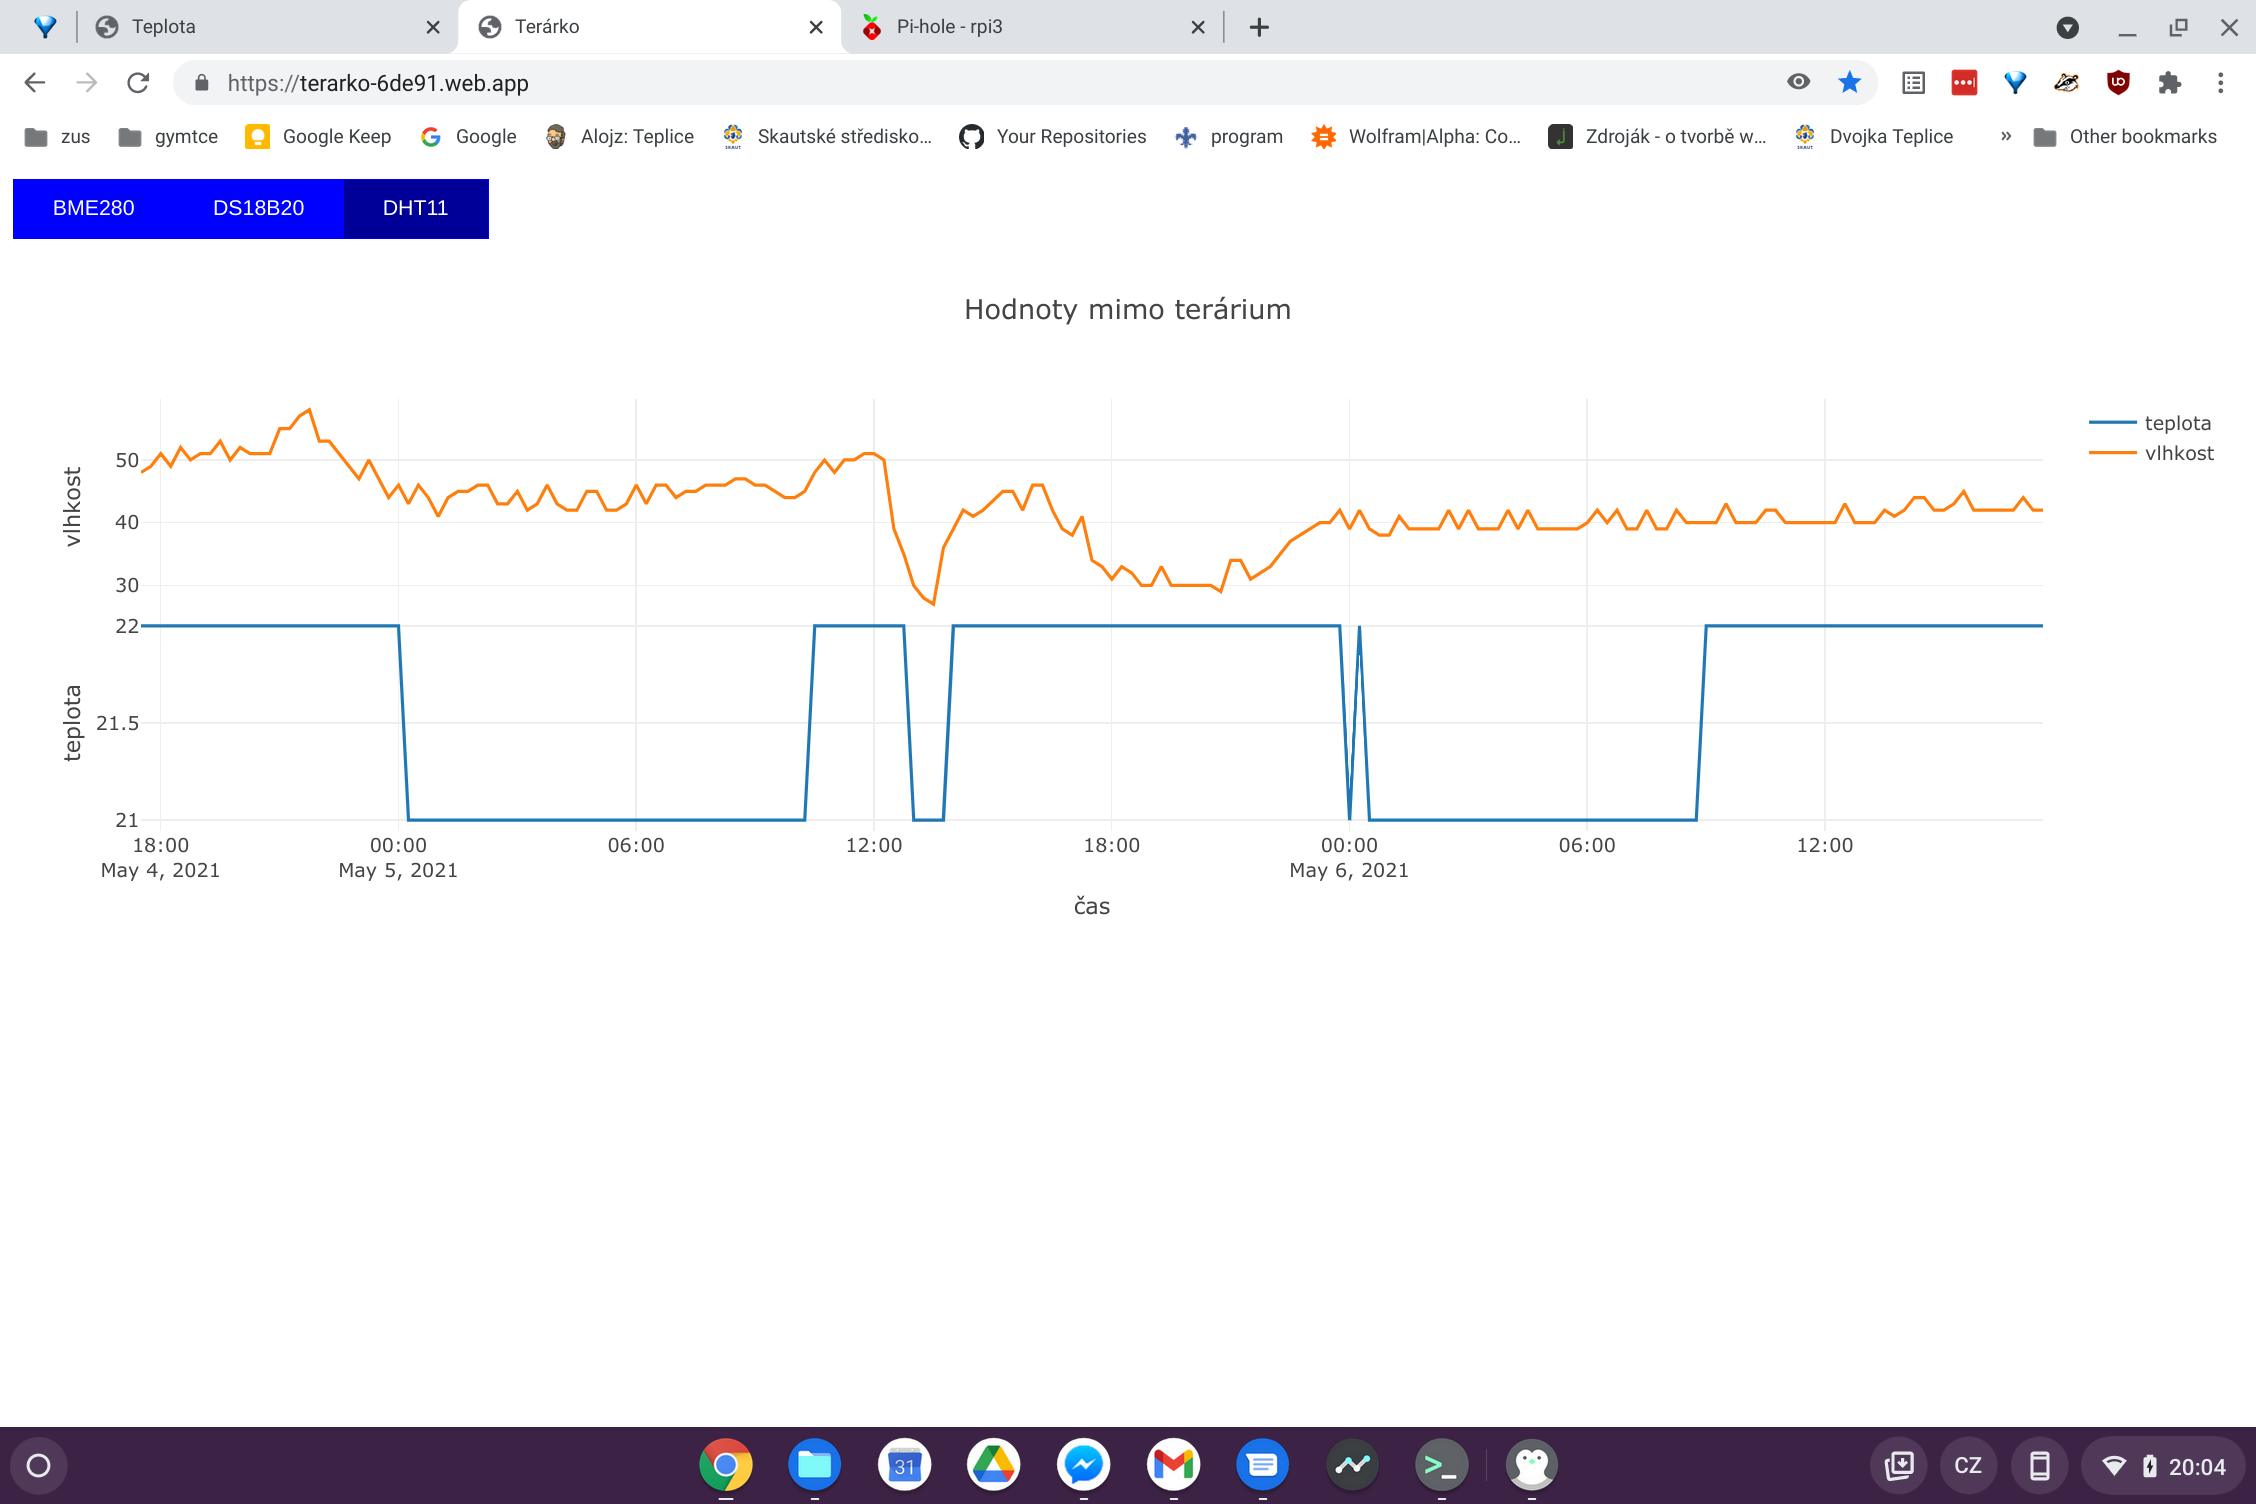
\includegraphics[width=0.8\textwidth]{DHT11-graf.png}
    \caption{Teplota a vlhkost mimo terárium}
\end{figure}

